\documentclass[]{article}
\usepackage{lmodern}
\usepackage{amssymb,amsmath}
\usepackage{ifxetex,ifluatex}
\usepackage{fixltx2e} % provides \textsubscript
\ifnum 0\ifxetex 1\fi\ifluatex 1\fi=0 % if pdftex
  \usepackage[T1]{fontenc}
  \usepackage[utf8]{inputenc}
\else % if luatex or xelatex
  \ifxetex
    \usepackage{mathspec}
  \else
    \usepackage{fontspec}
  \fi
  \defaultfontfeatures{Ligatures=TeX,Scale=MatchLowercase}
\fi
% use upquote if available, for straight quotes in verbatim environments
\IfFileExists{upquote.sty}{\usepackage{upquote}}{}
% use microtype if available
\IfFileExists{microtype.sty}{%
\usepackage{microtype}
\UseMicrotypeSet[protrusion]{basicmath} % disable protrusion for tt fonts
}{}
\usepackage[margin=1in]{geometry}
\usepackage{hyperref}
\hypersetup{unicode=true,
            pdftitle={Reinführung in RStudio},
            pdfauthor={Walter Gruber},
            pdfborder={0 0 0},
            breaklinks=true}
\urlstyle{same}  % don't use monospace font for urls
\usepackage{color}
\usepackage{fancyvrb}
\newcommand{\VerbBar}{|}
\newcommand{\VERB}{\Verb[commandchars=\\\{\}]}
\DefineVerbatimEnvironment{Highlighting}{Verbatim}{commandchars=\\\{\}}
% Add ',fontsize=\small' for more characters per line
\usepackage{framed}
\definecolor{shadecolor}{RGB}{248,248,248}
\newenvironment{Shaded}{\begin{snugshade}}{\end{snugshade}}
\newcommand{\KeywordTok}[1]{\textcolor[rgb]{0.13,0.29,0.53}{\textbf{#1}}}
\newcommand{\DataTypeTok}[1]{\textcolor[rgb]{0.13,0.29,0.53}{#1}}
\newcommand{\DecValTok}[1]{\textcolor[rgb]{0.00,0.00,0.81}{#1}}
\newcommand{\BaseNTok}[1]{\textcolor[rgb]{0.00,0.00,0.81}{#1}}
\newcommand{\FloatTok}[1]{\textcolor[rgb]{0.00,0.00,0.81}{#1}}
\newcommand{\ConstantTok}[1]{\textcolor[rgb]{0.00,0.00,0.00}{#1}}
\newcommand{\CharTok}[1]{\textcolor[rgb]{0.31,0.60,0.02}{#1}}
\newcommand{\SpecialCharTok}[1]{\textcolor[rgb]{0.00,0.00,0.00}{#1}}
\newcommand{\StringTok}[1]{\textcolor[rgb]{0.31,0.60,0.02}{#1}}
\newcommand{\VerbatimStringTok}[1]{\textcolor[rgb]{0.31,0.60,0.02}{#1}}
\newcommand{\SpecialStringTok}[1]{\textcolor[rgb]{0.31,0.60,0.02}{#1}}
\newcommand{\ImportTok}[1]{#1}
\newcommand{\CommentTok}[1]{\textcolor[rgb]{0.56,0.35,0.01}{\textit{#1}}}
\newcommand{\DocumentationTok}[1]{\textcolor[rgb]{0.56,0.35,0.01}{\textbf{\textit{#1}}}}
\newcommand{\AnnotationTok}[1]{\textcolor[rgb]{0.56,0.35,0.01}{\textbf{\textit{#1}}}}
\newcommand{\CommentVarTok}[1]{\textcolor[rgb]{0.56,0.35,0.01}{\textbf{\textit{#1}}}}
\newcommand{\OtherTok}[1]{\textcolor[rgb]{0.56,0.35,0.01}{#1}}
\newcommand{\FunctionTok}[1]{\textcolor[rgb]{0.00,0.00,0.00}{#1}}
\newcommand{\VariableTok}[1]{\textcolor[rgb]{0.00,0.00,0.00}{#1}}
\newcommand{\ControlFlowTok}[1]{\textcolor[rgb]{0.13,0.29,0.53}{\textbf{#1}}}
\newcommand{\OperatorTok}[1]{\textcolor[rgb]{0.81,0.36,0.00}{\textbf{#1}}}
\newcommand{\BuiltInTok}[1]{#1}
\newcommand{\ExtensionTok}[1]{#1}
\newcommand{\PreprocessorTok}[1]{\textcolor[rgb]{0.56,0.35,0.01}{\textit{#1}}}
\newcommand{\AttributeTok}[1]{\textcolor[rgb]{0.77,0.63,0.00}{#1}}
\newcommand{\RegionMarkerTok}[1]{#1}
\newcommand{\InformationTok}[1]{\textcolor[rgb]{0.56,0.35,0.01}{\textbf{\textit{#1}}}}
\newcommand{\WarningTok}[1]{\textcolor[rgb]{0.56,0.35,0.01}{\textbf{\textit{#1}}}}
\newcommand{\AlertTok}[1]{\textcolor[rgb]{0.94,0.16,0.16}{#1}}
\newcommand{\ErrorTok}[1]{\textcolor[rgb]{0.64,0.00,0.00}{\textbf{#1}}}
\newcommand{\NormalTok}[1]{#1}
\usepackage{longtable,booktabs}
\usepackage{graphicx,grffile}
\makeatletter
\def\maxwidth{\ifdim\Gin@nat@width>\linewidth\linewidth\else\Gin@nat@width\fi}
\def\maxheight{\ifdim\Gin@nat@height>\textheight\textheight\else\Gin@nat@height\fi}
\makeatother
% Scale images if necessary, so that they will not overflow the page
% margins by default, and it is still possible to overwrite the defaults
% using explicit options in \includegraphics[width, height, ...]{}
\setkeys{Gin}{width=\maxwidth,height=\maxheight,keepaspectratio}
\IfFileExists{parskip.sty}{%
\usepackage{parskip}
}{% else
\setlength{\parindent}{0pt}
\setlength{\parskip}{6pt plus 2pt minus 1pt}
}
\setlength{\emergencystretch}{3em}  % prevent overfull lines
\providecommand{\tightlist}{%
  \setlength{\itemsep}{0pt}\setlength{\parskip}{0pt}}
\setcounter{secnumdepth}{5}
% Redefines (sub)paragraphs to behave more like sections
\ifx\paragraph\undefined\else
\let\oldparagraph\paragraph
\renewcommand{\paragraph}[1]{\oldparagraph{#1}\mbox{}}
\fi
\ifx\subparagraph\undefined\else
\let\oldsubparagraph\subparagraph
\renewcommand{\subparagraph}[1]{\oldsubparagraph{#1}\mbox{}}
\fi

%%% Use protect on footnotes to avoid problems with footnotes in titles
\let\rmarkdownfootnote\footnote%
\def\footnote{\protect\rmarkdownfootnote}

%%% Change title format to be more compact
\usepackage{titling}

% Create subtitle command for use in maketitle
\newcommand{\subtitle}[1]{
  \posttitle{
    \begin{center}\large#1\end{center}
    }
}

\setlength{\droptitle}{-2em}

  \title{Reinführung in RStudio}
    \pretitle{\vspace{\droptitle}\centering\huge}
  \posttitle{\par}
    \author{Walter Gruber}
    \preauthor{\centering\large\emph}
  \postauthor{\par}
      \predate{\centering\large\emph}
  \postdate{\par}
    \date{2019-01-20}


\begin{document}
\maketitle

{
\setcounter{tocdepth}{2}
\tableofcontents
}
\section*{Vorwort}\label{vorwort}
\addcontentsline{toc}{section}{Vorwort}

Dieser Kurs richtet sich vor allem an jene Personen, die weder
Erfahrungen in der Programmierung im Allgemeinen, noch im Umgang mit R
im Speziellen haben. Programme zu schreiben ist nicht allzu schwer. Man
muss sich ein paar Regeln der verwendeten Programmiersprache aneignen
und schon kann es losgehen.

Gute Programme zu schreiben ist schon etwas schwieriger, aber auch das
ist mit etwas Aufwand durchaus machbar. Häufig wird am Beginn einer
Karriere als Programmierer der Fehler gemacht, sich zu sehr auf Details
zu konzentrieren und dabei den Überblick des eigentlichen Ziels eines
Programmes zu verlieren. Während der Programmierung sollte man sich
stets darüber im Klaren sein, dass ein Computerprogramm immer genau das
macht, was man ihm sagt und nichts macht, was man ihm nicht sagt.

Was uns oft klar und logisch erscheint, bleibt für ein Computerprogramm
so lange undurchführbar, bis man es durch detaillierte Schritt für
Schritt Instruktionen mit unserer Logik und Idee vertraut gemacht hat.
Wenn das gelingt, wird es ein treuer Partner sein und mit einer
unbestechlichen Präzision diese Logik hunderte, oder millionenmal
abarbeiten, ohne einen einzigen Fehler dabei zu begehen.

Für Einsteiger ist es oft schwierig zu beurteilen, in welcher
Reihenfolge und in welchem Detail Instruktionen für den Computer gegeben
werden müssen. Daher ist es primäres Ziel dieser LV, die grundlegenden
Elemente der Programmiersprache R kennen zulernen und diese richtig
anzuwenden. Dabei werden wir auch Hilfsmittel kennen lernen, die den
Einstieg in R wesentlich erleichtern können.

\section{Aufbau des Kurses}\label{aufbau-des-kurses}

\begin{figure}
\centering

\includegraphics[width=0.50000\textwidth]{Images/Cover.png}
\caption{}
\end{figure}

Im Lauf des Kurses werden wir abwechselnd zwei unterschiedliche Ansätze
des Lernens verwenden. Ich habe diese Ansätze \emph{Top-Down} und
\emph{Bottom-Up} genannt und werde die Idee dahinter noch im Detail
erklären. Der Einstieg in R wird wesentlich durch die Verwendung von
\emph{RStudio} erleichtert. Wir werden im Folgenden die Eigenschaften
und den Umgang mit diesem Programm im Detail besprechen.

Unabhängig von der Vorgehensweise werden wir jeweils zu den behandelten
Themen direkt Übungen in R durchführen. Diese Übungen sind zum Großteil
in den vorliegenden Unterlagen beschrieben und der entsprechende R-Code
kann direkt aus diesen Unterlagen ins \emph{RStudio} übernommen und
ausgeführt werden.

Des Weiteren sind zwischen den Kursterminen Hausübungen zu bearbeiten.
Den genauen Ablauf werde ich während der Lehrveranstaltung bekannt
geben. Zur Beurteilung eurer Leistungen in der LV sind interaktive
Online-Fragen zu bearbeiten. Auch hierzu werde ich Details während der
LV bekannt geben.

\subsection*{Ziele}\label{ziele}
\addcontentsline{toc}{subsection}{Ziele}

\begin{itemize}
\tightlist
\item
  Aufbau von R-Studio.
\item
  wo und wie findet man nützliche Infos zu R und RStudio.
\item
  Definition von Daten und Objekten in R
\item
  grundlegende Logik von Befehlen und Funktionen in R.
\item
  Daten einlesen und bearbeiten.
\item
  einfache deskriptive Statistiken anfordern.
\item
  einfache Graphiken erstellen und bearbeiten.
\item
  einige nützliche (statistische) Funktionen kennen.
\end{itemize}

\subsection*{Allgemeines}\label{allgemeines}
\addcontentsline{toc}{subsection}{Allgemeines}

Nachfolgend ein kurzer Überblick über die Entstehungsgeschichte von R.

\subsubsection*{\texorpdfstring{Entstehungsgeschichte von R\footnote{\href{https://de.wikipedia.org/wiki/R_(Programmiersprache)\#Urspr\%C3\%BCnge_(1992)}{Geschichte
  von R - Wikipedia}}}{Entstehungsgeschichte von R}}\label{entstehungsgeschichte-von-r1}
\addcontentsline{toc}{subsubsection}{Entstehungsgeschichte von R}

\begin{figure}
\centering
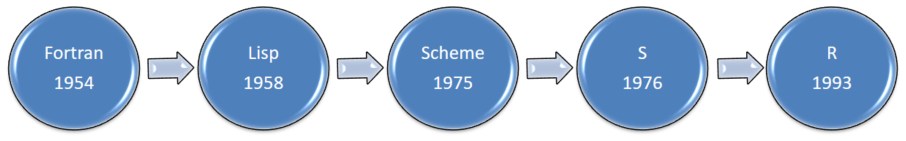
\includegraphics[width=0.50000\textwidth]{Images/RHistorie.png}
\caption{\textbf{Abbildung 1}: von F zu R}
\end{figure}

\begin{itemize}
\tightlist
\item
  Entwickelt 1992, orientiert sich R eng an Sprache S. Weitere
  Inspirationsquelle war die Programmiersprache Scheme. \textbf{1993
  wurde die Software erstmals öffentlich vorgestellt} und seit Juni 1995
  steht R unter der
  \href{https://de.wikipedia.org/wiki/GNU_General_Public_License}{GNU
  General Public License}.
\item
  Bis 1996 oder 1997 gab es zwischen 50 und 100 Leute in einer
  Mailingliste, die dabei halfen die Sprache gemeinsam zu verbessern. Im
  Jahr 1997 wurde das R Development Core Team gebildet (heute R Core
  Team), das sich um die Weiterentwicklung von R kümmert und den
  Quellcode verändern kann.
\item
  Das Comprehensive R Archive Network (CRAN) als Plattform für Pakete
  startete am 23. April 1997 um Anwendern die Möglichkeit zu geben
  selbst geschriebene Funktionen leichter mit Anderen zu teilen.
\item
  Seit April 2001 gibt es R für macOS. Im September 2002 gründeten die
  Mitglieder des R Development Core Teams den gemeinnützigen Verein The
  R Foundation for Statistical Computing in Wien, welcher sich um die
  Außendarstellung kümmert.
\item
  Die R-Version 2.0 wurde am 4. Oktober 2004 veröffentlicht. Seitdem
  nutzt R Lazy Loading, um Daten bei geringer Beanspruchung des
  Arbeitsspeichers schnell laden zu können.
\item
  Ab Version 2.1 (18. April 2005) unterstützt R unterschiedliche
  Sprachversionen (Internationalisierung) und Zeichenkodierungen,
  insbesondere UTF-8.
\item
  Mit die Einführung von Version 2.11 im April 2010, die R auf
  64-Bit-Systemen nutzbar macht und bis zu acht Terabyte Arbeitsspeicher
  adressieren kann gelang der Einstieg in Big-Data-Processing.
\item
  Im Oktober 2011 (Version 2.14) wurde die parallele Ausführung von
  Funktionen eingeführt.
\item
  Neben all diesen technischen Entwicklungen wurden unzählige Pakete für
  alle erdenklichen Anwendungsbereiche durch die Community entwickelt.
\item
  Derzeit (Stand November 2018) gibt es 13.346 packages (mit dem Befehl
  \emph{available.packages()}) kann man das jederzeit abfragen) allein
  auf CRAN! Dabei sind die Packages anderer Repositories (z.B.
  \emph{Bioconductor}\footnote{\href{https://www.bioconductor.org/}{Bioconductor
    - Software for Bioinformatics}} mit 1.649 packages) noch nicht
  berücksichtigt!
\end{itemize}

\subsubsection*{\texorpdfstring{\textbf{Warum} sollte man \textbf{R}
verwenden?}{Warum sollte man R verwenden?}}\label{warum-sollte-man-r-verwenden}
\addcontentsline{toc}{subsubsection}{\textbf{Warum} sollte man
\textbf{R} verwenden?}

R ist eine Programmiersprache, die besonders zur Analyse und
Visualisierung von Daten genutzt wird. Sehr viele Neuentwicklungen in
der Statistik passieren in R. Auch ohne Vorkenntnisse in einer
Programmiersprache findet man sich in R schnell zurecht.

Mit Hilfe von RStudio, den unzähligen Tutorials und Hilfeseiten gelingt
es schon nach sehr kurzer Zeit die ersten hilfreichen Programme zu
schreiben. Alle diese Tools sind
\href{https://de.wikipedia.org/wiki/Open_Source}{open source}, d.h.
transparent, eigenständig veränderbar und vor allem kostenlos. Stellt
man die Vor- und Nachteile der Nutzung von R gegenüber, lässt sich die
Entscheidung Arbeit in R hineinzustecken relativ leicht rechtfertigen:

\begin{itemize}
\tightlist
\item
  Vorteile

  \begin{itemize}
  \tightlist
  \item
    Neben gängigen Programmen zur statistischen Auswertung, wie
    beispielsweise ``SPSS'' bietet R den Vorteil, dass es auf der ganzen
    Welt kostenlos zur Verfügung steht.
  \item
    R kann die meisten gängigen Formate importieren und bietet ein
    quelloffenes Format für erstellte Datensätze.
  \item
    Darüber hinaus stellt R mächtigere und mehr Auswertungsverfahren zur
    Verfügung als viele andere Programme.
  \item
    R ist eine Programmierumgebung. Funktionen können bequem den eigenen
    Bedürfnissen angepasst werden. Komplexe Probleme lassen sich auch
    dann lösen, wenn die Entwickler diese (noch) nicht implementiert
    haben.
  \item
    R wird von der Scientific Community kontinuierlich weiterentwickelt.
    Neue statistische Verfahren werden in der Regel auch in R
    integriert. Ein standardisiertes Pakete-System erleichtert die
    Nachinstallation ebenso wie die Veröffentlichung eigener Pakete.
  \item
    R erstellt professionelle Graphiken in einer Vielzahl an Formaten.
  \item
    R erleichtert durch z.T. selbstdokumentierende Codes die
    Reproduzierbarkeit von Studien.
  \item
    R bietet eine Vielzahl an Online-Tutorials, Blogs und sonstige
    Hilfestellungen.
  \end{itemize}
\item
  Nachteile

  \begin{itemize}
  \tightlist
  \item
    Für den Anfänger ist die Funktionsweise und Bedienung von R
    zweifellos gewöhnungsbedürftig.
  \item
    die Formatierung von Ergebnisse in R (Tabellen, Graphiken, etc.)
    muss häufig durch zusätzliche Programmschritte vom Benutzer
    durchgeführt werden.
  \item
    R ist prinzipiell Code-basiert. Benutzerfreundliche
    Interaktionsfenster zur Parametrisierung von Analysen müssen durch
    den Programmierer mit Hilfe entsprechender Programmpakete (z.B.
    Shiny, Java, etc.) selbst erstellt werden.
  \end{itemize}
\end{itemize}

\subsubsection*{\texorpdfstring{\textbf{Wann} sollte man \textbf{R}
verwenden?}{Wann sollte man R verwenden?}}\label{wann-sollte-man-r-verwenden}
\addcontentsline{toc}{subsubsection}{\textbf{Wann} sollte man \textbf{R}
verwenden?}

Ein Hardco\emph{R}e'\emph{ler} würde diese Frage nicht verstehen und
sich wahrscheinlich kopfschüttelnd wieder der Programmierung widmen,
ohne den Fragesteller weiter zu beachten. Für alle anderen stellt sich
jedoch die Frage, ob und ab wann sich der Aufwand eine
Programmiersprache zu erlernen lohnt. Das kann eigentlich nur jeder für
sich selbst entscheiden. Gute Gründe könnten z.B. sein, wenn:

\begin{itemize}
\tightlist
\item
  keine finanziellen Mittel zur Anschaffung einer kostenpflichtigen
  Statistiksoftware vorhanden sind.
\item
  die zur Verfügung stehende Software ist nicht in der Lage, ein
  vorliegendes statistisches Problem zu lösen.
\item
  man in einem Team eine Auswertungsstrategie (sanity checks,
  Standardprozeduren, etc.) entwickeln möchte.
\item
  dynamisches Reporting im Ablauf eines Forschungsprozesses verwendet
  werden soll.
\end{itemize}

\subsubsection*{\texorpdfstring{\textbf{Wann} sollte man \textbf{R
nicht}
verwenden?}{Wann sollte man R nicht verwenden?}}\label{wann-sollte-man-r-nicht-verwenden}
\addcontentsline{toc}{subsubsection}{\textbf{Wann} sollte man \textbf{R
nicht} verwenden?}

Geht es einzig und allein darum, einen Datensatz explorativ und/oder mit
gängigen Analysemethoden zu bearbeiten, kann man auf bereits bestehende
und benutzerfreundliche Anwendungen zurückgreifen. Wir werden uns im
folgenden zwei durchaus brauchbare Programmpakete kurz ansehen.

Stehen Programme wie SPSS, SAS o.ä. zur Verfügung, sollte man sich vor
den Einstieg in R klar über die gesteckten Ziele sein und eine
Kosten-Nutzen-Rechnung anstellen. Sehr oft ist es viel einfacher, sich
in die Syntax des jeweiligen Programms einzuarbeiten, als alles in R zu
lösen. Es sei auch darauf hingewiesen, dass (zumindest)
\href{https://www.ibm.com/support/knowledgecenter/de/SSLVMB_25.0.0/statistics_r_tutorial_project_ddita/spss/tutorials/rtut_intro.html}{SPSS
bereits eine Schnittstelle mit R} anbietet. Details dazu sind in den
entsprechenden Manuals nachzulesen.

Weitere wichtige Überlegungen bezüglich der Umstellung/Einführung von R
sind:

\begin{itemize}
\tightlist
\item
  wie viele Mitarbeiter verwenden ein statistisches Auswerteprogramm und
  wie viele davon müssten sich in R einarbeiten.
\item
  welche Auswertungsmethoden will ich langfristig gesehen einsetzen?
  Sind dabei Verfahren, die mit SPSS, SAS, etc. nicht umsetzbar sind?
\item
  Wie sehr kann ich mich auf die Korrektheit der Ergebnisse aus R
  verlassen? Immerhin ist ja alles Freeware und es wird keine Haftung
  für die Richtigkeit der Ergebnisse übernommen. Spielt das eine Rolle
  für meine Entscheidung?
\end{itemize}

\subsubsection*{Alternativen zu R}\label{alternativen-zu-r}
\addcontentsline{toc}{subsubsection}{Alternativen zu R}

Hardco\emph{R}e'\emph{ler} kennen das Wort Alternative im Zusammenhang
mit R nicht. Daher geben die nachfolgende Abbildungen einen Überblick
über die derzeit (Stand Nov. 2018) wesentlichen Statistikprogramme am
Markt\footnote{\href{https://de.wikipedia.org/wiki/Liste_von_Statistik-Software}{Statistische
  Software Wikipedia}}, ohne den Anspruch zu erheben, eine echte
Alternative zu R zu sein.

Freie Software:

\begin{figure}
\centering
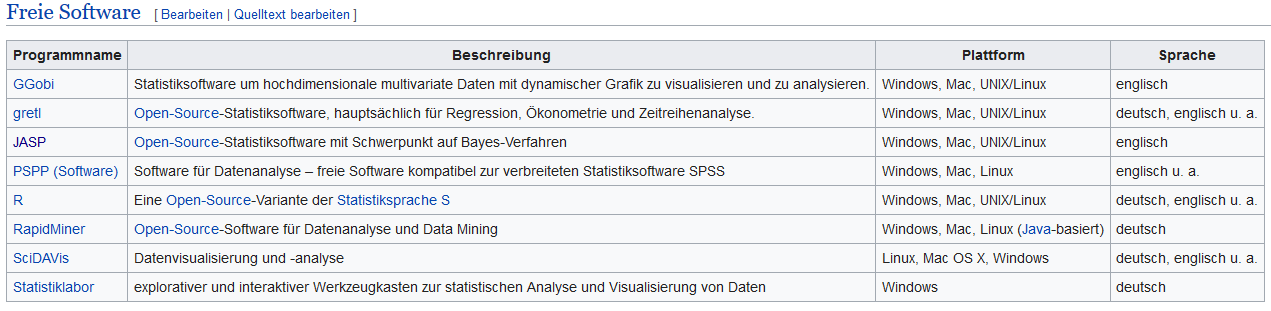
\includegraphics[width=0.70000\textwidth]{Images/FreieStatProgs.PNG}
\caption{\textbf{Abbildung 2}: frei verfügbare Statistikprogramme}
\end{figure}

Proprietäre Software:

\begin{figure}
\centering
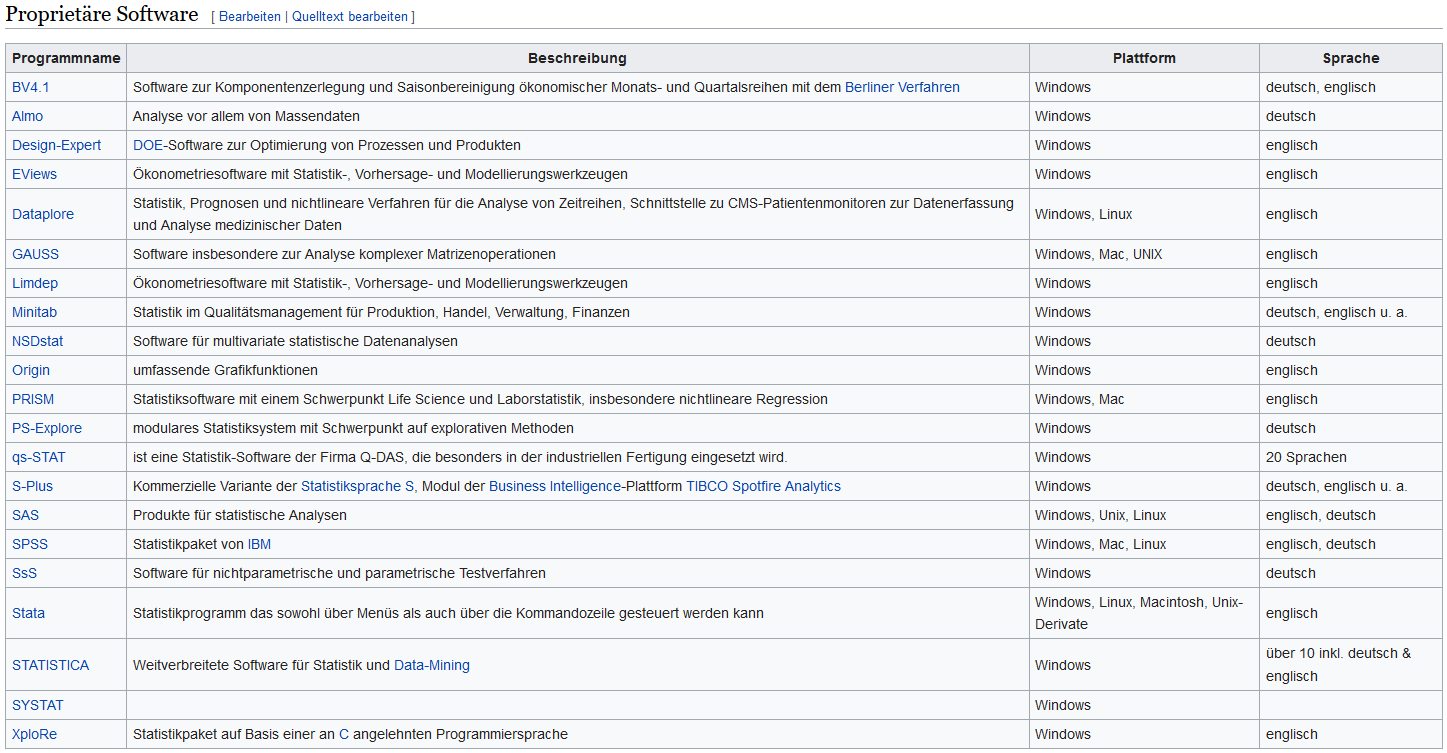
\includegraphics[width=0.70000\textwidth]{Images/ProprietaereStatProgs.PNG}
\caption{\textbf{Abbildung 3}: kostenpflichtige Statistikprogramme}
\end{figure}

Mit Stand November 2018 war laut Tiobe\footnote{\href{https://www.tiobe.com/}{TIOBE
  Programming Community Index}} R an 14 Stelle - 3 Stellen vor Matlab!
SPSS ist in der aktuellen Bewertungsliste nicht angeführt. Der
Nutzungsverlauf von R seit 2010 lässt vermuten, dass R auch in den
kommenden Jahren an Bedeutung für die statistische Analyse beibehält,
wenn nicht noch wesentlich weiterentwickelt.

\begin{figure}
\centering
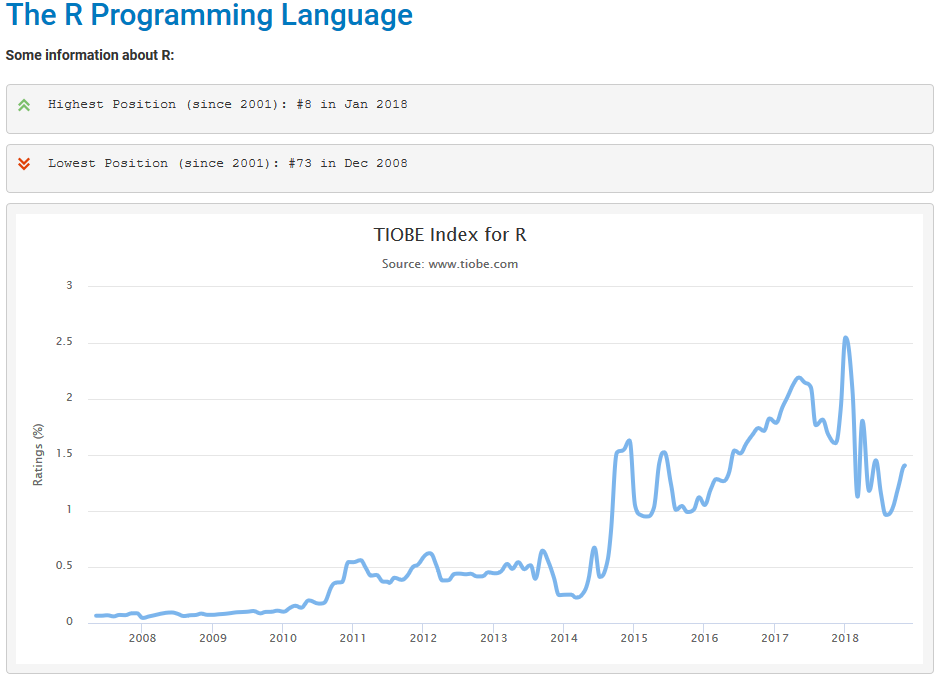
\includegraphics[width=0.50000\textwidth]{Images/TiobeRVerlauf.PNG}
\caption{\textbf{Abbildung 4}: Verlauf des
\href{https://www.tiobe.com/tiobe-index/}{TIOBE-Index} für R seit 2008
(the ratings are calculated by counting hits of the most popular search
engines. The number of hits determines the ratings of a language. The
counted hits are normalized for each search engine for all languages in
the list. In other words, all languages together have a score of
100\%.)}
\end{figure}

Zusätzlich zu dieser Liste gibt es noch viele weitere Anwendungen, die
zum Teil für ganz spezielle Analysetechniken maßgeschneidert wurden -
falls erforderlich einfach im Web danach suchen.

\paragraph{JAMOVI}\label{jamovi}
\addcontentsline{toc}{paragraph}{JAMOVI}

Ist ein Computerprogramm zur Datenanalyse und Durchführung von
statistischen Tests.

\begin{figure}
\centering
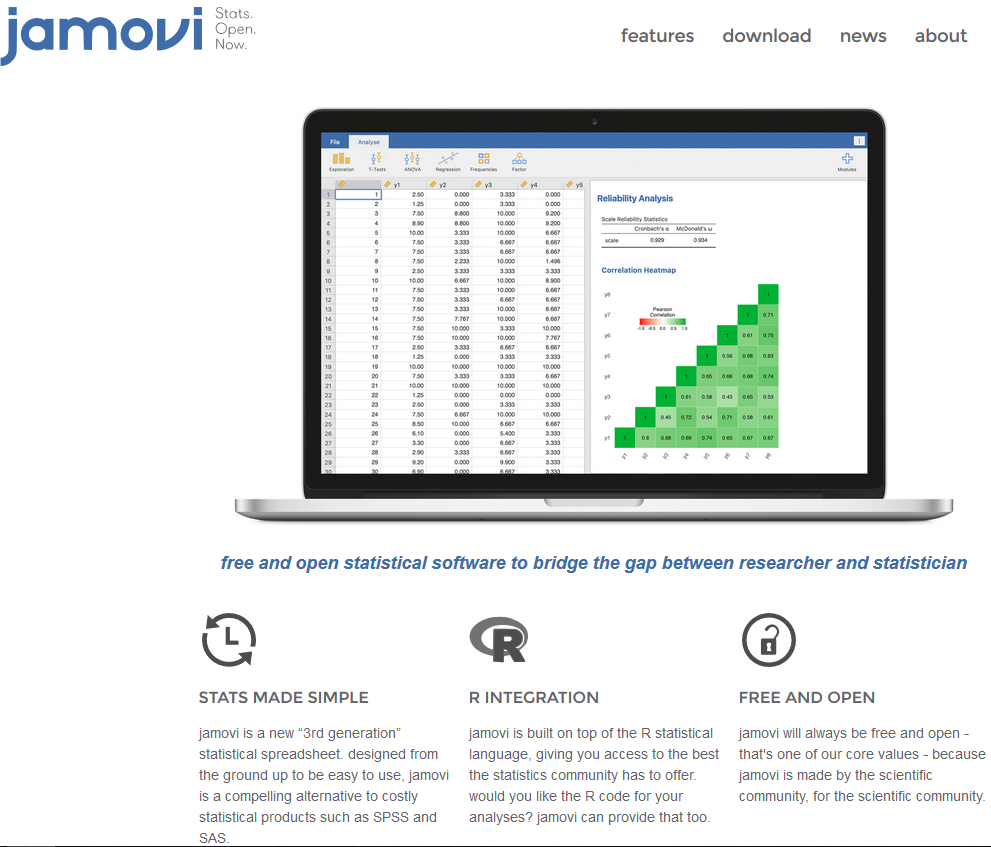
\includegraphics[width=0.50000\textwidth]{Images/JAMOVI.PNG}
\caption{\textbf{Abbildung 5}: Kurzbeschreibung von
\href{https://www.jamovi.org/}{JAMOVI}}
\end{figure}

Jamovi benutzt für die statistischen Auswertungen R. Damit bietet sich
diese Programm auch an, bei Bedarf zwischen der bequemen Benutzung von
JAMOVI und einer ins Detail gehenden Weiterentwicklung von
JAMOVI-Programmen zu wechseln. Die Voraussetzungen um problemlos
zwischen R und JAMOVI zu wechseln bietet das Paket \emph{jmv}. Um den in
JAMOVI verwendeten R Code sichtbar zu machen, ist folgende Einstellung
in JAMOVI zu wählen:

\begin{figure}
\centering
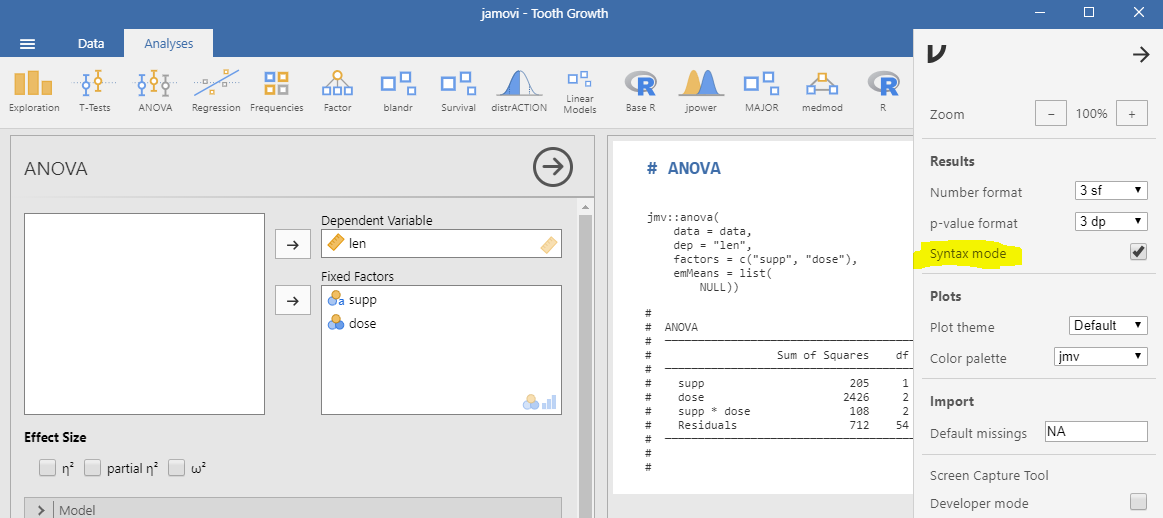
\includegraphics[width=0.50000\textwidth]{Images/01_JAMOVI_RSyntax.PNG}
\caption{\textbf{Abbildung 6}: Darstellung des R-Codes in JAMOVI}
\end{figure}

Kopiert man den Codeteil von JAMOVI nach R, kann dieser
bearbeitet/erweitert werden:

\begin{Shaded}
\begin{Highlighting}[]
  \KeywordTok{rm}\NormalTok{(}\DataTypeTok{list =} \KeywordTok{ls}\NormalTok{())}
  \ControlFlowTok{if}\NormalTok{ (}\OperatorTok{!}\KeywordTok{require}\NormalTok{(}\StringTok{"pacman"}\NormalTok{)) }\KeywordTok{install.packages}\NormalTok{(}\StringTok{"pacman"}\NormalTok{)}
\NormalTok{  pacman}\OperatorTok{::}\KeywordTok{p_load}\NormalTok{(here, jmv, xtable)}
  \KeywordTok{options}\NormalTok{(}\DataTypeTok{digits=}\DecValTok{3}\NormalTok{)}
  
\NormalTok{  DatenFile <-}\StringTok{ "/Heart Rate.csv"}
\NormalTok{  D2L       <-}\StringTok{ }\KeywordTok{paste0}\NormalTok{(}\KeywordTok{here}\NormalTok{(}\StringTok{"Data"}\NormalTok{), DatenFile)}
\NormalTok{  data      <-}\StringTok{ }\KeywordTok{read.csv}\NormalTok{(D2L, }\DataTypeTok{check.names =} \OtherTok{FALSE}\NormalTok{)}
  
\NormalTok{  jmv}\OperatorTok{::}\KeywordTok{anova}\NormalTok{(}\DataTypeTok{data =}\NormalTok{ data,}
             \DataTypeTok{dep =} \StringTok{"Heart Rate"}\NormalTok{,}
             \DataTypeTok{factors =} \KeywordTok{c}\NormalTok{(}\StringTok{"Gender"}\NormalTok{, }\StringTok{"Group"}\NormalTok{),}
             \DataTypeTok{emMeans =} \KeywordTok{list}\NormalTok{(}\OtherTok{NULL}\NormalTok{))}
  
  \CommentTok{# Erweiterung in R: Angabe der Effektgrößen in Tabelle  }
\NormalTok{  jmv}\OperatorTok{::}\KeywordTok{anova}\NormalTok{(}\DataTypeTok{data =}\NormalTok{ data,}
             \DataTypeTok{dep =} \StringTok{"Heart Rate"}\NormalTok{,}
             \DataTypeTok{factors =} \KeywordTok{c}\NormalTok{(}\StringTok{"Gender"}\NormalTok{, }\StringTok{"Group"}\NormalTok{),}
             \DataTypeTok{emMeans =} \KeywordTok{list}\NormalTok{(}\OtherTok{NULL}\NormalTok{),}
             \DataTypeTok{effectSize =} \KeywordTok{c}\NormalTok{(}\StringTok{'eta'}\NormalTok{, }\StringTok{'partEta'}\NormalTok{, }\StringTok{'omega'}\NormalTok{)) }\CommentTok{# Diese Zeile wurde in R hinzugefügt}
\end{Highlighting}
\end{Shaded}

\paragraph{JASP}\label{jasp}
\addcontentsline{toc}{paragraph}{JASP}

Ist ebenfalls ein Computerprogramm zur Datenanalyse und Durchführung von
statistischen Tests. JASP hat einen ähnlichen Funktionsumfang wie
JAMOVI. Als Besonderheit kann gelten, dass die meisten Funktionen neben
der üblichen (``frequentistischen'') Form auch in einer zweiten Form,
basierend auf der \emph{bayesschen Statistik}, verfügbar sind. Der
Funktionsumfang kann - wie auch bei JAMOVI - durch Module erweitert
werden.

\begin{figure}
\centering
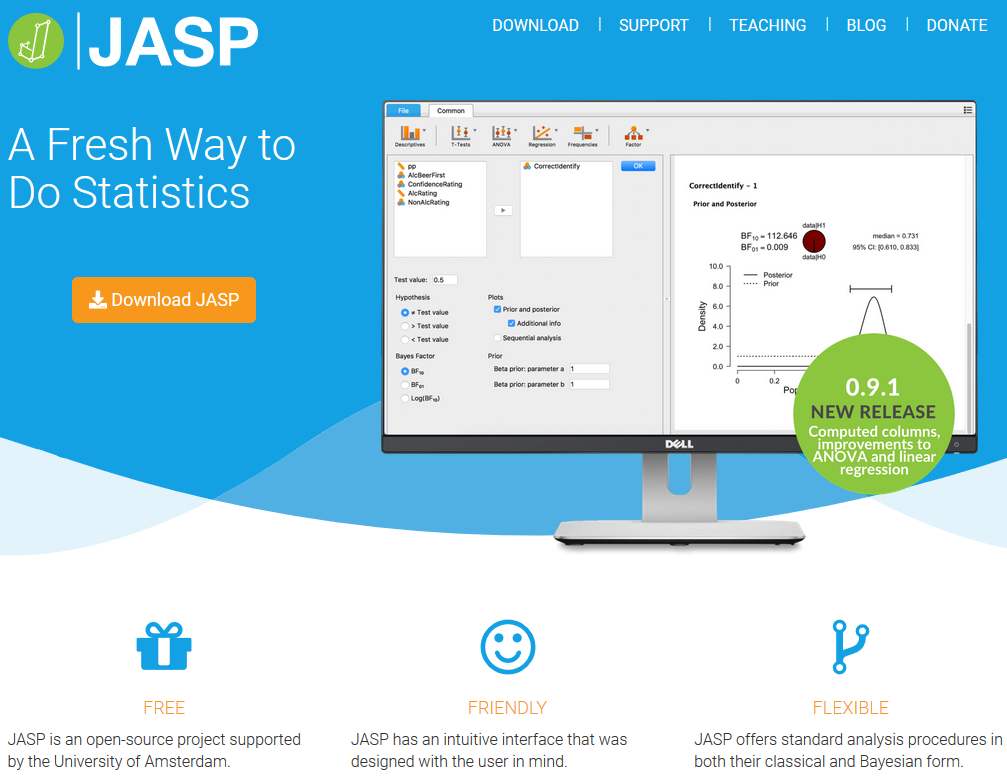
\includegraphics[width=0.50000\textwidth]{Images/JASP.PNG}
\caption{\textbf{Abbildung 7}: Kurzbeschreibung von
\href{https://jasp-stats.org/}{JASP}}
\end{figure}

Bei JASP sind neben der Bayesschen Statistik auch die verfügbaren
Datensätze für den Einstieg in die Nutzung dieses Programm
erwähnenswert. Sortiert nach Themenbereichen und referenziert nach
Herkunft kann man einerseits mit den entsprechenden Verfahren
experimentieren und gegebenenfalls auch noch in der Literatur
nachschlagen - welche eben die gleichen Datensätze zur Erklärung der
Verfahren verwendet. Man kann diese Daten aber auch exportieren und in
JAMOVI verwenden!

\section[\textbf{R}Studio]{\texorpdfstring{\textbf{R}Studio\footnote{\href{https://de.wikipedia.org/wiki/RStudio}{RStudio
  Beschreibung Wikipedia}}}{RStudio}}\label{rstudio5}

\href{https://www.rstudio.com/}{RStudio} ist eine vom Unternehmen
RStudio, Inc. angebotene, integrierte Entwicklungsumgebung und grafische
Benutzeroberfläche für die statistische Programmiersprache R. Bei
RStudio handelt es sich um eine IDE\footnote{\textbf{I}ntegrated
  \textbf{D}evelopment \textbf{E}nvironment}-Anwendung, ein Begriff den
man häufig bei der Beschreibung von RStudio verwendet.

RStudio ist sowohl als lokale Desktop-Version als auch als
Server-Version mit gleichem Layout verfügbar. Die Umgebung teilt sich in
vier Fenster (Panes), in denen:

\begin{itemize}
\tightlist
\item
  eines für die Erstellung von Skripten genutzt wird,
\item
  ein anderes als Kommandozeile mit Output des Programmiercodes und
\item
  ein weiteres für die Anzeige von Objekten in der Arbeitsumgebung.
\item
  In einem vierten Bereich lassen sich mit Reitern grafischer Output,
  eine Paketverwaltung, das Ordnerverzeichnis und mehr anzeigen.
\end{itemize}

RStudio bietet eine umfangreiche Entwicklungsumgebung und ermöglicht
eine Vielzahl sehr hilfreicher Funktionalitäten, wie:

\begin{itemize}
\tightlist
\item
  Autovervollständigung, automatische Einrückungen, Syntaxhervorhebung.
\item
  Code-Faltung.
\item
  integrierte Hilfe und Informationen zu Objekten in der
  Arbeitsumgebung.
\item
  Datensätze betrachten und bearbeiten.
\item
  Zusammenfassen von Skripten, Daten und weitere Dateien zu Projekten
  (.Rproj), was die Zusammenarbeit erleichtert, zumal eine
  Versionsverwaltung mit Git enthalten ist.
\end{itemize}

Mit Hilfe der Paketverwaltung lassen sich Pakete installieren und laden.
Die Erstellung von Berichten mit Hilfe von \emph{knitr} oder
\emph{Sweave} kann aus RStudio heraus erfolgen. Ein grafischer Debugger
ist enthalten. Zudem kann Code in C, C++ oder Fortran kompiliert werden
und direkt eingebunden werden.

Für beide Ausführungen (Desktop, Server) von RStudio kann auch eine
kommerzielle Variante erworben werden, die Support einschließt. Mit der
kommerziellen Serverversion können mehrere Sitzungen parallel laufen und
unterschiedliche Versionen von R verwendet werden. Außerdem sind das
Teilen von Projekten und das Ressourcenmanagement einfacher.

\subsection*{Aufbau von RStudio}\label{aufbau-von-rstudio}
\addcontentsline{toc}{subsection}{Aufbau von RStudio}

Beim Erststart von RStudio werden drei Fenster angezeigt. Für die
effiziente Entwicklung von R-Programmen verwendet man einen Editor,
welcher im RStudio integriert ist. Die Verwendung des Editors öffnet ein
viertes Fenster. Diese vier Fenster bilden im Allgemeinen das
Arbeitsumfeld mit RStudio.

\begin{enumerate}
\def\labelenumi{\arabic{enumi}.}
\tightlist
\item
  Konsole
\item
  Environment
\item
  Files
\item
  Source
\end{enumerate}

Die standardmäßige Anordnung und Anzeige von Details innerhalb der
Fenster kann durch den Benutzer angepasst werden. Details dazu werden
bei den jeweiligen Kapiteln besprochen.

\subsection*{R-Syntax}\label{r-syntax}
\addcontentsline{toc}{subsection}{R-Syntax}

In verschiedenen Programmiersprachen werden z.B. Groß- und
Kleinschreibung, Dezimaltrennzeichen, Sonderzeichen etc. unterschiedlich
definiert. Für R gelten folgende (grundlegende) Regeln:

\begin{itemize}
\tightlist
\item
  R unterscheidet zwischen Groß- und Kleinschreibung.
\item
  Dezimaltrennzeichen: Punkt statt Komma.
\item
  Keine Leerzeichen in Objektnamen, besser: my.object, my\_object oder
  MyObject usw.
\item
  Keine arithmetischen Operatoren (+,-,/) in Objektnamen.
\item
  Erstes Zeichen eines Objektnamens muss ein Buchstabe sein.
\item
  Befehle dürfen über mehrere Zeilen gehen.
\item
  Alles, was existiert, ist ein Objekt.
\end{itemize}

\subsection*{Kommandozeile (Befehlszeile,
Console)}\label{kommandozeile-befehlszeile-console}
\addcontentsline{toc}{subsection}{Kommandozeile (Befehlszeile, Console)}

Die \href{https://de.wikipedia.org/wiki/Kommandozeile}{Kommandozeile},
Befehlszeile (command-line interface, CLI), oft auch als Konsole oder
Terminal bezeichnet, ist ein Eingabebereich (interface) für die
Steuerung einer Software, der typischerweise (aber nicht zwingend) im
Textmodus abläuft. Die Kommandos oder Befehle werden als Zeichenketten
über die Tastatur eingegeben. Die Ausführung der Befehle wird meist
direkt aus der Zeile durch zusätzlich angegebene Parameter gesteuert
(Kommandozeilenparameter).

Ein Kommandozeilenprogramm läuft typischerweise mit den gegebenen
Parametern einmal ab, bevor eine erneute Befehlseingabe möglich ist. Ein
automatisiertes Abarbeiten mehrerer Kommandos nennt man
Stapelverarbeitung (batch).

In die Kommandozeile von RStudio können Variablendefinitionen,
Berechnungen/Funktionen, sowie der Aufruf von Hilfefunktionen direkt
eingegeben und ausgeführt werden. Die folgenden Beispiele zeigen die
Auswirkungen von direkten Eingaben in der Konsole:

\begin{Shaded}
\begin{Highlighting}[]
\DecValTok{2} \OperatorTok{+}\StringTok{ }\DecValTok{2}
\KeywordTok{help}\NormalTok{(mean)}
\NormalTok{?mean}
\NormalTok{Var1 <-}\StringTok{ }\KeywordTok{c}\NormalTok{(}\DecValTok{2}\NormalTok{,}\DecValTok{3}\NormalTok{,}\DecValTok{4}\NormalTok{)}
\KeywordTok{mean}\NormalTok{(Var1)}
\end{Highlighting}
\end{Shaded}

\subsection*{Mathematische
Operatoren/Funktionen}\label{mathematische-operatorenfunktionen}
\addcontentsline{toc}{subsection}{Mathematische Operatoren/Funktionen}

Arithmetische und logische Operatoren in R sind in nachfolgender Tabelle
definiert. Des weiteren findet man auszugsweise ein paar mathematische
Funktionen, anhand deren das Prinzip eines Funktionsaufrufes
verdeutlicht werden. Funktionen haben in R folgende Eigenschaften:

\begin{itemize}
\tightlist
\item
  jede Funktion hat einen Namen (z.B. sin für die Sinusfunktion, aov für
  Fit an Analysis of Variance Model, \ldots{})
\item
  eine Funktion kann unter Umständen ohne Parameter (z.B.
  \emph{getwd()}), oder mit einem oder mehrerern Parametern aufgerufen
  werden (z.B. \emph{mean(x)}, \emph{mean(x, na.rm = TRUE)}.
\item
  Für Funktionen, bei denen die Übergabe von Parametern notwendig ist
  (z.B. \emph{mean()}), ist folgendes zu beachten (gib in der Console
  den Befehl \emph{?mean} ein - beachte das Help-Fenster).

  \begin{itemize}
  \tightlist
  \item
    In Klammern stehende Parameter die keine Bezeichnung aufweisen (bei
    der Funktion \emph{mean} das \emph{x}), sind zwingende Angaben für
    den Aufruf der Funktion.
  \item
    Bei Parametern, die mit einem Namen versehen sind, handelt es sich
    um optionale Parameter. Diese müssen beim Aufruf der Funktion nicht
    angegeben werden. In diesem Fall werden die in der Hilfe
    ersichtlichen Standardwerte verwendet.
  \item
    Sollten die Standardwerte nicht verwendet werden, sind diese beim
    Aufruf der Funktion mit entsprechenden Werten zu versehen - wie z.B.
    bei \emph{mean(x, trim = .2, na.rm = TRUE)}.
  \item
    Wird die Reihenfolge laut Beschreibung der Funktion in der
    Hilfeseite eingehalten, können die Namen der Parameter weggelassen
    werden. Kopiere bitte zeilenweise den nachfolgenden Code in die
    Konsole und diskutieren die Ergebnisse.
  \end{itemize}
\end{itemize}

\begin{Shaded}
\begin{Highlighting}[]
\NormalTok{x <-}\StringTok{ }\KeywordTok{c}\NormalTok{(}\KeywordTok{rpois}\NormalTok{(}\DataTypeTok{n =} \DecValTok{50}\NormalTok{, }\DataTypeTok{lambda =} \DecValTok{10}\NormalTok{), }\DecValTok{100}\NormalTok{, }\OtherTok{NA}\NormalTok{, }\OtherTok{NA}\NormalTok{)}
\KeywordTok{hist}\NormalTok{(x)}
\KeywordTok{mean}\NormalTok{(x)}
\KeywordTok{mean}\NormalTok{(x, }\DataTypeTok{na.rm =} \OtherTok{TRUE}\NormalTok{)}
\KeywordTok{mean}\NormalTok{(x, }\DataTypeTok{na.rm =} \OtherTok{TRUE}\NormalTok{, }\DataTypeTok{trim =}\NormalTok{ .}\DecValTok{1}\NormalTok{)}
\KeywordTok{mean}\NormalTok{(x, }\OtherTok{TRUE}\NormalTok{, .}\DecValTok{1}\NormalTok{)}
\KeywordTok{mean}\NormalTok{(x, .}\DecValTok{1}\NormalTok{, }\OtherTok{TRUE}\NormalTok{)}
\end{Highlighting}
\end{Shaded}

\begin{figure}
\centering
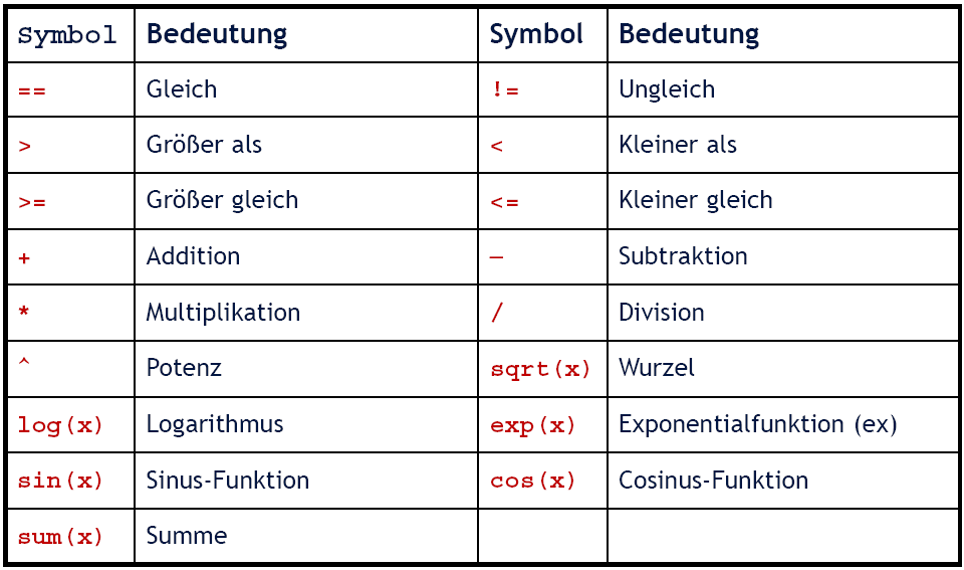
\includegraphics[width=0.50000\textwidth]{Images/R_Operatoren.PNG}
\caption{\textbf{Tabelle 1}: Operatoren und Funktionen}
\end{figure}

\subsection*{Hilfe in RStudio}\label{hilfe-in-rstudio}
\addcontentsline{toc}{subsection}{Hilfe in RStudio}

Mit der Installation von RStudio wird automatisch auch eine
Dokumentation der verfügbaren Funktionen zur Verfügung gestellt. Dieses
Hilfe-System kann auf unterschiedlichste Arten angesprochen werden.
Folgende Möglichkeiten sind im RStudio gegeben:

\begin{itemize}
\tightlist
\item
  über die \emph{Console} mit folgenden Befehlen
\end{itemize}

\begin{Shaded}
\begin{Highlighting}[]
\KeywordTok{help.search}\NormalTok{(}\StringTok{"mean"}\NormalTok{)}
\KeywordTok{help}\NormalTok{(}\StringTok{"mean"}\NormalTok{)}
\NormalTok{?mean}
\end{Highlighting}
\end{Shaded}

\begin{itemize}
\tightlist
\item
  über das \emph{Help}-Menü
\item
  über das \emph{Files}-Pane im Reiter \emph{Help}
\end{itemize}

Darüber hinaus gibt es noch die Möglichkeit, eine der unzähligen
Helpseiten im Internet in Anspruch zu nehmen. Eine Empfehlung, welche
Hilfeseite(n) am besten sind ist schwer zu geben - durch Erfahrung und
persönlichen Vorlieben werden sich schnell ein paar Seiten als hilfreich
bewähren. Zum Einstieg nachfolgend ein paar Seiten die ich persönlich
immer wieder verwende:

\begin{itemize}
\tightlist
\item
  \href{https://www.r-project.org/help.html}{R-project}
\item
  \href{http://www.cookbook-r.com/}{Cookbook for R}
\item
  \href{https://www.statmethods.net/interface/help.html}{Quick-R}
\item
  \href{https://www.rdocumentation.org/packages/utils/versions/3.5.1/topics/help}{RDocumentation}
\item
  \href{https://support.rstudio.com/hc/en-us}{RStudio Support}
\item
  u.v.m.
\end{itemize}

\subsubsection*{Online-Lernprogramme}\label{online-lernprogramme}
\addcontentsline{toc}{subsubsection}{Online-Lernprogramme}

Eine weitere (unerschöpfliche) Quelle um R effizient und schnell zu
erlernen sind entsprechende Online-Kurse. Einerseits gibt es über
YouTube bereits viele Tutorials (die mehr oder weniger hilfreich
sind/sein können). Andererseits haben sich aber bereits einige
Universitäten und Firmen darauf spezialisiert, qualitativ hochwertige
Online-Tutorials und Webinars zur Verfügung zu stellen. Viele davon sind
noch kostenlos. Auch hier ist es schwierig eine punktuelle Empfehlung
abzugeben. Nachfolgend eine kurze (und daher sicher unvollständige)
Liste von Anbietern, die ich zumindest zum Teil selbst ausprobiert und
als gut empfunden habe:

\begin{itemize}
\tightlist
\item
  \href{https://www.datacamp.com/}{DataCamp}.
\item
  \href{https://www.coursera.org/}{coursera}.
\item
  \href{https://www.rstudio.com/online-learning/}{RStudio Online
  Learning}.
\item
  \href{https://www.udemy.com/r-programming/}{Course}.
\item
  \href{https://www.statmethods.net/r-tutorial/index.html}{Quick-R
  Tutorials}.
\end{itemize}

\subsubsection*{Verwendung der Konsole (Aufgabe
1)}\label{verwendung-der-konsole-aufgabe-1}
\addcontentsline{toc}{subsubsection}{Verwendung der Konsole (Aufgabe 1)}

Berechne in der Konsole die Ergebnisse folgender Ausdrücke und prüfe das
Ergebnis auf Korrektheit:

\begin{enumerate}
\def\labelenumi{\alph{enumi}.}
\tightlist
\item
  \((3 + 4 - 5) * 9\)
\item
  \(\frac{99}{33}\)
\item
  \((\sqrt{2})^2\)
\item
  \(e^{3+4}\)
\end{enumerate}

Gib nachfolgende Befehle ein und diskutiere das Ergebnis:

\begin{enumerate}
\def\labelenumi{\alph{enumi}.}
\tightlist
\item
  \(5 = 7\)
\item
  \(5 == 7\)
\item
  \(5*5 >= 6*4\)
\item
  \(\sqrt{3} \neq cos(17)\)
\end{enumerate}

Die Lösungen zu den Beispielen findest du am Ende dieses Dokumentes.

\subsubsection*{Wiederverwendung von Befehlszeilen - die
Command-History}\label{wiederverwendung-von-befehlszeilen---die-command-history}
\addcontentsline{toc}{subsubsection}{Wiederverwendung von Befehlszeilen
- die Command-History}

Durch die Verwendung der Pfeiltasten (\(\uparrow\) und \(\downarrow\))
können Sie bereits eingegeben Befehle in der Kommandozeile aus der
Historie abrufen. Die Historie ist auch über das Environment Fenster im
Tab \emph{History} verfügbar. Durch Markieren einzelner oder mehrerer
Zeilen im History-Fenster und anschließender Eingabetaste, werden diese
Befehle in die Kommandozeile übernommen und können dort nochmals
ausgeführt werden.

\subsubsection*{Weitere Eigenschaften der Console
Pane}\label{weitere-eigenschaften-der-console-pane}
\addcontentsline{toc}{subsubsection}{Weitere Eigenschaften der Console
Pane}

Neben der Ausgabe von Ergebnissen werden in der Console-Pane auch
Hinweise, Warnungen und Fehler die während der Ausführung eines
Programmes, bzw. dem Laden/Aktualisieren von Packages ausgegeben werden
angezeigt. Dabei ist vor allem bei den Meldungen, die während des
Ladens/Aktualisierens von Packages angezeigt werden, besondere
Aufmerksamkeit angebracht. Alle Meldungen, also rein informative wie
auch Fehlermeldungen, werden in \(\color{red}{\text{rot}}\) angezeigt.
Da häufig sehr viele Meldungen (sehr schnell) über die Console laufen,
übersieht man leicht Fehlermeldungen. Daher ist es vor allem bei langen
Meldungen zu empfehlen, die Gesamte Meldungsliste sorgfältig zu
kontrollieren.

\subsection*{Terminal-Fenster}\label{terminal-fenster}
\addcontentsline{toc}{subsection}{Terminal-Fenster}

Das Terminalfenster bietet die Möglichkeit, direkt auf die
Systemumgebung zuzugreifen. über die Systemumgebung kann man z.B.:

\begin{itemize}
\tightlist
\item
  Fernzugriffe (remote logins) ausführen.
\item
  lang dauernde Berechnungen im Hintergrund starten.
\item
  Fortgeschrittene Programmkontrolle starten.
\item
  Administration eines RStudio-Servers durchführen.
\item
  etc.
\end{itemize}

\subsection*{R-Markdown-Fenster}\label{r-markdown-fenster}
\addcontentsline{toc}{subsection}{R-Markdown-Fenster}

\href{https://de.wikipedia.org/wiki/Markdown}{R-Markdown Beschreibung}
ist eine vereinfachte Auszeichnungssprache, mit dem Ziel Dokumente zu
erstellen, in dem sowohl Text, wie auch R-Code sein kann. Markdown ist
eng an HTML angelehnt, aber bei weitem kein Ersatz dafür. Wesentliche
Vorteile von Markdown sind:

\begin{itemize}
\tightlist
\item
  Sehr leicht erlernbar.
\item
  Forschung wird reproduzierbar.
\item
  Leichterer Austausch von Analyseergebnissen und der zugehörigen
  Dokumentation.
\item
  Beim Erstellen (``knit'') wird der Code ausgeführt und mit den
  Beschreibungen zusammen angezeigt.
\item
  Das kombinierte Dokument kann als Word-, HTML- oder PDF-Datei
  erstellt.
\end{itemize}

Neben der Nutzung als Software-Dokumentationswerkzeug bietet Markdown
auch eine einfache Möglichkeit, einen Forschungsprozess durchgehend
abzubilden und Inhalte mit fortlaufender Evaluierung während der
Datenerhebung zu verbinden (Stichwort \emph{sanity-check}).

\textbf{Ein Beispiel für die Nutzung von Markdown sind sämtliche
Unterlagen dieser LV!}

\begin{center}\rule{0.5\linewidth}{\linethickness}\end{center}

\subsection*{Lösungen}\label{losungen}
\addcontentsline{toc}{subsection}{Lösungen}

\hypertarget{aufgabe-1}{\subsubsection*{Aufgabe 1}\label{aufgabe-1}}
\addcontentsline{toc}{subsubsection}{Aufgabe 1}

\begin{Shaded}
\begin{Highlighting}[]
\KeywordTok{rm}\NormalTok{(}\DataTypeTok{list =} \KeywordTok{ls}\NormalTok{())}
\ControlFlowTok{if}\NormalTok{ (}\OperatorTok{!}\KeywordTok{require}\NormalTok{(}\StringTok{"pacman"}\NormalTok{)) }\KeywordTok{install.packages}\NormalTok{(}\StringTok{"pacman"}\NormalTok{)}
\NormalTok{pacman}\OperatorTok{::}\KeywordTok{p_load}\NormalTok{(here)}
\CommentTok{# Berechnungen}
\NormalTok{(}\DecValTok{3} \OperatorTok{+}\StringTok{ }\DecValTok{4} \OperatorTok{+}\StringTok{ }\DecValTok{5}\NormalTok{) }\OperatorTok{*}\StringTok{ }\DecValTok{9}
\DecValTok{99} \OperatorTok{/}\StringTok{ }\DecValTok{33}
\KeywordTok{sqrt}\NormalTok{(}\DecValTok{2}\NormalTok{)}\OperatorTok{^}\DecValTok{2}
\KeywordTok{exp}\NormalTok{(}\DecValTok{3}\OperatorTok{+}\DecValTok{4}\NormalTok{)}
\CommentTok{# Logische Vergleiche}
\DecValTok{5}\NormalTok{ =}\StringTok{ }\DecValTok{7}
\DecValTok{5} \OperatorTok{==}\StringTok{ }\DecValTok{7}
\DecValTok{5}\OperatorTok{*}\DecValTok{5} \OperatorTok{>=}\StringTok{ }\DecValTok{6}\OperatorTok{*}\DecValTok{4}
\KeywordTok{sqrt}\NormalTok{(}\DecValTok{3}\NormalTok{) }\OperatorTok{!=}\StringTok{ }\KeywordTok{cos}\NormalTok{(}\DecValTok{17}\NormalTok{)}
\end{Highlighting}
\end{Shaded}

\section{Source-Pane}\label{source-pane}

Der Source-Pane, oder auch Editor, ist ein äußerst hilfreiches
Instrument bei der Erstellung von Programmen. Im Gegensatz zur Konsole
ist es im Editor möglich, mehrere Befehle hintereinander aufzuzeichnen
und diese dann nach Wunsch einzeln, blockweise oder gesamt auszuführen.
Da in den meisten Füllen die Analyse von Daten aus mehreren/vielen
hintereinander folgenden Arbeitsschritten (laden der Daten, Berechnung
der deskriptiven Statistik, Erstellung von Graphen, inferenzstatistische
Auswertung, etc.), ist die Programmierung ohne Editor undenkbar.

Der mit RStudio zur Verfügung gestellte Editor hat neben der Möglichkeit
Programmcode aufzuzeichnen und zu speichern eine Fälle weiterer
Möglichkeiten. Die wichtigsten Eigenschaften für einen Start in die
R-Programmierung werden in den folgenden Kapiteln kurz angesprochen.

\subsection*{Dateitypen}\label{dateitypen}
\addcontentsline{toc}{subsection}{Dateitypen}

Der Editor bietet für die Erstellung von Dokumenten verschiedene
Fiel-typen an:

\begin{figure}
\centering
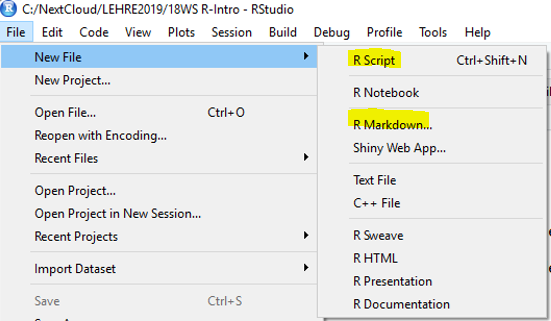
\includegraphics[width=0.50000\textwidth]{Images/03_R_File_Types.PNG}
\caption{\textbf{Abbildung 8}: Dateitypen R}
\end{figure}

\subsubsection*{R Script}\label{r-script}
\addcontentsline{toc}{subsubsection}{R Script}

Das meist verwendete und für den Einstieg wesentliche Dokument ist das R
Script. Geöffnete wird ein leeres Arbeitsblatt in welchem zeilenweise
die Befehle und Funktionen von R eingefügt werden. Der Editor bietet
aber darüber hinaus eine Vielzahl an weiterer Möglichkeiten, wie z.B.:

\begin{itemize}
\tightlist
\item
  Code-Complete Funktion
\item
  Keyboard Shortcuts
\item
  Code Snippets
\item
  Extract Funktion
\item
  Suchfunktionen
\item
  Code Ausführung
\item
  Traceback und Debugging
\item
  Kommentare und Dokumentation von Code, oder Codeteilen
\end{itemize}

Anwendung und Eigenschaften dieser Möglichkeiten werden im folgenden
besprochen.

\subsubsection*{R-Markdown}\label{r-markdown}
\addcontentsline{toc}{subsubsection}{R-Markdown}

R-Markdown ist eine Dokumentenart, mit der Textverarbeitung mit
gleichzeitiger Nutzung aller R-Funktionalitäten vereint werden.
Besondere Erwähnung findet es hier deshalb, da alle zur Verfügung
stehenden Unterlagen dieses Kurses mit R-Markdown erstellt wurden.
Sofern es zeitlich möglich ist, werden wir am Ende der Lehrveranstaltung
die Verwendung und Anwendbarkeit dieser Option besprechen.

\subsubsection*{Andere Dokumentenarten}\label{andere-dokumentenarten}
\addcontentsline{toc}{subsubsection}{Andere Dokumentenarten}

Die restlichen Arten von Dokumenten sind spezielle Formate, die eine
Einbindung von C++ und diversen Dokumentationsformaten erlauben. Zu
erwähnen wäre in diesem Zusammenhang noch die \emph{Shiny Web App}, mit
welcher man relativ einfach Benutzerschnittstellen (UI's\footnote{User
  Interfaces}) erzeugen kann. Diese Schnittstelle ist vor allem dann von
Vorteil, wenn bestimmte Programme auch für Nutzer die keinen
R-Background haben zur Verfügung gestellt werden.

\subsection*{Nützliches im Editor}\label{nutzliches-im-editor}
\addcontentsline{toc}{subsection}{Nützliches im Editor}

Im folgenden beschäftigen wir uns kurz mit einigen der hilfreichsten
Eigenschaften des RStudio-Editors.

\subsubsection*{Code completion}\label{code-completion}
\addcontentsline{toc}{subsubsection}{Code completion}

Unter \emph{code completion} versteht man die Eigenschaft des Editors,
während der Eingabe einer Funktions-, bzw. Variablennamens eine Liste
der verfügbaren Funktionen/Variablen anzuzeigen und diese auch mit dem
Tabulatur (\(\rightleftharpoons\)) zu übernehmen.

Nach wie vielen Zeichen die Liste angezeigt wird, kann über die
\emph{Global Options} im Menü \emph{Tools} eingestellt werden
(standardmäßig wird nach 3 Zeichen die Liste angezeigt).

\begin{figure}
\centering
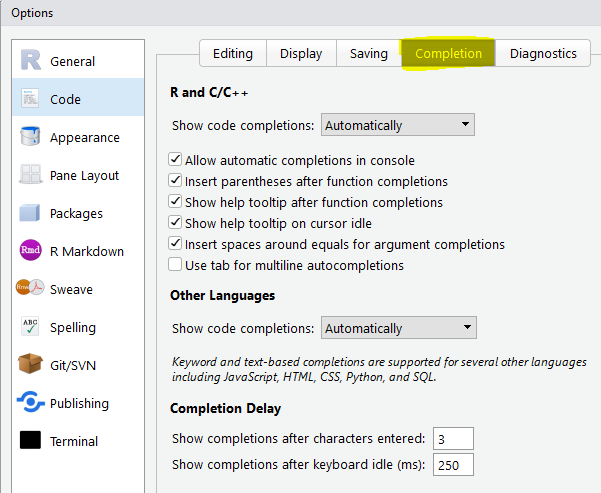
\includegraphics[width=0.50000\textwidth]{Images/03_R_CodeCompletion.PNG}
\caption{\textbf{Abbildung 9}: Einstellungen \emph{code completion} im
Menü Tools \(\rightarrow\) Global Options \(\rightarrow\) Code
\(\rightarrow\) Completion}
\end{figure}

Öffne eine neue \emph{R Script} Datei. Kopiere die erste Zeile des
nachfolgenden Codes in das Skript und führe diese aus (markieren der
Zeile mit anschließendem Drücken von \emph{Ctrl Enter}). Gib nun die
weiteren Befehlszeilen direkt in den Editor ein und beobachte den
Effekt, der sich nach der Eingabe des dritten Zeichens zeigt.

\subsubsection*{Keyboard Short-Cuts}\label{keyboard-short-cuts}
\addcontentsline{toc}{subsubsection}{Keyboard Short-Cuts}

Mit Hilfe der Keyboard-Shortcuts können Zeichen, Funktionen, etc.
schnell und einfach in das Skript eingefügt werden. Mit der
Basisinstallation wurden bereits eine Menge von Shortcuts definiert.
Eine Liste dieser Shortcuts ist durch den Shortcut \emph{Alt Shift K},
oder unter folgendem Menü zu finden:

\begin{figure}
\centering
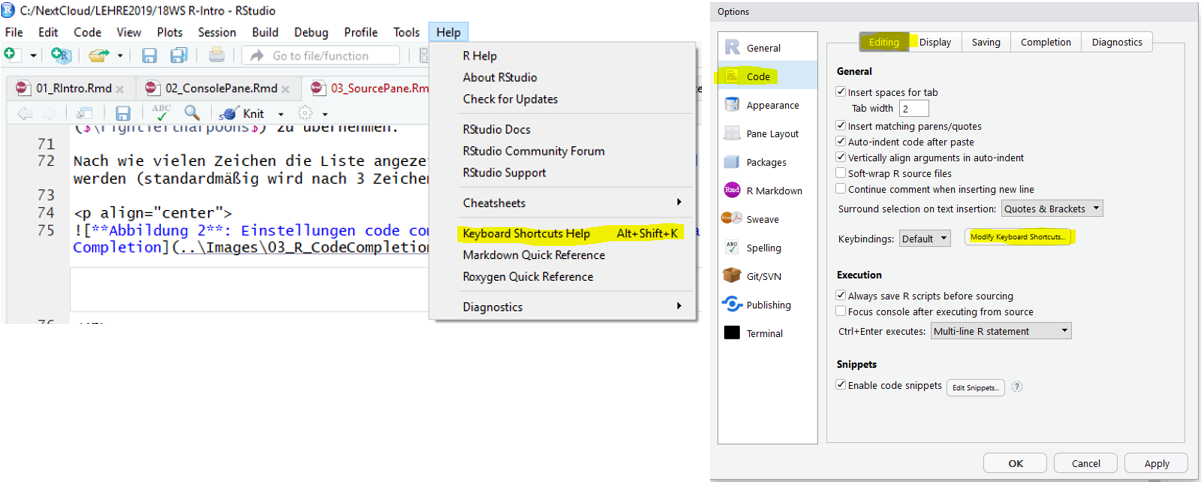
\includegraphics[width=0.70000\textwidth]{Images/03_R_ShortCuts.PNG}
\caption{\textbf{Abbildung 10}: Shortcut Liste (\emph{Alt Shift K}) und
Änderungsmöglichkeiten für Shortcuts (Tools \(\rightarrow\) Global
Options \(\rightarrow\) Code \(\rightarrow\) Editing)}
\end{figure}

Welche der Shortcuts man sich wirklich merken soll ist Geschmacksache.
Zwei sehr häufig von mir verwendete wären:

\begin{itemize}
\tightlist
\item
  Kommentar mit Ctrl Shift C
\item
  Lange Zeilen besser darstellen mit Ctrl Shift /, etc.
\end{itemize}

\subsubsection*{Code Snippets}\label{code-snippets}
\addcontentsline{toc}{subsubsection}{Code Snippets}

Neben den Shortcuts bieten auch die \emph{Snippets} eine bedeutende
Erleichterung beim Schreiben von Codes. Dabei handelt es sich um
Textmakros die häufig verwendete Codefragmente in das Skript einfügen
können. Vordefinierte Snippets können unter Tools \(\rightarrow\) Global
Options \(\rightarrow\) Code \(\rightarrow\) Edit angesehen und auch
geändert, bzw. hinzugefügt werden.

\begin{figure}
\centering
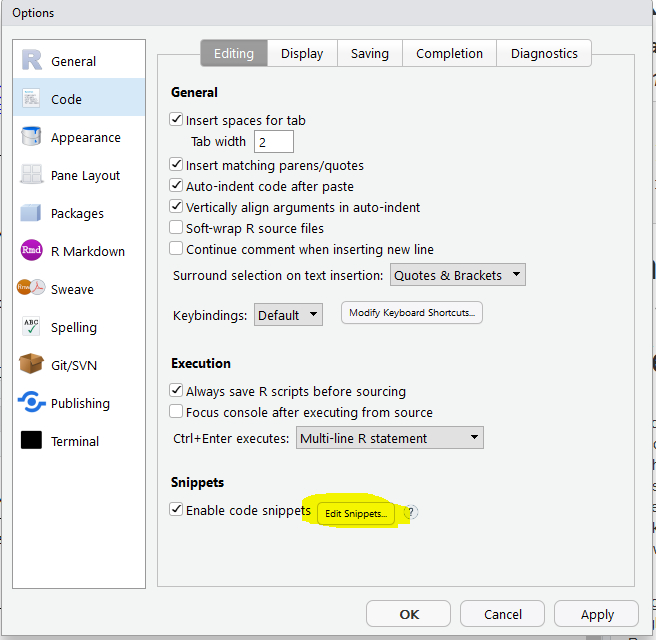
\includegraphics[width=0.50000\textwidth]{Images/03_RSnippets.PNG}
\caption{\textbf{Abbildung 11}: Snippets Definition und
Änderungsmöglichkeiten (Tools \(\rightarrow\) Global Options
\(\rightarrow\) Code \(\rightarrow\) Edit Snippets)}
\end{figure}

Wie bei der \emph{code completion} werden nach 3 eingegebenen Zeichen
die vordefinierten Snippets in einer Liste angezeigt. Die Übernahme des
Inhalts wird durch Auswahl gefolgt vom Tabulator
(\(\rightleftharpoons\)) durchgeführt. Wird z.B. \emph{fun} eingegeben,
wird automatisch folgende Liste angezeigt:

\begin{figure}
\centering
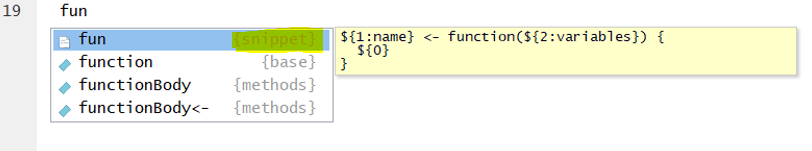
\includegraphics[width=0.70000\textwidth]{Images/03_RSnippets_Bsp.PNG}
\caption{\textbf{Abbildung 12}: Snippets Definition und
Anderungsmöglichkeiten (Tools \(\rightarrow\) Global Options
\(\rightarrow\) Code \(\rightarrow\) Edit Snippets)}
\end{figure}

Durch Wahl der entsprechenden Funktion (in diesem Fall das Snippet),
wird das Makro ausgeführt und der vordefinierte Text in den Editor
eingefügt. Probier es am besten selbst aus. Gib \emph{fun} ein, wähle
das \emph{snippet fun} und drücke die Tabulatortaste. Diskutiere das
Ergebnis.

\subsubsection*{Extract Funktion}\label{extract-funktion}
\addcontentsline{toc}{subsubsection}{Extract Funktion}

Die extract function wird vor allem dann verwendet, wenn ein selbst
geschriebener Codeteil in eine Funktion umgewandelt werden soll. Die
Vorgehensweise ist dabei denkbar einfach:

\begin{enumerate}
\def\labelenumi{\arabic{enumi}.}
\tightlist
\item
  schreibe einen Code.
\item
  markiere den Code.
\item
  wähle im Menü \(\rightarrow\) Code \(\rightarrow\) Extract Function,
  oder drücke \emph{Ctrl Alt X}.
\item
  Bennen die Funktion.
\end{enumerate}

Kopier die folgenden Zeilen in den Editor und wandle die Zeile:

\begin{enumerate}
\def\labelenumi{\arabic{enumi}.}
\tightlist
\item
  \emph{x - mean(x)} in eine Funktion mit dem Namen \emph{center} um.
\item
  \emph{x / sd(x)} in eine Funktion mit dem Namen \emph{rescale} um.
\item
  \emph{rescale(center(x))} in eine Funktion mit dem Namen
  \emph{standardize} um.
\item
  Markiere die drei Funktionen sowie die Zeilen \emph{x \textless{}-
  1:10} und \emph{standardize(x)} und drücke \emph{Ctrl Enter}
\item
  Diskutiere das Ergebnis.
\end{enumerate}

Wenn alles funktioniert hat, sollte dein Code folgendermaßen aussehen:

\subsubsection*{Suchfunktionen}\label{suchfunktionen}
\addcontentsline{toc}{subsubsection}{Suchfunktionen}

Häufig werden wir nach bestimmten Begriffen (Funktionsnamen,
Variablennamen, etc.) innerhalb unseres Codes suchen. Mit \emph{Ctrl f},
bzw. über das Menü \emph{Edit} \(\rightarrow\) \emph{Find}, wird das zur
einfachsten Sache - beachte das Suchfeld direkt unter der Symbolleiste,
sowie die Möglichkeiten für die Einschränkung der Suche (In selection,
Match case, etc.). Gleichzeitig wird damit auch die Möglichkeit gegeben,
bestimmte Suchbegriffe im Text zu ersetzen (siehe \emph{Replace} Feld).

\begin{figure}
\centering
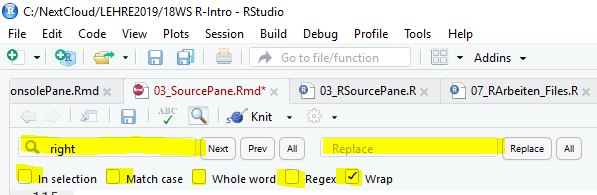
\includegraphics[width=0.50000\textwidth]{Images/03_R_SucheErsetzen.PNG}
\caption{\textbf{Abbildung 13}: Suchen und Ersetzen im geöffneten
Script}
\end{figure}

Eine überaus wertvolle Suchfunktion kann durch \emph{Ctrl Shift f}, bzw.
über das Menü \emph{Edit} \(\rightarrow\) \emph{Find in Files},
aufgerufen werden. Mit dieser Suchfunktion werden alle Files eines
bestimmten Verzeichnisses auf bestimmte Begriffe durchsucht.

\subsubsection*{Code Folding}\label{code-folding}
\addcontentsline{toc}{subsubsection}{Code Folding}

Mit \emph{code folding} kann man vor allem bei längeren Programmen sehr
gut die Übersicht von bestimmten Programmteilen behalten. Als Beispiel
kann man den soeben erzeugten Code nochmals genauer betrachten:

\begin{figure}
\centering
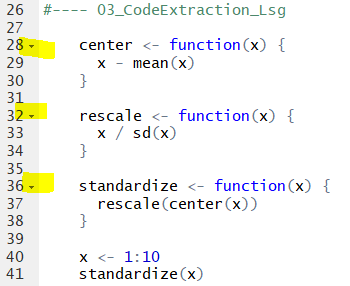
\includegraphics[width=0.30000\textwidth]{Images/03_R_CodeFoling.PNG}
\caption{\textbf{Abbildung 14}: Code Folding}
\end{figure}

Bei genauerem Hinsehen fallen einem vielleicht die schwarzen Dreiecke
direkt neben der Zeilennummerierung auf. Klickt man diese mit der Maus
an, wird entweder ein Teil des Codes auf eine Zeile reduziert
(\emph{folding}), oder falls bereits reduziert, wieder entfaltet.

Anwendung findet diese Möglichkeit vor allem bei Codeteilen, die bereits
getestet wurden und deren Einzelheiten für die weitere Entwicklung von
Code nicht von Interesse sind. Damit wird unwesentliche ausgeblendet und
die Übersicht über den relevanten Code leichter behalten.

\subsection*{Running Code}\label{running-code}
\addcontentsline{toc}{subsection}{Running Code}

Für die zeilenweise Ausführung von Code brauch man nur in der
betroffenen Zeile \emph{Ctrl Enter} drücken (die Zeile kann, aber muss
dafür nicht markiert sein). Wir die Markierung verwendet, ist darauf zu
achten, dass genau der markierte Inhalt ausgeführt wird!

Der Vorteil der Markierung liegt darin, dass nicht nur eine Zeile,
sondern markierte Bereiche (Blöcke) ausgeführt werden können.

Darüber hinaus bieten sich im RStudio die Symbolleisten für die
Ausführung von Code an:

\begin{figure}
\centering
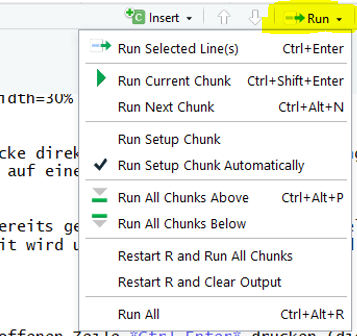
\includegraphics[width=0.30000\textwidth]{Images/03_R_RunSymbol.PNG}
\caption{\textbf{Abbildung 15}: Code Folding}
\end{figure}

\subsection*{Traceback (Debugging)}\label{traceback-debugging}
\addcontentsline{toc}{subsection}{Traceback (Debugging)}

Eine wirklich geniale Sache bei RStudio ist die integrierte Möglichkeit
des sogenannten \emph{Debugging}. Um Debugging zu demonstrieren,
verwenden wir den Codeteil aus dem Kapitel \emph{extract function}.
Bitte den nachfolgend gezeigten Code in ein neues RScript kopieren.

\begin{figure}
\centering
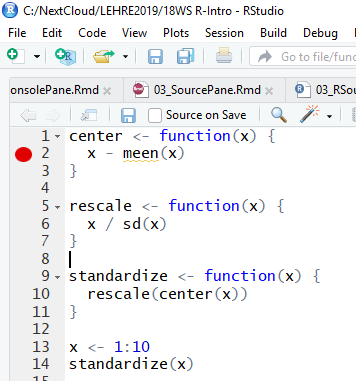
\includegraphics[width=0.30000\textwidth]{Images/03_R_Debugging.PNG}
\caption{\textbf{Abbildung 16}: Debugging in R}
\end{figure}

Führe nun folgende Schritte aus:

\begin{enumerate}
\def\labelenumi{\arabic{enumi}.}
\tightlist
\item
  Speichere den neuen Code unter den Namen \emph{03\_DebuggingDemo.R}.
\item
  Ändere in der Funktion center \emph{mean(x)} auf \emph{meen(x)} (wir
  fügen absichtlich einen Fehler ein!)
\item
  Speichere das Skript und führe es aus (mit \emph{Source} in der
  Symbolleiste)
\end{enumerate}

\begin{figure}
\centering
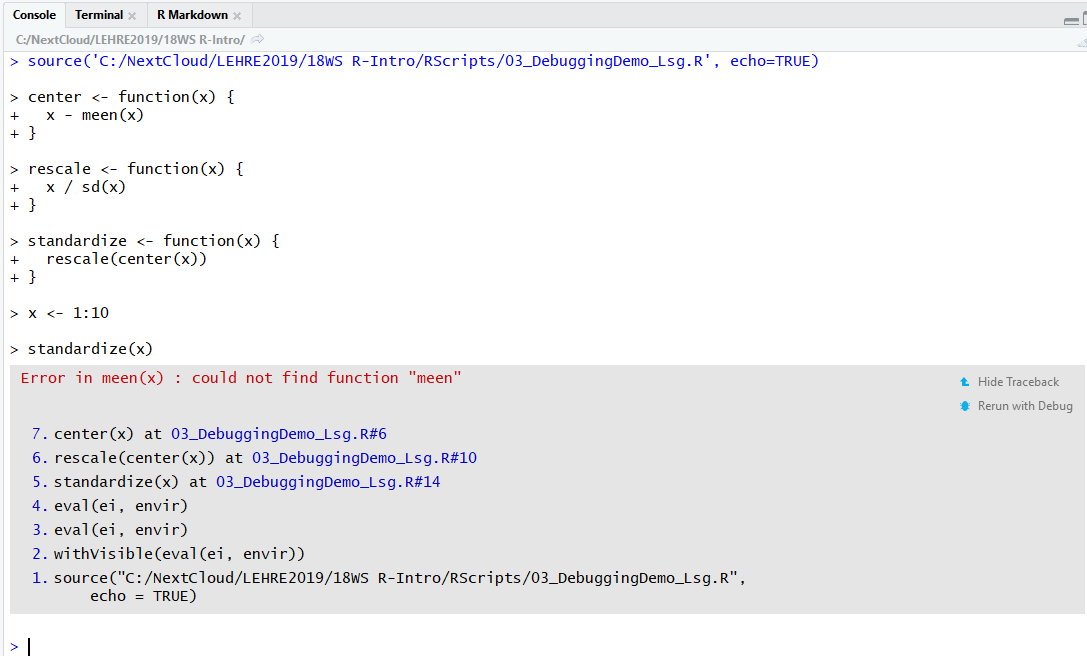
\includegraphics[width=0.60000\textwidth]{Images/03_Traceback.PNG}
\caption{\textbf{Abbildung 17}:
\href{https://google.github.io/styleguide/Rguide.xml\#comments}{Traceback
in RStudio}}
\end{figure}

\subsection*{Kommentare}\label{kommentare}
\addcontentsline{toc}{subsection}{Kommentare}

Ein gutes, nachvollziehbares und wiederverwendbares R-Programm basiert
nicht alleine auf einer effiziente Programmierung, sondern auch auf
einer entsprechende Beschreibung des Programms, bzw. bestimmten Teilen
des Programmcodes. Um ein Programm zu dokumentieren gelten folgende
Regeln:

\begin{itemize}
\tightlist
\item
  Kommentare beginnen mit \(\#\).
\item
  Kommentare enden mit dem Ende der Zeile.
\item
  Kommentare können am:

  \begin{itemize}
  \tightlist
  \item
    Anfang einer Zeile stehen: \(\#\) Erstellungsdatum: 12.11.2018
  \item
    Nach einem Codeteil: \emph{mean(x)} \(\#\) Berechnung des
    Mittelwertes von \emph{x}
  \end{itemize}
\item
  Sehr lange Kommentare in einer Zeile können durch
  \textit{Ctrl Shift /} der Bildschirmbreite angepasst werden.
\end{itemize}

Einige Richtlinien für Kommentare in R findet ihr unter
\href{https://google.github.io/styleguide/Rguide.xml\#comments}{Commenting
guidelines}

\section{Environment-Pane}\label{environment-pane}

Im R-Arbeitsbereich (\emph{environment}) besteht aus allen
Datenobjekten, die während einer R-Sitzung erstellt oder geladen werden.
Das Environment ist sozusagen das Arbeitsgedächtnis von R.

Beim Beenden von R wird man aufgefordert, den Arbeitsbereich zu
speichern. Wählt man Ja, speichert R eine Datei mit dem Namen
\emph{.RData} in das aktuelle Arbeitsverzeichnis.

Beim erneuten öffnen von R wird diese gespeicherte .RData wieder
geladen. Dadurch sind alle Datenobjekte der letzten Sitzung in R wieder
verfügbar. Auch auf alle in der letzten Sitzung eingegebenen Befehle
können mit den Aufwärts- und Abwärtspfeiltasten (\(\uparrow\),
\(\downarrow\)) der Tastatur zugegriffen werden.

Speichern, laden, oder löschen des Arbeitsbereich kann auch jederzeit
während einer R-Sitzung über das Menü, oder durch die entsprechenden
Schaltflächen im Environment-Pane durchführt werden. Das Löschen
bestimmter Objekte, bzw. des gesamten Environments ist auch von der
Konsole, bzw. vom Skript durch folgende Funktionen möglich:

\begin{Shaded}
\begin{Highlighting}[]
\NormalTok{  a       <-}\StringTok{ }\DecValTok{1}\OperatorTok{:}\DecValTok{100}
\NormalTok{  b       <-}\StringTok{ }\KeywordTok{c}\NormalTok{(}\StringTok{"Salzburg"}\NormalTok{, }\StringTok{"Wien"}\NormalTok{, }\StringTok{"Linz"}\NormalTok{)}
\NormalTok{  Seminar <-}\StringTok{ "R-Intro"}
\NormalTok{  V1      <-}\StringTok{ }\DecValTok{1}\OperatorTok{:}\DecValTok{10}
\NormalTok{  M1      <-}\StringTok{ }\KeywordTok{matrix}\NormalTok{(}\DecValTok{1}\NormalTok{, }\DecValTok{3}\NormalTok{, }\DecValTok{3}\NormalTok{)}
\NormalTok{  M2      <-}\StringTok{ }\KeywordTok{matrix}\NormalTok{(}\DecValTok{5}\NormalTok{, }\DecValTok{8}\NormalTok{, }\DecValTok{3}\NormalTok{)}
\NormalTok{  center  <-}\StringTok{ }\ControlFlowTok{function}\NormalTok{(x) \{}\KeywordTok{mean}\NormalTok{(x) }\OperatorTok{-}\StringTok{ }\KeywordTok{sd}\NormalTok{(x)\}}
  
  \KeywordTok{rm}\NormalTok{(a)           }\CommentTok{# löscht die Variable a}
  \KeywordTok{rm}\NormalTok{(V1, M1)      }\CommentTok{# löscht die Variablen V1 und M1}
  \KeywordTok{rm}\NormalTok{(}\DataTypeTok{list =} \KeywordTok{ls}\NormalTok{()) }\CommentTok{# löscht den gesamten Inhalt des Globalen Environments}
\end{Highlighting}
\end{Shaded}

Am rechten Rand der Symbolleiste kann man noch die Ansicht der Objekte
wählen:

\begin{itemize}
\tightlist
\item
  List: gibt nur die Namen der aktiven Objekte an.
\item
  Grid: zeigt neben dem Namen auch den Variablentyp (Type), die Länge
  der Variablen (Length), die Größer (Size) und die ersten paar Werte im
  jeweiligen Objekts. \emph{Grid ist die zu bevorzugende
  Darstellungsform des Environments}.
\end{itemize}

\begin{figure}
\centering
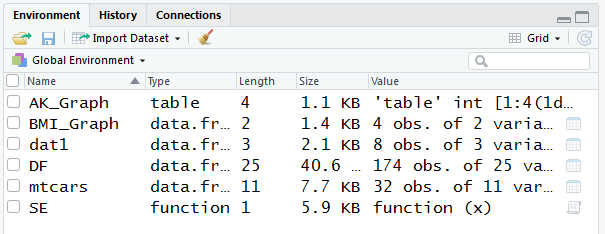
\includegraphics[width=0.50000\textwidth]{Images/04_Environment.PNG}
\caption{\textbf{Abbildung 18}: Das Arbeitsgedächtnis von RStudio}
\end{figure}

Bemerkenswert ist noch das Symbol Global Environment. Neben dem Global
Environment gibt es für jedes der geladenen Pakete einen eigenen
Arbeitsbereich, in welchem folgende Daten abgespeichert sind:

\begin{itemize}
\tightlist
\item
  die Funktionen des jeweiligen Paketes, sowie
\item
  Datensätze die zur Testung der jeweiligen Funktion verwendet werden
  können
\end{itemize}

\subsection*{History}\label{history}
\addcontentsline{toc}{subsection}{History}

Die R-Verlaufsdatei (History) ist eine Kopie aller Tastenanschläge
während einer Sitzung. Ein Rückgriff auf diese Verlaufsdatei kann vor
allem dann nützlich sein, wenn nicht alle Schritte in einer
R-Skriptdatei dokumentiert wurden. Die Rhistory-Datei ist eine einfache
Textdatei, in der alle Befehle, aber nicht die Ergebnisse aufgezeichnet
werden.

\begin{figure}
\centering
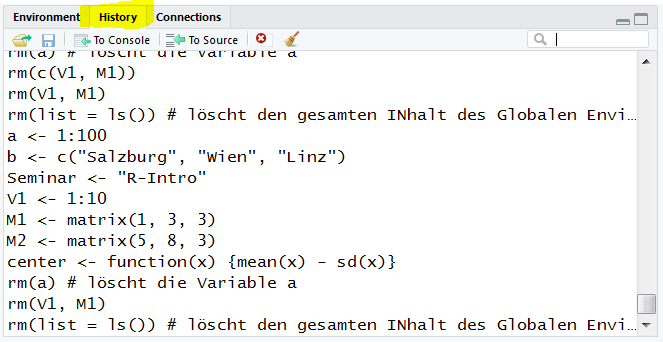
\includegraphics[width=0.50000\textwidth]{Images/04_History.PNG}
\caption{\textbf{Abbildung 19}: Die Historie von verwendeten Befehlen}
\end{figure}

Beachte die Symbole in dieser Ansicht. Man kann über diese:

\begin{itemize}
\tightlist
\item
  eine gespeicherte Historie von Befehlen laden.
\item
  die aktuelle Historie speichern.
\item
  Markierte Zeilen oder Blöcke der Historie an die Konsole senden und
  ausführen lassen (\emph{To Console}).
\item
  Markierte Zeilen oder Blöcke der Historie an die Source - also in ein
  geöffnetes R-Script - senden (\emph{To Source}).
\item
  markierte Einträge der Historie löschen.
\item
  die gesamte Historie löschen.
\end{itemize}

\subsection*{Connections}\label{connections}
\addcontentsline{toc}{subsection}{Connections}

Im RStudio-Verbindungsbereich (Connections) können Verbindung zu einer
Vielzahl von Datenquellen hergestellt werden\footnote{es ist jedoch kein
  Verbindungsmanager, wie z.B. PGAdmin, Toad oder SSMS.}. Vorwiegend
verwendet wird es für die Anbindung diverser Datenbanken. Ohne
Installation von Zusatzpaketen sind derzeit folgenden
Datenbankverbindungen\footnote{\href{https://de.wikipedia.org/wiki/Open_Database_Connectivity}{ODBC},
  \href{https://de.wikipedia.org/wiki/Apache_Spark}{Spark}} möglich:

\begin{figure}
\centering
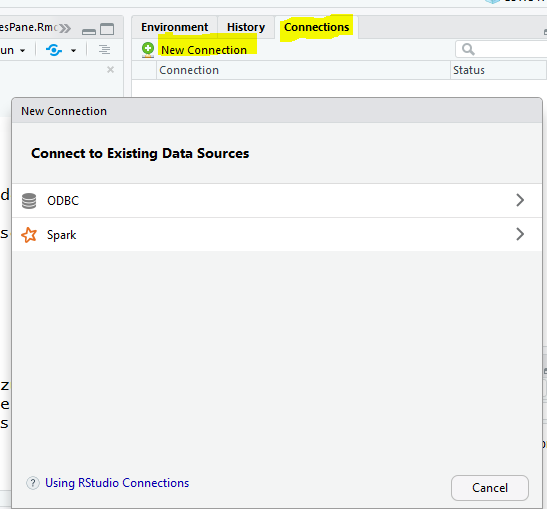
\includegraphics[width=0.50000\textwidth]{Images/04_Connections.PNG}
\caption{\textbf{Abbildung 20}: Datenbankverbindungen über Connections}
\end{figure}

\section{Files-Pane}\label{files-pane}

Über das Files-Pane können 5 unterschiedliche Registerkarte angesprochen
werden:

\begin{itemize}
\tightlist
\item
  Files
\item
  Plots
\item
  Packages
\item
  Help
\item
  Viewer
\end{itemize}

\subsection*{Files}\label{files}
\addcontentsline{toc}{subsection}{Files}

Entspricht im Wesentlichen einem Dateimanager. Angezeigt werden die
Inhalte des aktuellen Arbeitsverzeichnis, welches direkt unter den
Symbolen angezeigt wird. Man kann das Arbeitsverzeichnis auch in der
Konsole mit der Funktion \emph{getwd()} abfragen und gegebenenfalls auch
in eine Variable zur weitern Verwendung in einer Variablen speichern
(siehe nachfolgende Beispiele).

\begin{Shaded}
\begin{Highlighting}[]
\KeywordTok{getwd}\NormalTok{()       }\CommentTok{# gibt das aktuelle Arbeitsverzeichnis in der Konsole aus}
\NormalTok{WD <-}\StringTok{ }\KeywordTok{getwd}\NormalTok{() }\CommentTok{# speichert das Arbeitsverzeichnis in der Variablen WD}
\KeywordTok{setwd}\NormalTok{(}\StringTok{"E:/OwnCloud/LEHRE2019/18WS R-Intro"}\NormalTok{)}
\KeywordTok{setwd}\NormalTok{(WD)     }\CommentTok{# setzt das Arbeitsverzeichnis entsprechend des Inhaltes }
              \CommentTok{# der Variable WD}
\end{Highlighting}
\end{Shaded}

\subsection*{Plots}\label{plots}
\addcontentsline{toc}{subsection}{Plots}

Standardmäßig werden alle in R-erzeugten Plots in dieses Fenster
geschrieben. über die Symbolleiste ist es möglich, zwischen den bereits
generierten Plots zu blättern (\(\leftarrow\), \(\rightarrow\)), einen
Plot in einem eigenen Fenster zu öffnen (Zoom), die Graphiken zu
exportieren (als PDF oder als Bild in den verschiedensten Formaten, wie
z.B. png, jpg, eps, tiff, etc.), einzelne Graphen, bzw. alle Graphen zu
löschen.

\begin{figure}
\centering
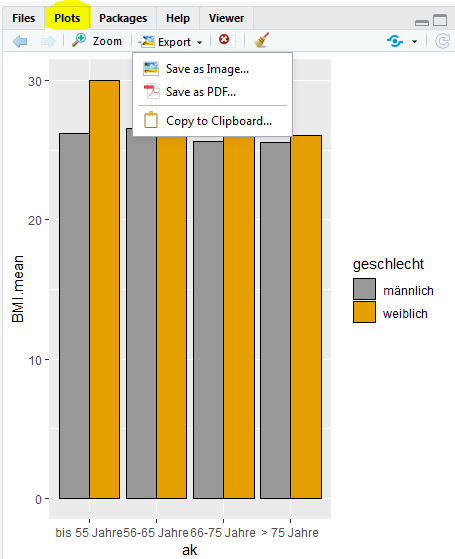
\includegraphics[width=0.30000\textwidth]{Images/05_Plots.PNG}
\caption{\textbf{Abbildung 21}: Das Ausgabefenster für Graphiken und
Bilder}
\end{figure}

\subsection*{Packages}\label{packages}
\addcontentsline{toc}{subsection}{Packages}

Eine zentrale Rolle bei der Verwendung von R spielen die Pakete. Im
diesem Fenster kann man einerseits die bereits geladenen Pakete sehen,
bzw. einen Update durchführen. Mit \emph{Packrat} steuert man bei
Projektarbeiten eine einheitliche Verwendung von Paketversionen für
allen beteiligten Projektmitarbeitern.

\begin{figure}
\centering
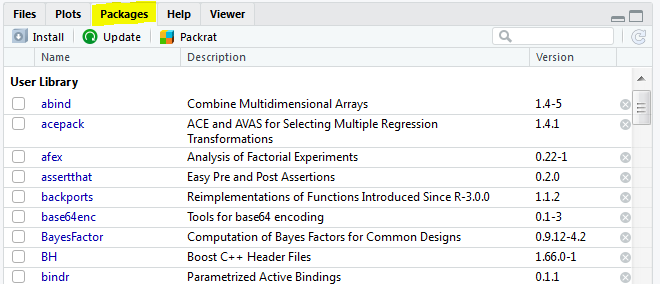
\includegraphics[width=0.50000\textwidth]{Images/05_Packages_Tab.PNG}
\caption{\textbf{Abbildung 22}: Pakete - der Motor von R}
\end{figure}

\subsubsection*{Umgang mit Paketen}\label{umgang-mit-paketen}
\addcontentsline{toc}{subsubsection}{Umgang mit Paketen}

Pakete sind Sammlungen zusätzlicher Funktionen, die bei Bedarf geladen
werden können. Sie enthalten häufig Beispieldaten, die zur Demonstration
dieser Funktionen verwendet werden können. Obwohl R in der Basisversion
schon mit einigen gängigen statistischen Funktionen und Modellen
ausgestattet ist, erfordern die meisten unserer Arbeiten zusätzliche
Pakete.

\subsubsection*{Installation und Verwendung von
Paketen}\label{installation-und-verwendung-von-paketen}
\addcontentsline{toc}{subsubsection}{Installation und Verwendung von
Paketen}

Um ein Paket verwenden zu können, muss es zuerst installiert und dann
geladen. Diese Schritte können in der Befehlszeile oder auf der
Registerkarte ``Pakete'' ausgeführt werden.

Im Fenster ``Pakete'' sieht man eine Liste aller derzeit auf Ihrem
Computer installierten Pakete sowie 2 Schaltflächen mit der Bezeichnung
``Install'' oder ``Update''. Um ein neues Paket zu installieren, klickt
man einfach auf die Schaltfläche \emph{Install}.

Für die Arbeit mit Pakten ist folgendes zu beachten:

\begin{itemize}
\tightlist
\item
  R-Pakete müssen nur einmal installiert werden (bis R aktualisiert oder
  neu installiert wird).
\end{itemize}

\begin{figure}
\centering
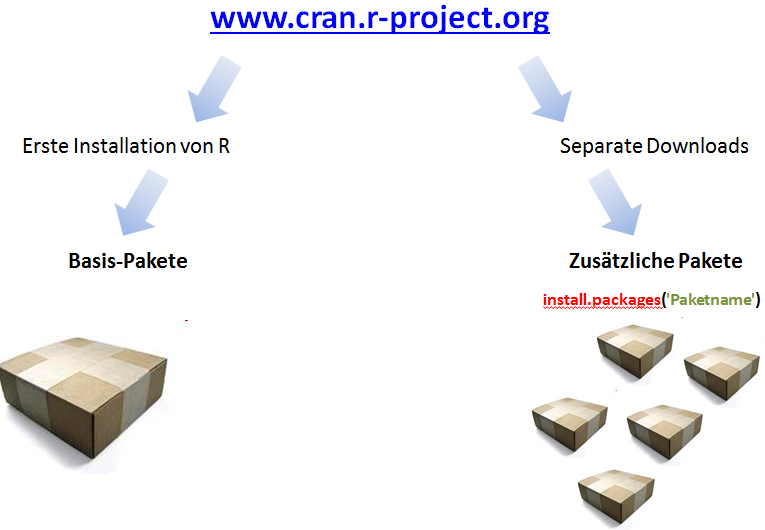
\includegraphics[width=0.40000\textwidth]{Images/05_Package_Libraries.PNG}
\caption{\textbf{Abbildung 23}: Laden von Paketen}
\end{figure}

\begin{itemize}
\tightlist
\item
  Bei jedem Start einer neuen R-Sitzung muss jedoch jedes Paket, dass in
  der aktuellen Sitzung verwendet werden soll, geladen werden.
\end{itemize}

\begin{figure}
\centering
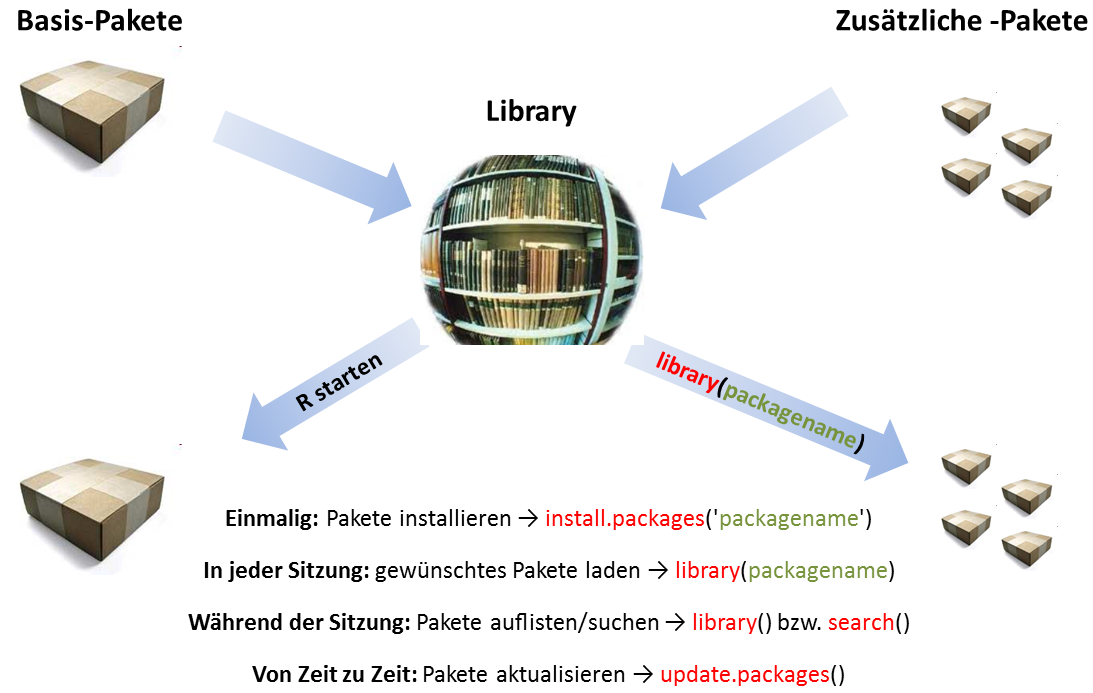
\includegraphics[width=0.40000\textwidth]{Images/05_Package_Verwendung.PNG}
\caption{\textbf{Abbildung 24}: Verwenden von Paketen}
\end{figure}

In der Abbildung sind auch die Funktionen zum Installieren und
Aktualisieren angegeben. Da bei vielen Paketen fortlaufend
Änderungen/Erweiterungen und Verbesserungen vorgenommen werden, ist in
regelmäßigen Abständen nach Updates der geladenen Pakete zu suchen. Dies
ist am einfachsten über das Menü \emph{Tools} \(\rightarrow\)
\emph{Check for Package Updates}, bzw. über die Funktion
\emph{update\_packages()} (ist im Package \emph{utils} enthalten) in der
Konsole oder über den Editor durchzuführen.

\subsection*{Help}\label{help}
\addcontentsline{toc}{subsection}{Help}

Verschiedenen Möglichkeiten in R Hilfe in Anspruch zu nehmen, haben wir
ja bereits in vorangegangenen Kapiteln angesprochen. Die unter dieser
Registrierkarte befindliche Hilfe zu den einzelnen Funktionen ist in
technischer Sicht sehr aufschlussreich, da es einer vollständigen
Dokumentation der Funktionen innerhalb von Paketen entspricht.

Für Einsteiger in R kann diese Hilfe jedoch auch schnell \emph{zu
technisch} werden. Daher empfiehlt es sich, bei Bedarf auf die bereits
hingewiesenen Alternativen von benutzerfreundlicheren Websites
zurückzugreifen.

\subsection*{Viewer}\label{viewer}
\addcontentsline{toc}{subsection}{Viewer}

RStudio enthält einen Viewer-Bereich, in dem lokaler Webinhalt angezeigt
werden kann. Beispielsweise Webgrafiken, die mit Paketen wie googleVis,
htmlwidgets und rCharts generiert wurden, oder lokale Webanwendung, die
mit Shiny, Rook oder OpenCPU erstellt wurde.

Zu beachten ist, dass der Viewer-Bereich nur für lokale Webinhalte
verwendet werden kann. Bei den Inhalten kann es sich entweder um
statische HTML-Dateien handeln, oder um eine lokal ausgeführte
Webanwendung handeln.

Für die aktuelle Lehrveranstaltung wird dieses Fenster keine, bzw. nur
eine nachrangige Rolle spielen, daher verzichten wir fürs Erste auf
weitere Ausführungen zu diesen Themen.

\section{Rlernen}\label{rlernen}

\subsection*{Top-Down vs.~Bottom-Up}\label{top-down-vs.bottom-up}
\addcontentsline{toc}{subsection}{Top-Down vs.~Bottom-Up}

Wie beim Erlernen einer neuen Sprache, gibt es auch für
Programmiersprachen verschiedene Ansätze. Im Bottom-Up Ansatz wird man
sich zuerst mit den Elementen einer Sprache (Vokabeln) und deren
korrekter Zusammensetzung (Grammatik) beschäftigen. Dieser Ansatz ist
vor allem zu Beginn oft schwierig und mühsam, da die Zusammenhänge erst
nach einiger Zeit klar werden und die (erfolgreiche) Anwendung der
Sprache erst nach einer mehr oder weniger langen \emph{Vorlaufzeit}
möglich ist.

Beim Top-Down Ansatz wird man direkt mit dem gesamten Umfang der Sprache
konfrontiert. Sprachbausteine werden von anderen übernommen, Details zur
Struktur, den Regeln und eine Erweiterung des Wortschatzes bilden sich
durch die Übernahme von Experten.

Bei der Erlernung einer Programmiersprache bietet sich vor allem durch
die unzähligen Möglichkeiten von Beispielen und Vorlagen im Internet,
sowie die bis ins letzte Detail ausgearbeiteten Hilfeseiten zu den
jeweiligen Sprachen eine Mischung des Lernvorganges an. Wir werden den
Einstieg in die Programmiersprache R mit einem Top-Down Ansatz beginnen.

\subsubsection*{Top Down - Copy und
Paste}\label{top-down---copy-und-paste}
\addcontentsline{toc}{subsubsection}{Top Down - Copy und Paste}

Erstelle eine neue R-Script-Datei. Kopiere den nachfolgenden Code in
diese neue Datei und speicher diesen unter den Namen
\emph{06\_R\_Paste\_Copy\_Intro.R} in ein Verzeichnis deiner Wahl.

\begin{Shaded}
\begin{Highlighting}[]
\CommentTok{#------------------------------- Initialisierung}
\KeywordTok{rm}\NormalTok{(}\DataTypeTok{list =} \KeywordTok{ls}\NormalTok{())}
\ControlFlowTok{if}\NormalTok{ (}\OperatorTok{!}\KeywordTok{require}\NormalTok{(}\StringTok{"pacman"}\NormalTok{)) }\KeywordTok{install.packages}\NormalTok{(}\StringTok{"pacman"}\NormalTok{)}
\NormalTok{pacman}\OperatorTok{::}\KeywordTok{p_load}\NormalTok{(ggplot2)}
\CommentTok{#------------------------------- Ende Initialisierung}
\end{Highlighting}
\end{Shaded}

Öffne einen Browser (Mozilla, IE, Chrome, \ldots{}) und bearbeite
folgende Aufgabenstellungen:

\subsubsection*{Copy und Paste
(Aufgabenblock)}\label{copy-und-paste-aufgabenblock}
\addcontentsline{toc}{subsubsection}{Copy und Paste (Aufgabenblock)}

\begin{enumerate}
\def\labelenumi{\arabic{enumi}.}
\tightlist
\item
  Kopiere von
  \href{http://www.cookbook-r.com/Basics/Indexing_into_a_data_structure/}{Indexing
  with numbers and names} die Zeile \(v <- c(1,4,4,3,2,2,3)\) in das
  neue Skript und führe diese Zeile aus. Beschreibe die Auswirkung
  dieser Zeile bezüglich der Änderungen im Konsolen- und
  Environment-Fenster.
\item
  Kopiere (aus der Website) die Zeile \(v[c(2,3,4)]\) in das neue Skript
  und führe diese Zeile aus. Beschreibe die Auswirkung dieser Zeile
  bezüglich der Änderungen im Konsolen- und Environment-Fenster.
\item
  Gehe zur folgenden Website:
  \href{http://www.cookbook-r.com/Graphs/Bar_and_line_graphs_(ggplot2)/}{Bar
  and line graphs (ggplot2)} und kopiere aus dem Block \emph{Bar graphs
  of values} die ersten vier Zeilen in den Editor. Führe diese Zeilen
  aus und diskutiere das Ergebnis.
\item
  Kopiere nun von dieser Website den zweiten Codeblock und führe den
  Code aus. Diskutiere das Ergebnis (siehe Plots-Fenster).
\item
  Kopiere nun die zwei Codeblocks im Kapitel ``Bar graphs of counts''
  und führe den Code aus. Beachte vor allem, woher die Daten (tips)
  kommen!
\item
  Gebe die Befehle data() und ?tips, bzw. ?french\_fries ein und
  diskutiere das Ergebnis.
\item
  Führe folgende zwei Zeilen aus:

  \begin{itemize}
  \tightlist
  \item
    Dat\_FF \textless{}- french\_fries
  \item
    str(Dat\_FF)
  \end{itemize}
\item
  Laden mit Hilfe von Import Dataset die SPSS-Datei ``bigfive.sav'' und
  kopiere die entsprechenden Befehle in dein Skript.
\item
  Lade nun die Datei ``bigfive\_excel.xlsx'' (ebenfalls in ../Data/) mit
  Hilfe von Import Dataset und kopiere die entsprechenden R-Befehle in
  den Editor.
\end{enumerate}

\subsection*{Objekte in R (bottom up)}\label{objekte-in-r-bottom-up}
\addcontentsline{toc}{subsection}{Objekte in R (bottom up)}

In R kann alles als Objekt gespeichert werden.

\begin{itemize}
\tightlist
\item
  Einzelne Werte Mehrere Werte (z. B. als Datensatz mit Rohdaten)
\item
  Tabellen
\item
  Statistische Modelle
\item
  Ergebnisse statistischer Analysen
\item
  Funktionen, etc.
\end{itemize}

Alle Objekte, die in einer R-Sitzung erstellt oder geöffnet wurden,
liegen im sogenannten Environment (Arbeitsbereich). Bei der letzten
Übungsaufgabe wurden folgende Objekte im Environment angelegt:

\begin{figure}
\centering
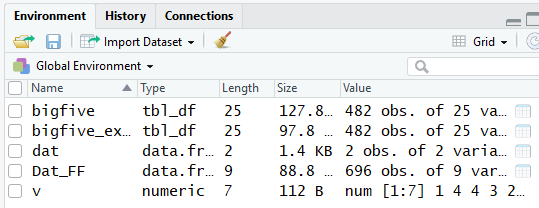
\includegraphics[width=0.50000\textwidth]{Images/06_Environment.PNG}
\caption{\textbf{Abbildung 25}: Environment der letzten Übungsaufgabe}
\end{figure}

Das Anlegen eines Objektes im Environment erfolgt über die Zuweisung
\emph{Objektname \textless{}- Objektinhalt}. Die Zuweisung über das
\emph{\textless{}-} ist dabei R-spezifisch. Man kann auch das übliche
\emph{=} verwenden, wobei dieses in R auch noch eine andere Eigenschaft
hat (Details später).

Für die Vergabe von \emph{Objektnamen} sind folgende Regeln zu beachten:

\begin{itemize}
\tightlist
\item
  Objektname darf nicht mit Zahl beginnen
\item
  Objektname darf keine Operatoren enthalten (+, -, * etc.)
\item
  Auf Groß- und Kleinschreibung achten
\end{itemize}

In gibt es eine Vielzahl von verschiedenen Objekttypen. Die
grundlegenden Objekttypen (und deren Gemeinsamkeit mit SPSS-Datentypen)
sind:

\begin{itemize}
\tightlist
\item
  Vektoren \(\rightarrow\) ordinale/metrische Variablen

  \begin{itemize}
  \tightlist
  \item
    numeric (Zahlen)
  \item
    character (Buchstaben)
  \end{itemize}
\item
  Faktoren \(\rightarrow\) nominale/ordinale Variablen

  \begin{itemize}
  \tightlist
  \item
    nominale Variable
  \item
    Kategorien des Faktors = levels (kann Buchstaben oder Zahlen
    enthalten)
  \end{itemize}
\item
  Data Frames (mehrere Zeilen und Spalten) \(\rightarrow\) Datensatz

  \begin{itemize}
  \tightlist
  \item
    Spalten (Vektoren und Faktoren
  \item
    Zeilen (Fälle, z. B. Versuchspersonen)
  \end{itemize}
\item
  Matrizen \(\rightarrow\) in SPSS nicht vorhanden

  \begin{itemize}
  \tightlist
  \item
    viele Zeilen und Spalten
  \item
    es können nur Daten eines Typs (z. B. numerische Werte, oder nur
    Faktoren, etc.) dargestellt werden.
  \end{itemize}
\item
  Arrays \(\rightarrow\) in SPSS nicht vorhanden

  \begin{itemize}
  \tightlist
  \item
    Kombination mehrerer Matrizen (Zusammenfassungen von Elementen des
    gleichen Datentyps (numeric, character, logical), werden über 2 oder
    mehr Indizes adressiert).
  \end{itemize}
\item
  Listen \(\rightarrow\) in SPSS nicht vorhanden

  \begin{itemize}
  \tightlist
  \item
    Kombination mehrerer Objekte
  \item
    Listen können beliebige Objekte enthalten, auch Objekte
    verschiedenen Typs.
  \item
    Im Unterschied zu Data Frames und Arrays können auch Objekte
    unterschiedlicher Länge gespeichert werden.
  \end{itemize}
\end{itemize}

\subsubsection*{Vektoren}\label{vektoren}
\addcontentsline{toc}{subsubsection}{Vektoren}

Das einfachste Objekt ist ein Vektor, der aus mehreren Elementen
besteht. Öffne eine neue Skript-Datei und kopiere folgenden Inhalte in
diese Datei:

\begin{Shaded}
\begin{Highlighting}[]
\NormalTok{  name       <-}\StringTok{ "Max Mustermann"} \CommentTok{# Beachte das Fenster Environment}
\NormalTok{  mein.alter <-}\StringTok{ }\DecValTok{35}
\NormalTok{  mein.alter}
\NormalTok{  mein.alter }\OperatorTok{+}\StringTok{ }\DecValTok{10}
\NormalTok{  mein.alter.}\DecValTok{1}\NormalTok{ <-}\StringTok{ }\NormalTok{mein.alter }\OperatorTok{+}\StringTok{ }\DecValTok{10}
\NormalTok{  mein.alter.}\DecValTok{1}
\end{Highlighting}
\end{Shaded}

Speichere die Datei unter dem Namen \emph{06\_Objekte.R}. Führe nun die
Inhalte zeilenweise aus und diskutiere die Wirkung der einzelnen Zeilen!
Kopiere nun den folgenden Code in die Datei und führe diesen Code
zeilenweise aus. Was passiert dabei im Environment?

\begin{Shaded}
\begin{Highlighting}[]
  \CommentTok{# Fasse Zahlen in einem Vektor zusammen}
\NormalTok{    alter    <-}\StringTok{ }\KeywordTok{c}\NormalTok{(}\DecValTok{19}\NormalTok{, }\DecValTok{24}\NormalTok{, }\DecValTok{20}\NormalTok{, }\DecValTok{19}\NormalTok{) }\CommentTok{# Beispiel: Alter von 4 Studenten}
\NormalTok{    kurs.num <-}\StringTok{ }\KeywordTok{c}\NormalTok{(}\DecValTok{1}\NormalTok{, }\DecValTok{3}\NormalTok{, }\DecValTok{2}\NormalTok{, }\DecValTok{2}\NormalTok{) }\CommentTok{# Beispiel: Zugeh?rigkeit zu einem von 3 Kursen}
  \CommentTok{# Fasse Buchstaben in einem Vektor zusammen}
\NormalTok{    kurs.bez <-}\StringTok{ }\KeywordTok{c}\NormalTok{(}\StringTok{'Kurs1'}\NormalTok{, }\StringTok{'Kurs3'}\NormalTok{, }\StringTok{'Kurs2'}\NormalTok{, }\StringTok{'Kurs2'}\NormalTok{)}
  \CommentTok{# Zeige Inhalt des Vektors}
\NormalTok{    alter}
\NormalTok{    kurs.num}
\NormalTok{    kurs.bez}
\end{Highlighting}
\end{Shaded}

Um auf einzelne Elemente eines Vektors zuzugreifen gibt es mehrere
Möglichkeiten.

\begin{enumerate}
\def\labelenumi{\arabic{enumi}.}
\tightlist
\item
  Zugriff durch direkte Indizierung
\item
  Zugriff durch Variablen (Vektoren), in denen die Indizes der Elemente
  auf die man zugreifen will abgespeichert sind.
\end{enumerate}

Der folgende Code zeigt beide dieser Möglichkeiten. Kopiere den Code in
das Skript und führe diesen zeilenweise aus.

\begin{Shaded}
\begin{Highlighting}[]
\NormalTok{    alter[}\DecValTok{2}\NormalTok{]   }\CommentTok{# direkte Indizierung, das zweite Element des Vektors wird ausgegeben}
\NormalTok{    alter[}\DecValTok{1}\OperatorTok{:}\DecValTok{3}\NormalTok{] }\CommentTok{# direkte Indizierung, das erste bis dritte Element des Vektors wird ausgegeben.}
               \CommentTok{# Beachte dabei die Verwendung von :}
    \DecValTok{2}\OperatorTok{:}\DecValTok{4}        \CommentTok{# erzeugen eines Vektors der in ganzen Schritten von 2 beginnend bis 4 hinaufz?hlt}
\NormalTok{    v_}\DecValTok{1}\NormalTok{ <-}\StringTok{ }\DecValTok{2}\OperatorTok{:}\DecValTok{4} \CommentTok{# speichern des Vektors in der Variablen v_1}
\NormalTok{    alter[v_}\DecValTok{1}\NormalTok{] }\CommentTok{# Verwendung des Vektors v_ind um die Elemente des Vektors alter auszugeben}
\NormalTok{    v_}\DecValTok{2}\NormalTok{ <-}\StringTok{ }\KeywordTok{seq}\NormalTok{(}\DataTypeTok{from =} \DecValTok{1}\NormalTok{,  }\CommentTok{# erzeugen einer Sequenz von Zahlen, die mit 1 beginnt, bei 4 endet}
               \DataTypeTok{to   =} \DecValTok{4}\NormalTok{,  }\CommentTok{# und in 2-er Schritten hinaufz?hlt}
               \DataTypeTok{by   =} \DecValTok{2}\NormalTok{)  }\CommentTok{# Die Sequenz wird in v_2 gespeichert.}
\NormalTok{    alter[v_}\DecValTok{2}\NormalTok{] }\CommentTok{# Verwendung des Vektors v_2 um die Elemente des Vektors alter auszugeben.}
\NormalTok{    alter[}\OperatorTok{-}\DecValTok{4}\NormalTok{]  }\CommentTok{# um Werte eines Vektors nicht anzuzeigen, kann der Index des entsprechenden}
               \CommentTok{# Wertes mit einem f?hrenden Minuszeichen angegeben werden. Dadurch wird der }
               \CommentTok{# vierte Eintrag des Vektors nicht ausgegeben!}
\NormalTok{    v_}\DecValTok{3}\NormalTok{  <-}\StringTok{ }\KeywordTok{c}\NormalTok{(}\DecValTok{1}\NormalTok{, }\DecValTok{3}\NormalTok{, }\DecValTok{4}\NormalTok{) }\CommentTok{# auch die Verwendung der Funktion c() kann zur Erstellung von Indexlisten}
                       \CommentTok{# verwendet werden.}
\NormalTok{    alter[v_}\DecValTok{3}\NormalTok{]}
\end{Highlighting}
\end{Shaded}

Um festzustellen, um welche Art von Daten, bzw. welche Klasse von Daten
(numerisch, alphanumerisch, Datum, etc.) im jeweiligen Objekt
abgespeichert sind, kann die Funktion \emph{class()} verwendet werden.
Das Ändern des Datentyps eines (einfachen) Objektes ist durch die
Funktionen \emph{as.numeric(variable)}, bzw.
\emph{as.character(variable)} möglich. Darüber hinaus gibt es noch viele
Funktionen, die bezüglich des Datentyps von Objekten verwendet werden
können. Einige dieser Funktionen werden bei den entsprechenden
Anwendungen im Detail besprochen.

\begin{Shaded}
\begin{Highlighting}[]
    \KeywordTok{class}\NormalTok{(alter) }\CommentTok{# Zeigt an, zu welcher Klasse die Inhalte des Objekts alter geh?ren}
\NormalTok{    alter_char <-}\StringTok{ }\KeywordTok{as.character}\NormalTok{(alter) }\CommentTok{# wandelt num in char}
    \KeywordTok{class}\NormalTok{(alter_char)}
\NormalTok{    alter_num  <-}\StringTok{ }\KeywordTok{as.numeric}\NormalTok{(alter_char) }\CommentTok{# wandelt char in num}
    \KeywordTok{class}\NormalTok{(alter_num)}
\end{Highlighting}
\end{Shaded}

Das Wandeln von numerisch auf alphanumerisch und vice versa sind jedoch
häufig gebrauchte Funktionen, vor allem bei der Übernahme von Daten aus
anderen Anwendungen.

\subsubsection*{Arithmetische Operator
(Vektorenrechnung)}\label{arithmetische-operator-vektorenrechnung}
\addcontentsline{toc}{subsubsection}{Arithmetische Operator
(Vektorenrechnung)}

In R werden + - * / für Addition, Subtraktion, Multiplikation und
Division verwendet. Diese Operatoren werden auf alle Elemente eines
Vektors angewendet:

\begin{Shaded}
\begin{Highlighting}[]
\NormalTok{    Geburtsjahr <-}\StringTok{ }\DecValTok{2018} \OperatorTok{-}\StringTok{ }\NormalTok{alter}
\NormalTok{    Alter_Tage  <-}\StringTok{ }\NormalTok{alter }\OperatorTok{*}\StringTok{ }\DecValTok{365}
\NormalTok{    v1 <-}\StringTok{ }\DecValTok{1}\OperatorTok{:}\DecValTok{5}
\NormalTok{    v2 <-}\StringTok{ }\NormalTok{v1}\OperatorTok{*}\DecValTok{2}
\NormalTok{    v2}
\NormalTok{    v2 <-}\StringTok{ }\NormalTok{v2 }\OperatorTok{-}\StringTok{ }\NormalTok{.}\DecValTok{5}
\NormalTok{    v2}
\NormalTok{    v3 <-}\StringTok{ }\KeywordTok{c}\NormalTok{(}\DecValTok{2}\NormalTok{, }\DecValTok{5}\NormalTok{, }\DecValTok{8}\NormalTok{, }\DecValTok{10}\NormalTok{, }\DecValTok{12}\NormalTok{)}
\NormalTok{    v4 <-}\StringTok{ }\NormalTok{v1 }\OperatorTok{*}\StringTok{ }\NormalTok{v3}
\end{Highlighting}
\end{Shaded}

\subsubsection*{Weitere nützliche
Vektor-Funktionen}\label{weitere-nutzliche-vektor-funktionen}
\addcontentsline{toc}{subsubsection}{Weitere nützliche
Vektor-Funktionen}

Neben der bereits besprochenen Funktion \emph{seq()}, sind auch
nachfolgende Funktionen für das Arbeiten mit Vektoren oft nützlich. Da
wir diese Funktionen laufend verwenden, werden hier nicht alle
Einzelheiten diskutiert - verwende dazu die help() Funktion.

\begin{Shaded}
\begin{Highlighting}[]
\NormalTok{    y <-}\StringTok{ }\KeywordTok{c}\NormalTok{(}\StringTok{"a"}\NormalTok{, }\StringTok{"b"}\NormalTok{, }\StringTok{"c"}\NormalTok{, }\StringTok{"d"}\NormalTok{) }
    \KeywordTok{rep}\NormalTok{(y, }\DecValTok{3}\NormalTok{) }\CommentTok{# Replicate Elements of Vectors and Lists}
    \KeywordTok{rep}\NormalTok{(}\DecValTok{1}\OperatorTok{:}\DecValTok{5}\NormalTok{, }\DecValTok{4}\NormalTok{)}
\NormalTok{    n <-}\StringTok{ }\KeywordTok{c}\NormalTok{(}\DecValTok{2}\NormalTok{, }\DecValTok{4}\NormalTok{, }\DecValTok{1}\NormalTok{, }\DecValTok{10}\NormalTok{)}
    \KeywordTok{rep}\NormalTok{(y, n)}
\NormalTok{    y <-}\StringTok{ }\KeywordTok{c}\NormalTok{(}\StringTok{"i"}\NormalTok{, }\StringTok{"i"}\NormalTok{, }\StringTok{"a"}\NormalTok{, }\StringTok{"a"}\NormalTok{, }\StringTok{"E"}\NormalTok{, }\StringTok{"E"}\NormalTok{, }\StringTok{"E"}\NormalTok{, }\StringTok{"E"}\NormalTok{, }\StringTok{"U"}\NormalTok{)}
    \KeywordTok{unique}\NormalTok{(y) }\CommentTok{# eindeutige Elemente eines Vektors}
    \KeywordTok{table}\NormalTok{(y)  }\CommentTok{# erstellt eine Kreuztabelle}
    \KeywordTok{sort}\NormalTok{(y)   }\CommentTok{# sortieren von Vektoren (ACHTUNG: order() bei Datenstrukturen verwenden, siehe sp?ter)}
    \KeywordTok{paste}\NormalTok{(y, }\DecValTok{1}\OperatorTok{:}\DecValTok{9}\NormalTok{)}
    \KeywordTok{paste0}\NormalTok{(y, }\DecValTok{1}\OperatorTok{:}\DecValTok{9}\NormalTok{)}
\end{Highlighting}
\end{Shaded}

\subsubsection*{Logische Vektoren}\label{logische-vektoren}
\addcontentsline{toc}{subsubsection}{Logische Vektoren}

Ein logischer Vektor besteht aus TRUE und FALSE Elementen. Diese
Vektoren folgen einer sogenannten \emph{Boolean-Logik} mit diesen
Prinzipien (in R wird das logische UND mit \(\&\), das logische ODER mit
\(|\) geschrieben:

\begin{itemize}
\tightlist
\item
  T und T gleicht T (T \& T \(\rightarrow\) T)
\item
  F und F gleicht F (F \& F \(\rightarrow\) F)
\item
  T und F gleicht F (T \& F \(\rightarrow\) F)
\item
  T oder T gleicht T (T \textbar{} T \(\rightarrow\) T)
\item
  F oder F gleicht F (T \textbar{} T \(\rightarrow\) F)
\item
  T oder F gleicht T (T \textbar{} T \(\rightarrow\) T)
\end{itemize}

Werden Klammern verwendet gilt: Ausdruck innerhalb der Klammern wird
zuerst ausgewertet! Mit der \emph{sum()} Funktion können die Anzahl der
wahren (T) Elemente eine Vektors ermittelt werden. Ein
Anwendungsbeispiel wäre z.B., mit einer logischen Abfrage zu ermitteln,
wie viele Ja-Antworten in einem Vektor bestehend aus Ja/Nein Antworten
vorhanden sind (siehe nachfolgenden Code).

\begin{Shaded}
\begin{Highlighting}[]
\NormalTok{    T }\OperatorTok{&}\StringTok{ }\NormalTok{T}
\NormalTok{    F }\OperatorTok{&}\StringTok{ }\NormalTok{F}
\NormalTok{    T }\OperatorTok{&}\StringTok{ }\NormalTok{F}
\NormalTok{    T }\OperatorTok{|}\StringTok{ }\NormalTok{T}
\NormalTok{    F }\OperatorTok{|}\StringTok{ }\NormalTok{F}
\NormalTok{    T }\OperatorTok{|}\StringTok{ }\NormalTok{F}
\NormalTok{    (T }\OperatorTok{&}\StringTok{ }\NormalTok{F) }\OperatorTok{|}\StringTok{ }\NormalTok{T}
    
\NormalTok{    Vec <-}\StringTok{ }\KeywordTok{c}\NormalTok{(}\KeywordTok{rep}\NormalTok{( }\StringTok{"Nein"}\NormalTok{, }\DataTypeTok{len =} \DecValTok{25}\NormalTok{), }
                   \KeywordTok{rep}\NormalTok{( }\StringTok{"Ja"}\NormalTok{, }\DataTypeTok{len =} \DecValTok{43}\NormalTok{),}
                   \KeywordTok{rep}\NormalTok{( }\StringTok{"Weder noch"}\NormalTok{, }\DataTypeTok{len =} \DecValTok{12}\NormalTok{))}
    \KeywordTok{sum}\NormalTok{(Vec }\OperatorTok{==}\StringTok{ "Ja"}\NormalTok{)}
\end{Highlighting}
\end{Shaded}

\subsubsection*{Der \%in\% Operator und die
which()-Funktion}\label{der-in-operator-und-die-which-funktion}
\addcontentsline{toc}{subsubsection}{Der \%in\% Operator und die
which()-Funktion}

Der \%in\% Operator wird benutzt, um einem Vektor mehrere Elemente zu
entnehmen. Dies kann auch mit sämtlichen Teilfragen und dem \textbar{}
Operator durchgeführt werden. Nachfolgend erzeugen wir einen logischen
Vektor \emph{InVec}, der T ist, wenn \emph{Vec} ``Nein'' oder ``Weder
noch'' enthält:

\begin{Shaded}
\begin{Highlighting}[]
\NormalTok{    InVec <-}\StringTok{ }\NormalTok{Vec }\OperatorTok\StringTok{ }\KeywordTok{c}\NormalTok{(}\StringTok{"Nein"}\NormalTok{, }\StringTok{"Weder noch"}\NormalTok{)}
\NormalTok{    InVec}
\end{Highlighting}
\end{Shaded}

Logische Operatoren und die \emph{which()} Funktion bieten eine
effiziente Möglichkeit auf Elemente eines Vektors zuzugreifen. Betrachte
folgende Beispiele:

\begin{Shaded}
\begin{Highlighting}[]
\NormalTok{    VRand <-}\StringTok{ }\KeywordTok{rnorm}\NormalTok{(}\DecValTok{200}\NormalTok{, }\DataTypeTok{mean =} \DecValTok{50}\NormalTok{, }\DataTypeTok{sd =} \DecValTok{8}\NormalTok{)}
\NormalTok{    VRand_GT_Mean_Indices <-}\StringTok{ }\NormalTok{VRand }\OperatorTok{>=}\StringTok{ }\KeywordTok{mean}\NormalTok{(VRand, }\DataTypeTok{na.rm =}\NormalTok{ T)}
\NormalTok{    VRand[VRand_GT_Mean_Indices]}
    \KeywordTok{sum}\NormalTok{(VRand_GT_Mean_Indices)}
    \KeywordTok{sum}\NormalTok{(VRand_GT_Mean_Indices }\OperatorTok{==}\StringTok{ "TRUE"}\NormalTok{)}
    \KeywordTok{sum}\NormalTok{(VRand_GT_Mean_Indices }\OperatorTok{!=}\StringTok{ "TRUE"}\NormalTok{)}
    \KeywordTok{any}\NormalTok{(VRand_GT_Mean_Indices)}
    \KeywordTok{which}\NormalTok{(VRand_GT_Mean_Indices)}
    \KeywordTok{which}\NormalTok{(VRand_GT_Mean_Indices }\OperatorTok{==}\StringTok{ "TRUE"}\NormalTok{)    }
    \KeywordTok{which}\NormalTok{(VRand_GT_Mean_Indices }\OperatorTok{==}\StringTok{ "FALSE"}\NormalTok{)    }
\end{Highlighting}
\end{Shaded}

\subsubsection*{Aufgabenblock Vektoren}\label{aufgabenblock-vektoren}
\addcontentsline{toc}{subsubsection}{Aufgabenblock Vektoren}

Kopiere den folgenden Code in eine neues R-Skript und speichere dieses
unter dem Namen \emph{06\_Objekte\_Aufgaben}.

\begin{Shaded}
\begin{Highlighting}[]
    \CommentTok{# Vektoren - Combine}
\NormalTok{    id     <-}\StringTok{ }\KeywordTok{c}\NormalTok{(}\DecValTok{11}\NormalTok{, }\DecValTok{16}\NormalTok{, }\DecValTok{17}\NormalTok{, }\DecValTok{18}\NormalTok{, }\DecValTok{19}\NormalTok{, }\DecValTok{20}\NormalTok{, }\DecValTok{23}\NormalTok{) }\CommentTok{# c() entspr. combine; <- Zuweisung zu einer Variablen}
\NormalTok{    Geschlecht <-}\StringTok{ }\KeywordTok{c}\NormalTok{(}\StringTok{"m?nnlich"}\NormalTok{, }\StringTok{"weiblich"}\NormalTok{)}
\NormalTok{    sex    <-}\StringTok{ }\KeywordTok{c}\NormalTok{(}\DecValTok{1}\NormalTok{, }\DecValTok{1}\NormalTok{, }\DecValTok{7}\NormalTok{, }\DecValTok{1}\NormalTok{, }\DecValTok{1}\NormalTok{, }\DecValTok{2}\NormalTok{, }\DecValTok{2}\NormalTok{)}
\NormalTok{    lalt   <-}\StringTok{ }\KeywordTok{c}\NormalTok{(}\DecValTok{2}\NormalTok{, }\DecValTok{3}\NormalTok{, }\DecValTok{2}\NormalTok{, }\DecValTok{3}\NormalTok{, }\DecValTok{1}\NormalTok{, }\DecValTok{1}\NormalTok{, }\DecValTok{2}\NormalTok{)}
\NormalTok{    gross  <-}\StringTok{  }\KeywordTok{c}\NormalTok{(}\DecValTok{173}\NormalTok{, }\DecValTok{166}\NormalTok{, }\DecValTok{178}\NormalTok{, }\DecValTok{154}\NormalTok{, }\DecValTok{164}\NormalTok{, }\DecValTok{389}\NormalTok{, }\DecValTok{181}\NormalTok{)}
\NormalTok{    mon    <-}\StringTok{ }\KeywordTok{c}\NormalTok{(}\DecValTok{266}\NormalTok{, }\DecValTok{241}\NormalTok{, }\DecValTok{231}\NormalTok{, }\DecValTok{265}\NormalTok{, }\DecValTok{225}\NormalTok{, }\DecValTok{229}\NormalTok{, }\DecValTok{222}\NormalTok{)}
\NormalTok{    date   <-}\StringTok{ }\KeywordTok{c}\NormalTok{(}\DecValTok{4}\NormalTok{, }\DecValTok{5}\NormalTok{, }\DecValTok{3}\NormalTok{, }\DecValTok{3}\NormalTok{, }\DecValTok{2}\NormalTok{, }\DecValTok{4}\NormalTok{, }\DecValTok{3}\NormalTok{)}
\NormalTok{    entsch <-}\StringTok{ }\KeywordTok{c}\NormalTok{(}\DecValTok{3}\NormalTok{, }\DecValTok{4}\NormalTok{, }\DecValTok{4}\NormalTok{, }\DecValTok{5}\NormalTok{, }\DecValTok{3}\NormalTok{, }\DecValTok{1}\NormalTok{, }\DecValTok{2}\NormalTok{)}
\NormalTok{    proj   <-}\StringTok{ }\KeywordTok{c}\NormalTok{(}\DecValTok{2}\NormalTok{, }\DecValTok{1}\NormalTok{, }\DecValTok{2}\NormalTok{, }\DecValTok{2}\NormalTok{, }\DecValTok{2}\NormalTok{, }\DecValTok{1}\NormalTok{, }\DecValTok{2}\NormalTok{)}
\NormalTok{    i1     <-}\StringTok{ }\KeywordTok{c}\NormalTok{(}\DecValTok{3}\NormalTok{, }\DecValTok{2}\NormalTok{, }\DecValTok{1}\NormalTok{, }\DecValTok{3}\NormalTok{, }\DecValTok{4}\NormalTok{, }\DecValTok{2}\NormalTok{, }\DecValTok{2}\NormalTok{)}
\NormalTok{    i2     <-}\StringTok{ }\KeywordTok{c}\NormalTok{(}\DecValTok{3}\NormalTok{, }\DecValTok{2}\NormalTok{, }\DecValTok{1}\NormalTok{, }\DecValTok{3}\NormalTok{, }\DecValTok{4}\NormalTok{, }\DecValTok{2}\NormalTok{, }\DecValTok{2}\NormalTok{)}
\NormalTok{    i3     <-}\StringTok{ }\KeywordTok{c}\NormalTok{(}\DecValTok{3}\NormalTok{, }\DecValTok{3}\NormalTok{, }\DecValTok{3}\NormalTok{, }\DecValTok{2}\NormalTok{, }\DecValTok{2}\NormalTok{, }\DecValTok{2}\NormalTok{, }\DecValTok{4}\NormalTok{)}
\NormalTok{    i4     <-}\StringTok{ }\KeywordTok{c}\NormalTok{(}\DecValTok{2}\NormalTok{, }\DecValTok{1}\NormalTok{, }\DecValTok{2}\NormalTok{, }\DecValTok{4}\NormalTok{, }\DecValTok{2}\NormalTok{, }\DecValTok{1}\NormalTok{, }\DecValTok{4}\NormalTok{)}
\NormalTok{    i5     <-}\StringTok{ }\KeywordTok{c}\NormalTok{(}\DecValTok{2}\NormalTok{, }\DecValTok{1}\NormalTok{, }\DecValTok{4}\NormalTok{, }\DecValTok{1}\NormalTok{, }\DecValTok{3}\NormalTok{, }\DecValTok{4}\NormalTok{, }\DecValTok{1}\NormalTok{)}
\end{Highlighting}
\end{Shaded}

Bearbeite nun folgende Aufgaben:

\begin{enumerate}
\def\labelenumi{\arabic{enumi}.}
\tightlist
\item
  berechne den Mittelwert der Variablen \emph{gross}.
\item
  kopiere die Variable \emph{gross} in eine neue Variable \emph{gross1}.
\item
  ersetze den ersten Wert von \emph{gross1} mit dem Wert NA.
\item
  berechne den Mittelwert von \emph{gross1} - diskutiere das Ergebnis.
\item
  berechne den Mittelwert von \emph{gross1} unter Berücksichtigung
  fehlender Werte (verwende die Hilfe um über die Parameter der Funktion
  mean() nachzulesen!).
\item
  berechne den Mittelwert von \emph{gross1}, wobei 50\% der Werte (je
  25\% der ersten und 25\% der letzten) nicht in die
  Mittelwertberechnung einbezogen werden sollen.
\item
  bilde das Produkt des zweiten mit dem dritten Wert der Variablen
  \emph{gross} und speichern das Ergebnis in der Variablen
  \emph{gross\_prod}.
\item
  setzte den dritten Wert der Variablen \emph{sex} auf 1.
\item
  erstelle eine Variable (\emph{x}), deren Werte absteigend und in
  Einserschritten von 50 nach 1 sein sollen.
\item
  zeige alle bis auf den zweiten Wert der Variablen \emph{x} an.
\item
  erstelle eine Sequenz (\emph{x}) die mit 1 beginnt und in
  Zweierschritten hinaufzählt.
\item
  erstelle eine Sequenz (\emph{x}) die mit 10 beginnt und in
  Zweierschritten hinunterzählt.
\item
  erstelle eine Sequenz (\emph{x}) die mit 0 beginnt und in
  Zweierschritten bis 10 hinaufzählt und deren letzter Wert 50 ist (also
  x = 0 2 4 \ldots{} 10 50).
\item
  stelle fest, welcher Klasse der Vektor \emph{x} zugeordnet ist.
\item
  wandle den Vektor \emph{x} vom Datentyp `numeric' auf `character' und
  speichere das Ergebnis in \emph{x\_c}.
\item
  stelle fest, welcher Klasse der Vektor \emph{x\_c} zugeordnet ist.
\item
  wandle den Vektor x zurück in Datentyp `numeric' und speichere das
  Ergebnis in \emph{x\_n}
\item
  stelle fest, welcher Klasse der Vektor \emph{x\_n} zugeordnet ist.
\item
  wie viele Personen sind größer-gleich (\(\ge\)) als 173?
\item
  für welches Element der Variablen \emph{gross} ist die Körpergröße =
  181 wahr (T)?
\end{enumerate}

\subsection*{Faktoren}\label{faktoren}
\addcontentsline{toc}{subsection}{Faktoren}

Faktoren sind eine spezielle Form von Vektoren und werden auch in R als
nominale Daten definiert. Beispielsweise wird die Unterteilung von
Probanden nach dem Geschlecht üblicherweise in einem Datentyp
\emph{Faktor} abgespeichert. Dieser Faktor würde üblicherweise 2
sogenannte Faktorenstufen (\emph{levels}) besitzen (männlich/weiblich).

Faktoren können aber durchaus auch mehrere Faktorenstufen aufweisen. Zum
Beispiel könnte ein Faktor die höchst abgeschlossene Schulbildung
(Hauptschulabschluss, Abitur, FH, Uni) abbilden. Dieser Faktor hätte
demnach 4 Stufen.

Da Faktoren auf nominalen Niveau definiert werden, ist eine Zuordnung
von \emph{levels} und \emph{labels} möglich. Für SPSS-Nutzer ist diese
Möglichkeit etwas verwirrend, da die Bedeutung in R folgende ist:

\begin{itemize}
\tightlist
\item
  levels sind der Input, also wie die Stufen kodiert sind (im Beispiel
  mit 1, 2, 3).
\item
  labels sind der Output, also welche levels mit welchem label versehen
  werden.
\end{itemize}

Um mehrere Daten einem Faktor zuzuordnen, wird der
\emph{factor()}-Befehl mit dem \emph{c()}-Befehl kombiniert. Kopiere
folgenden Code in das Skriptfile und führe die Befehle zeilenweise aus.
Diskutiere die Ergebnisse.

\begin{Shaded}
\begin{Highlighting}[]
    \CommentTok{# Fasse Zahlen in einem Vektor zusammen}
\NormalTok{    alter    <-}\StringTok{ }\KeywordTok{c}\NormalTok{(}\DecValTok{19}\NormalTok{, }\DecValTok{24}\NormalTok{, }\DecValTok{20}\NormalTok{, }\DecValTok{19}\NormalTok{) }\CommentTok{# Beispiel: Alter von 4 Studenten}
\NormalTok{    kurs.num <-}\StringTok{ }\KeywordTok{c}\NormalTok{(}\DecValTok{1}\NormalTok{, }\DecValTok{3}\NormalTok{, }\DecValTok{2}\NormalTok{, }\DecValTok{2}\NormalTok{) }\CommentTok{# Beispiel: Zugeh?rigkeit zu einem von 3 Kursen}
    \CommentTok{# Fasse Buchstaben in einem Vektor zusammen}
\NormalTok{    kurs.bez <-}\StringTok{ }\KeywordTok{c}\NormalTok{(}\StringTok{'Kurs1'}\NormalTok{, }\StringTok{'Kurs3'}\NormalTok{, }\StringTok{'Kurs2'}\NormalTok{, }\StringTok{'Kurs2'}\NormalTok{)}

\NormalTok{    A <-}\StringTok{ }\KeywordTok{factor}\NormalTok{(}\KeywordTok{c}\NormalTok{(}\StringTok{"male"}\NormalTok{, }\StringTok{"female"}\NormalTok{, }\StringTok{"female"}\NormalTok{, }\StringTok{"male"}\NormalTok{))}
\NormalTok{    A}
    \KeywordTok{levels}\NormalTok{(A)}
    \KeywordTok{nlevels}\NormalTok{(A)}

\NormalTok{    kurs.fac1 <-}\StringTok{ }\KeywordTok{factor}\NormalTok{(kurs.num)}
    \KeywordTok{class}\NormalTok{(kurs.fac1)}

\NormalTok{    kurs.fac2 <-}\StringTok{ }\KeywordTok{factor}\NormalTok{(kurs.num, }
                        \DataTypeTok{levels =} \KeywordTok{c}\NormalTok{(}\DecValTok{1}\NormalTok{, }\DecValTok{2}\NormalTok{, }\DecValTok{3}\NormalTok{), }
                        \DataTypeTok{labels =} \KeywordTok{c}\NormalTok{(}\StringTok{'Kurs1'}\NormalTok{, }\StringTok{'Kurs2'}\NormalTok{, }\StringTok{'Kurs3'}\NormalTok{))}
    \KeywordTok{str}\NormalTok{(kurs.fac2)}
    \KeywordTok{levels}\NormalTok{(kurs.fac2)}
    \KeywordTok{table}\NormalTok{(kurs.fac2)}
\end{Highlighting}
\end{Shaded}

\subsubsection*{Aufgabenblock Faktoren}\label{aufgabenblock-faktoren}
\addcontentsline{toc}{subsubsection}{Aufgabenblock Faktoren}

\begin{enumerate}
\def\labelenumi{\arabic{enumi}.}
\tightlist
\item
  erstelle die Variable x = c(1,2,3,1,1,2,2) und wandeln diese in einen
  Faktor \emph{x\_fact} um. Benenne die Stufen des Faktors der Variablen
  x\_fact mit `A', `B', \ldots{}
\item
  kopiere \emph{x\_fact} in Variable \emph{x\_fact2} und ändere die
  Bezeichnung der Faktorenstufen auf `S1', `S2', \ldots{} (verwenden
  dazu die Funktion levels(\ldots{})). Verwende den Befehl
  \emph{table()} um die Variable \emph{x\_fact2} anzuzeigen. Was bewirkt
  der Befehl?
\item
  gib folgenden Befehl ein: x\_fact3 = factor(x\_fact2, levels = c(`S3',
  `S1', `S2')). Vergleiche \emph{x\_fact2} und \emph{x\_fact3}, was hat
  sich geändert?
\end{enumerate}

\subsection*{Matrizen}\label{matrizen}
\addcontentsline{toc}{subsection}{Matrizen}

Matrizen sind in R Objekte, denen Elemente gleichen Datentyps in Form
von Zeilen und Spalten zugewiesen können. Damit können Vektoren des
gleichen Datentyps in ein Objekt (der Matrix) zeilen-, oder spaltenweise
zusammengehängt und abgespeichert werden. In R kann eine Matrix aus
Vektoren mit den \emph{rbind()} und \emph{cbind()} Funktionen
zusammengesetzt werden.

\begin{itemize}
\tightlist
\item
  Mit \emph{rbind()} werden die Vektoren als Reihen der Matrix
  gespeichert, und
\item
  mit \emph{cbind()} als Spalten.
\end{itemize}

Werden Vektoren mit unterschiedlichen Datentypen durch diese Funktionen
zusammengefasst, werden alle Werte in der Matrix als Typ
\emph{character} gespeichert. Kopiere den Code aus folgenden Block und
führe diesen zeilenweise aus. Diskutiere die Ergebnisse.

\begin{Shaded}
\begin{Highlighting}[]
\NormalTok{    A <-}\StringTok{ }\DecValTok{1}\OperatorTok{:}\DecValTok{10}
\NormalTok{    B <-}\StringTok{ }\KeywordTok{sample}\NormalTok{(}\DecValTok{15}\OperatorTok{:}\DecValTok{93}\NormalTok{, }\DecValTok{10}\NormalTok{, }\DataTypeTok{replace =} \OtherTok{TRUE}\NormalTok{)}
\NormalTok{    C <-}\StringTok{ }\KeywordTok{rbind}\NormalTok{(A,B)      }\CommentTok{# Zeilenweises zusammenführen der beiden Vektoren}
    \KeywordTok{str}\NormalTok{(C)               }\CommentTok{# Zeigt die Struktur und jeweiligen Datentypen in der Struktur von Matrix C}
    
\NormalTok{    matrix.col           <-}\StringTok{ }\KeywordTok{cbind}\NormalTok{(A, B) }\CommentTok{# Spaltenweises zusammenf?hren der beiden Vektoren}
\NormalTok{    matrix.col}
    \KeywordTok{colnames}\NormalTok{(matrix.col) <-}\StringTok{ }\KeywordTok{c}\NormalTok{(}\StringTok{"LNr"}\NormalTok{, }\StringTok{"Alter"}\NormalTok{)}
    \KeywordTok{rownames}\NormalTok{(matrix.col) <-}\StringTok{ }\KeywordTok{paste0}\NormalTok{(}\StringTok{"VP"}\NormalTok{, }\DecValTok{1}\OperatorTok{:}\DecValTok{10}\NormalTok{)}
\NormalTok{    matrix.col}

\NormalTok{    matrix.col.Alternativ <-}\StringTok{ }\KeywordTok{cbind}\NormalTok{(}\DataTypeTok{LNr =}\NormalTok{ A, }\DataTypeTok{Alter =}\NormalTok{ B) }\CommentTok{# sofortige Benennung der Variablen}
\NormalTok{    matrix.col.Alternativ}
    
\NormalTok{    matrix.rows           <-}\StringTok{ }\KeywordTok{rbind}\NormalTok{(A, B) }\CommentTok{# Zeilenweises zusammenführen der beiden Vektoren}
\NormalTok{    matrix.rows}
    
\NormalTok{    AnzZeilen  <-}\StringTok{ }\KeywordTok{nrow}\NormalTok{(matrix.rows)}
\NormalTok{    AnzSpalten <-}\StringTok{ }\KeywordTok{ncol}\NormalTok{(matrix.rows)}
\NormalTok{    DimMat     <-}\StringTok{ }\KeywordTok{dim}\NormalTok{(matrix.rows)}
\NormalTok{    DimMat[}\DecValTok{1}\NormalTok{] }\CommentTok{# Anzahl Zeilen in der Matrix matrix.rows}
\NormalTok{    DimMat[}\DecValTok{2}\NormalTok{] }\CommentTok{# Anzahl Spalten in der Matrix matrix.rows}
\end{Highlighting}
\end{Shaded}

Wie dem obigen Code zu entnehmen ist, kann bei einer Matrix sowohl der
Spaltenname wie auch die Bezeichnung der Zeilen mit den Funktionen
\emph{colnames()} und \emph{rownames()} festgelegt werden. Vor allem bei
den Spaltenbezeichnungen erweist sich diese Möglichkeit für viele
Anwendungen noch als sehr hilfreich.

Um festzustellen, wie viele Zeilen, bzw. Spalten eine Matrix besitzt,
kann man entweder dem Environment (Spalte Value) entnehmen, oder direkt
mit den Funktionen \emph{nrow(Matrix)} / \emph{ncol(Matrix)} abfragen.
Die Funktion \emph{dim(Matrix)} liefert als Ergebnis einen Vektor,
dessen erster Eintrag die Zeilenanzahl und der Zweite die Spaltenanzahl
beinhaltet\footnote{das Wissen um die Dimension einer Matrix wird vor
  allem noch bei Programmschleifen hilfreich sein. Mehr davon später.}.

\subsubsection*{Zugriff auf Elemente einer
Matrix}\label{zugriff-auf-elemente-einer-matrix}
\addcontentsline{toc}{subsubsection}{Zugriff auf Elemente einer Matrix}

Wie bereits bei Vektoren, wird auch bei Matrizen ein Index für die
Adressierung einer Position verwendet. Im Unterschied zum Vektor, werden
bei Matrizen zwei Indizes verwendet:

\begin{itemize}
\tightlist
\item
  der erste Index bezieht sich immer auf die Zeilennummer einer Matrix
\item
  der zweite Index bezieht sich immer auf die Spaltennummer einer Matrix
\end{itemize}

Folgende Beispiele verdeutlichen die Verwendungsmöglichkeiten der
Adressierung mit Indizes:

\begin{Shaded}
\begin{Highlighting}[]
\NormalTok{    matrix.rows}
\NormalTok{    matrix.rows[}\DecValTok{2}\NormalTok{,]    }\CommentTok{# liest alle Elemente der zweiten Zeile einer Matrix}
\NormalTok{    matrix.rows[,}\DecValTok{2}\NormalTok{]    }\CommentTok{# liest alle Elemente der zweiten Spalte einer Matrix}
\NormalTok{    matrix.rows[}\DecValTok{1}\NormalTok{,}\DecValTok{2}\NormalTok{]   }\CommentTok{# liest das Element der ersten Zeile und der zweiten Spalte einer Matrix}
\NormalTok{    matrix.rows[}\DecValTok{2}\NormalTok{,}\DecValTok{1}\NormalTok{]   }\CommentTok{# liest das Element der zweiten Zeile und der ersten Spalte einer Matrix}
\NormalTok{    matrix.rows[}\DecValTok{1}\NormalTok{,}\DecValTok{3}\OperatorTok{:}\DecValTok{4}\NormalTok{] }\CommentTok{# liest das Element der ersten Zeile und der dritten bis vierten Spalte einer Matrix}
\NormalTok{    ZI <-}\StringTok{ }\DecValTok{2}            \CommentTok{# Zeilenindex}
\NormalTok{    SI <-}\StringTok{ }\KeywordTok{c}\NormalTok{(}\DecValTok{1}\NormalTok{,}\DecValTok{3}\NormalTok{,}\DecValTok{4}\NormalTok{)     }\CommentTok{# Spaltenindex}
\NormalTok{    matrix.rows[ZI,SI] }\CommentTok{# liest die ZI'te Zeile(n) und die SI'ten Spate(n)}
    
\NormalTok{    matrix.rows[}\DecValTok{3}\NormalTok{]     }\CommentTok{# Gibt das dritte Element eine Matrix aus. Ausgehend von der ersten Zeile und Spalte,}
                       \CommentTok{# werden die Elemente der ersten Spalte aufsteigend nummeriert. Am Ende einer Spalte,}
                       \CommentTok{# wird die Nummerierung in der ersten Zeile der nachfolgenden Spalte fortgesetzt - }
                       \CommentTok{# bis das Ende der Matrix erreicht ist.}
\NormalTok{    matrix.rows[}\DecValTok{6}\NormalTok{]}
\end{Highlighting}
\end{Shaded}

\emph{Bemerkung:} verwendet man bei einer Matrix nur einen Index, so
wird das entsprechende Element eine Matrix ausgegeben. Die Nummerierung
wird dabei folgendermaßen festgelegt: ausgehend von der ersten Zeile und
Spalte werden die Elemente der ersten Spalte aufsteigend nummeriert. Am
Ende einer Spalte wird die Nummerierung in der ersten Zeile der
nachfolgenden Spalte fortgesetzt - bis das Ende der Matrix erreicht ist.

\subsubsection*{Erzeugen von Matrizen}\label{erzeugen-von-matrizen}
\addcontentsline{toc}{subsubsection}{Erzeugen von Matrizen}

Es gibt verschiedenstes Möglichkeiten, Matrizen mit Hilfe von
R-Funktionen zu erzeugen. Vor allem für Simulation von Daten (z.B.
Ziehung eines Samples der Größe \(N\) aus einer normalverteilten
Grundgesamtheit, oder aus einer Gleichverteilung etc.) kann für die
Evaluierung von statistischen Modellen elegant gelöst werden. Folgende
Beispiele geben einen Einblick in einige wenige Möglichkeiten Matrizen
zu generieren. Kopier den Code in deinen Editor und führe diesen
zeilenweise aus. Diskutiere die Funktionen und die Ergebnisse.

\begin{Shaded}
\begin{Highlighting}[]
    \KeywordTok{matrix}\NormalTok{(}\DecValTok{5}\NormalTok{, }\DecValTok{3}\NormalTok{, }\DecValTok{3}\NormalTok{)}
    \KeywordTok{matrix}\NormalTok{( }\KeywordTok{rep}\NormalTok{( }\DecValTok{0}\NormalTok{, }\DataTypeTok{len =} \DecValTok{25}\NormalTok{), }\DataTypeTok{nrow =} \DecValTok{5}\NormalTok{)}
    \KeywordTok{matrix}\NormalTok{(}\KeywordTok{runif}\NormalTok{(}\DecValTok{9}\NormalTok{), }\DecValTok{3}\NormalTok{, }\DecValTok{3}\NormalTok{)}
\NormalTok{    a <-}\StringTok{ }\KeywordTok{sample}\NormalTok{(}\DecValTok{1}\OperatorTok{:}\DecValTok{100}\NormalTok{, }\DecValTok{9}\NormalTok{, }\DataTypeTok{replace =} \OtherTok{TRUE}\NormalTok{)}
    \KeywordTok{matrix}\NormalTok{(a, }\DecValTok{3}\NormalTok{, }\DecValTok{3}\NormalTok{)}
\NormalTok{    b <-}\StringTok{ }\KeywordTok{rnorm}\NormalTok{(}\DecValTok{9}\NormalTok{, }\DataTypeTok{mean =} \DecValTok{100}\NormalTok{, }\DataTypeTok{sd =} \DecValTok{15}\NormalTok{)}
    \KeywordTok{matrix}\NormalTok{(b, }\DecValTok{3}\NormalTok{, }\DecValTok{3}\NormalTok{)}
\end{Highlighting}
\end{Shaded}

\subsubsection*{Arithmentische Funktionen auf zwei
Matrizen}\label{arithmentische-funktionen-auf-zwei-matrizen}
\addcontentsline{toc}{subsubsection}{Arithmentische Funktionen auf zwei
Matrizen}

Wenn arithmetische Funktionen auf zwei Matrizen angewendet, dann werden
immer zwei Elemente derselben Zeile und Spalte addiert, subtrahiert,
multipliziert oder dividiert. Aus diesem Grund ist es auch erforderlich,
dass die Dimension (= Anzahl Zeilen und Spalten, auch \(m \times n\))
der beiden Matrizen übereinstimmt. Dies kann mit Hilfe von logischen
Operatoren überprüft werden.

Ohne auf weitere Details einzugehen, sei hier noch die Berechnung des
Skalarproduktes zweier Matrizen erwähnt. Dieses wird durch den Operator
\(\%*\%\) berechnet. Kopier den folgenden Code in den Editor und führe
diesen Zeilenweise aus. Diskutiere die Ergebnisse.

\begin{Shaded}
\begin{Highlighting}[]
\NormalTok{    R1 <-}\StringTok{ }\KeywordTok{rnorm}\NormalTok{(}\DecValTok{9}\NormalTok{, }\DataTypeTok{mean =} \DecValTok{100}\NormalTok{, }\DataTypeTok{sd =} \DecValTok{15}\NormalTok{)}
\NormalTok{    m1 <-}\StringTok{ }\KeywordTok{matrix}\NormalTok{(R1, }\DecValTok{3}\NormalTok{, }\DecValTok{3}\NormalTok{)}
\NormalTok{    R2 <-}\StringTok{ }\KeywordTok{rnorm}\NormalTok{(}\DecValTok{9}\NormalTok{, }\DataTypeTok{mean =} \DecValTok{100}\NormalTok{, }\DataTypeTok{sd =} \DecValTok{15}\NormalTok{)}
\NormalTok{    m2 <-}\StringTok{ }\KeywordTok{matrix}\NormalTok{(R2, }\DecValTok{3}\NormalTok{, }\DecValTok{3}\NormalTok{)}
    \KeywordTok{dim}\NormalTok{(m1) }\OperatorTok{==}\StringTok{ }\KeywordTok{dim}\NormalTok{(m2)}
\NormalTok{    R3 <-}\StringTok{ }\KeywordTok{rnorm}\NormalTok{(}\DecValTok{12}\NormalTok{, }\DataTypeTok{mean =} \DecValTok{100}\NormalTok{, }\DataTypeTok{sd =} \DecValTok{15}\NormalTok{)}
\NormalTok{    m3 <-}\StringTok{ }\KeywordTok{matrix}\NormalTok{(R3, }\DecValTok{4}\NormalTok{, }\DecValTok{3}\NormalTok{)}
    \KeywordTok{dim}\NormalTok{(m1) }\OperatorTok{==}\StringTok{ }\KeywordTok{dim}\NormalTok{(m3)}

\NormalTok{    m1 }\OperatorTok{*}\StringTok{ }\NormalTok{m2    }
\NormalTok{    m1 }\OperatorTok{-}\StringTok{ }\NormalTok{m2}
\NormalTok{    m1 }\OperatorTok{/}\StringTok{ }\NormalTok{m2    }

\NormalTok{    m4 <-}\StringTok{ }\NormalTok{m1 }\OperatorTok\StringTok{ }\NormalTok{m2 }\CommentTok{# ACHTUNG: berechnet das Skalarprodukt!}
\NormalTok{    m4}
\NormalTok{    m5 <-}\StringTok{ }\NormalTok{m1[,}\DecValTok{1}\NormalTok{] }\OperatorTok\StringTok{ }\NormalTok{m2[,}\DecValTok{1}\NormalTok{]}
\NormalTok{    m5}
\end{Highlighting}
\end{Shaded}

Darüber hinaus können auch Funktionen wie \emph{mean()},
\emph{median()}, \emph{sum()}, etc. auf alle Elemente einer Matrix
angewendet werden. Kopier den folgenden Code in den Editor und führe
diesen zeilenweise aus. Diskutiere die Ergebnisse.

\begin{Shaded}
\begin{Highlighting}[]
\NormalTok{    R6 <-}\StringTok{ }\KeywordTok{rnorm}\NormalTok{(}\DecValTok{24}\NormalTok{, }\DataTypeTok{mean =} \DecValTok{100}\NormalTok{, }\DataTypeTok{sd =} \DecValTok{15}\NormalTok{)}
\NormalTok{    m6 <-}\StringTok{ }\KeywordTok{matrix}\NormalTok{(R6, }\DecValTok{8}\NormalTok{, }\DecValTok{3}\NormalTok{)}
    \KeywordTok{mean}\NormalTok{(m6)           }\CommentTok{# Grand Average der Matrix m1}
    \KeywordTok{apply}\NormalTok{(m6, }\DecValTok{1}\NormalTok{, mean) }\CommentTok{# Mittelwert der Zeilen}
    \KeywordTok{apply}\NormalTok{(m6, }\DecValTok{2}\NormalTok{, mean) }\CommentTok{# Mittelwert der Spalten}
\end{Highlighting}
\end{Shaded}

Die hier verwendete Funktion \emph{apply()} ist Teil einer
Funktionsgruppe, die als Alternative für Schleifen verwendet werden
kann. Weitere wichtige Funktionen dieser Gruppe sind:

\begin{itemize}
\tightlist
\item
  lapply() - Anwendung einer Funktion auf die Elemente einer Vektoren,
  Dataframes und Listen. Liefert als Ergebnis eine Liste.
\item
  sapply() - vereinfacht die Ausgabe der lapply()-Funktion.
\item
  rep() - zum wiederholten Replizieren von Vektoren und/oder Faktoren.
\end{itemize}

Anwendung und Details über diese Funktionen werden in entsprechenden
Kapiteln behandelt.

\subsubsection*{Aufgabenblock Matrizen}\label{aufgabenblock-matrizen}
\addcontentsline{toc}{subsubsection}{Aufgabenblock Matrizen}

\begin{Shaded}
\begin{Highlighting}[]
\NormalTok{    id     <-}\StringTok{ }\KeywordTok{c}\NormalTok{(}\DecValTok{11}\NormalTok{, }\DecValTok{16}\NormalTok{, }\DecValTok{17}\NormalTok{, }\DecValTok{18}\NormalTok{, }\DecValTok{19}\NormalTok{, }\DecValTok{20}\NormalTok{, }\DecValTok{23}\NormalTok{) }\CommentTok{# c() entspr. combine; <- Zuweisung zu einer Variablen}
\NormalTok{    Geschlecht <-}\StringTok{ }\KeywordTok{c}\NormalTok{(}\StringTok{"männlich"}\NormalTok{, }\StringTok{"weiblich"}\NormalTok{)}
\NormalTok{    sex    <-}\StringTok{ }\KeywordTok{c}\NormalTok{(}\DecValTok{1}\NormalTok{, }\DecValTok{1}\NormalTok{, }\DecValTok{7}\NormalTok{, }\DecValTok{1}\NormalTok{, }\DecValTok{1}\NormalTok{, }\DecValTok{2}\NormalTok{, }\DecValTok{2}\NormalTok{)}
\NormalTok{    lalt   <-}\StringTok{ }\KeywordTok{c}\NormalTok{(}\DecValTok{2}\NormalTok{, }\DecValTok{3}\NormalTok{, }\DecValTok{2}\NormalTok{, }\DecValTok{3}\NormalTok{, }\DecValTok{1}\NormalTok{, }\DecValTok{1}\NormalTok{, }\DecValTok{2}\NormalTok{)}
\NormalTok{    gross  <-}\StringTok{  }\KeywordTok{c}\NormalTok{(}\DecValTok{173}\NormalTok{, }\DecValTok{166}\NormalTok{, }\DecValTok{178}\NormalTok{, }\DecValTok{154}\NormalTok{, }\DecValTok{164}\NormalTok{, }\DecValTok{389}\NormalTok{, }\DecValTok{181}\NormalTok{)}
\NormalTok{    mon    <-}\StringTok{ }\KeywordTok{c}\NormalTok{(}\DecValTok{266}\NormalTok{, }\DecValTok{241}\NormalTok{, }\DecValTok{231}\NormalTok{, }\DecValTok{265}\NormalTok{, }\DecValTok{225}\NormalTok{, }\DecValTok{229}\NormalTok{, }\DecValTok{222}\NormalTok{)}
\NormalTok{    date   <-}\StringTok{ }\KeywordTok{c}\NormalTok{(}\DecValTok{4}\NormalTok{, }\DecValTok{5}\NormalTok{, }\DecValTok{3}\NormalTok{, }\DecValTok{3}\NormalTok{, }\DecValTok{2}\NormalTok{, }\DecValTok{4}\NormalTok{, }\DecValTok{3}\NormalTok{)}
\NormalTok{    entsch <-}\StringTok{ }\KeywordTok{c}\NormalTok{(}\DecValTok{3}\NormalTok{, }\DecValTok{4}\NormalTok{, }\DecValTok{4}\NormalTok{, }\DecValTok{5}\NormalTok{, }\DecValTok{3}\NormalTok{, }\DecValTok{1}\NormalTok{, }\DecValTok{2}\NormalTok{)}
\NormalTok{    proj   <-}\StringTok{ }\KeywordTok{c}\NormalTok{(}\DecValTok{2}\NormalTok{, }\DecValTok{1}\NormalTok{, }\DecValTok{2}\NormalTok{, }\DecValTok{2}\NormalTok{, }\DecValTok{2}\NormalTok{, }\DecValTok{1}\NormalTok{, }\DecValTok{2}\NormalTok{)}
\NormalTok{    i1     <-}\StringTok{ }\KeywordTok{c}\NormalTok{(}\DecValTok{3}\NormalTok{, }\DecValTok{2}\NormalTok{, }\DecValTok{1}\NormalTok{, }\DecValTok{3}\NormalTok{, }\DecValTok{4}\NormalTok{, }\DecValTok{2}\NormalTok{, }\DecValTok{2}\NormalTok{)}
\NormalTok{    i2     <-}\StringTok{ }\KeywordTok{c}\NormalTok{(}\DecValTok{3}\NormalTok{, }\DecValTok{2}\NormalTok{, }\DecValTok{1}\NormalTok{, }\DecValTok{3}\NormalTok{, }\DecValTok{4}\NormalTok{, }\DecValTok{2}\NormalTok{, }\DecValTok{2}\NormalTok{)}
\NormalTok{    i3     <-}\StringTok{ }\KeywordTok{c}\NormalTok{(}\DecValTok{3}\NormalTok{, }\DecValTok{3}\NormalTok{, }\DecValTok{3}\NormalTok{, }\DecValTok{2}\NormalTok{, }\DecValTok{2}\NormalTok{, }\DecValTok{2}\NormalTok{, }\DecValTok{4}\NormalTok{)}
\NormalTok{    i4     <-}\StringTok{ }\KeywordTok{c}\NormalTok{(}\DecValTok{2}\NormalTok{, }\DecValTok{1}\NormalTok{, }\DecValTok{2}\NormalTok{, }\DecValTok{4}\NormalTok{, }\DecValTok{2}\NormalTok{, }\DecValTok{1}\NormalTok{, }\DecValTok{4}\NormalTok{)}
\NormalTok{    i5     <-}\StringTok{ }\KeywordTok{c}\NormalTok{(}\DecValTok{2}\NormalTok{, }\DecValTok{1}\NormalTok{, }\DecValTok{4}\NormalTok{, }\DecValTok{1}\NormalTok{, }\DecValTok{3}\NormalTok{, }\DecValTok{4}\NormalTok{, }\DecValTok{1}\NormalTok{)}
\end{Highlighting}
\end{Shaded}

Unter Verwendung der obigen Variablen sind folgende Aufgaben zu
bearbeiten:

\begin{enumerate}
\def\labelenumi{\arabic{enumi}.}
\tightlist
\item
  erstelle eine Matrix \emph{X}, in welcher die Variablen \emph{lalt},
  \emph{sex} und \emph{gross} als Spalten gespeichert sind.
\item
  erstelle eine Matrix \emph{Z}, in welcher die Variablen \emph{lalt},
  \emph{sex} und \emph{gross} als Zeilen gespeichert sind.
\item
  Gib den Wert der zweiten Zeile und dritten Spalte der Variablen
  \emph{X} aus.
\item
  Gib die dritte Zeile der Variablen \emph{X} aus (alle Spalten).
\item
  Gib die 3te bis 5te Zeile und 1te bis 2te Spalte der Variablen
  \emph{X} aus.
\item
  Verwende den Befehl \emph{colnames()} um die Spaltenbezeichungen der
  Variablen \emph{X} anzuzeigen.
\item
  erstelle eine Variable \emph{ColNames} mit den Werten `Alter',
  `Gewicht' und `Groesse'.
\item
  weise der Variablen \emph{X} diese neuen Spaltenbezeichungen zu
  (verwende den Befehl \emph{colnames()}).
\item
  erstelle eine Variable \emph{namen}, in welcher 7 beliebige Namen
  gespeichert sind.
\item
  verwende diese Variable um der Matrix \emph{X} diese Namen als
  Zeilenbezeichnung zuzuweisen (verwenden den Befehl \emph{rownames()}).
\item
  probiere den Befehl \emph{fix(X)}, vgl. in der Hilfe, was der Befehl
  macht und diskutiere die Eigenschaften.
\item
  ermittle die `Dimension' der Matrix \emph{X} (verwende den Befehl
  \emph{dim()}).
\item
  ermitteln die `Länge' der Matrix \emph{X} (verwende den Befehl
  \emph{length()}).
\item
  Berechne die Körpergröße in Meter und füge das Ergebnis als weitere
  Spalte zur bestehenden Matrix \emph{X} an.
\item
  Ermittle jene Positionen (Indizes) der Personen die größer als 200 cm
  sind. Was ist der Name der Person?
\end{enumerate}

\subsection*{Data-Frames}\label{data-frames}
\addcontentsline{toc}{subsection}{Data-Frames}

Eine Erweiterung des Datentyps \emph{Matrix} ist der sogenannte
\emph{Dataframe}. Mit diesem Datentyp ist es möglich, innerhalb eines
Objektes auch unterschiedliche Formate (Datentypen) zu speichern. Bei
Vektoren und Matrizen gilt die Einschränkung, dass alle Elemente
denselben Datentyp aufweisen müssen. Bei Matrizen gilt darüber hinaus,
dass beim Hinzufügen von z.B. einer weiteren Spalte die Anzahl der
Zeilen der bereits bestehenden Zeilenanzahl der Matrix entspricht
(anderenfalls gibt es eine Fehlermeldung).

Bei einem \emph{Dataframe} können nun Daten unterschiedlichen Typs in
ein Objekt zusammengefasst werden. Allerdings bleibt die Voraussetzung,
dass die Länge der unterschiedlichen Elemente (Vektoren) gleich ist.

Ein \emph{Dataframe} ist in gewisser Weise vergleichbar mit einer
Excel-Tabelle.

\begin{figure}
\centering
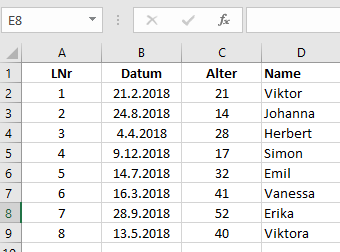
\includegraphics[width=0.30000\textwidth]{Images/ExcelTabelle.PNG}
\caption{\textbf{Abbildung 26}: Beispiel für unterschiedliche Daten in
einer Excel-Tabelle}
\end{figure}

In der ersten und dritten Spalte (LNr, Alter) sind numerische Werte, in
der zweiten ist ein Datum und in der vierten ein Name (String,
Charakters). Wärde diese Tabelle in R als Matrix gespeichert, würde R
alle Daten in den Datentyp \emph{character} umwandeln! Bei einem
\emph{Datenframe} wird im Gegensatz dazu der Datentyp jeder Spalte
beibehalten.

Um aus bestehenden Objekten (Vektoren, Matrizen) einen Datenframe zu
erstellen, wird die Funktion \emph{data.frame()} benutzt. Der Zugriff
auf die Elemente eines Dataframes ist gleich wie bei Matrizen. Der Name
des \emph{Dataframes} gefolgt von zwei eckigen Klammern, innerhalb
welcher die Indizes der Zeilen und Spalten angegeben werden.
Entsprechend kann auch die Bezeichnung der Spalten und Zeilen über die
Funktionen colnames() und rowname() angezeigt, bzw. verändert werden
(vgl. Matrizen).

Darüber hinaus bietet der Dataframe noch eine spezielle Form der
Adressierung von Spalten. Betrachtet man die Spalten als Variablen,
deren Namen durch den Spaltennamen gegeben ist, kann mittels folgender
Syntax auf die entsprechende Spalte zugegriffen werden:
\emph{DataframeName\$SpaltenName}. Die Adressierung von Elementen
innerhalb einer Variablen (Spalte) wird weiterhin mit der Indexmethode
durchgeführt.

Manche Programmierer bevorzugen einen \emph{schlanken Code}, d.h. es
soll so wenig wie möglich Text in den Programmzeilen stehen. Bei der
Verwendung von Dataframes gibt es die Funktionen
\emph{attach(DataframeName)} und \emph{detach(DataframeName}). Erstere
bewirkt, dass bei der Referenz auf Variablen eines Dataframes der Name
desselben nicht mehr angegeben werden muss (man spart sich also den
\emph{DataframeName\$}). Allerdings stehen dann die Inhalten nur mehr
zum Lesen zur Verfügung. Mit \emph{detach(DataFrameName)} wird die
direkte Referenzierung über Variablennamen wieder aufgehoben. Es sei
jedoch darauf hingewiesen, dass sich einige Probleme in Zusammenhang mit
der Benennung anderer Variablen ergeben können!

Folgender Code zeigt die soeben beschriebenen Eigenschaften. Kopiere den
Code in den Editor und führe diesen dann zeilenweise aus:

\begin{Shaded}
\begin{Highlighting}[]
\NormalTok{    A  <-}\StringTok{ }\DecValTok{1}\OperatorTok{:}\DecValTok{10}
\NormalTok{    B  <-}\StringTok{ }\KeywordTok{c}\NormalTok{(}\KeywordTok{rep}\NormalTok{(}\DecValTok{0}\NormalTok{,}\DecValTok{5}\NormalTok{), }\KeywordTok{rep}\NormalTok{(}\DecValTok{1}\NormalTok{,}\DecValTok{5}\NormalTok{))}
\NormalTok{    B  <-}\StringTok{ }\KeywordTok{factor}\NormalTok{(B, }\DataTypeTok{levels =} \KeywordTok{c}\NormalTok{(}\DecValTok{0}\NormalTok{,}\DecValTok{1}\NormalTok{), }\DataTypeTok{labels =} \KeywordTok{c}\NormalTok{(}\StringTok{"Male"}\NormalTok{, }\StringTok{"Female"}\NormalTok{))}
\NormalTok{    C  <-}\StringTok{ }\KeywordTok{c}\NormalTok{(}\StringTok{"Georg"}\NormalTok{, }\StringTok{"Hanna"}\NormalTok{, }\StringTok{"Belinda"}\NormalTok{, }\StringTok{"Christoph"}\NormalTok{, }\StringTok{"Claudia"}\NormalTok{, }
           \StringTok{"Peter"}\NormalTok{, }\StringTok{"Nikolas"}\NormalTok{, }\StringTok{"Eva"}\NormalTok{, }\StringTok{"Gerda"}\NormalTok{, }\StringTok{"August"}\NormalTok{)}
\NormalTok{    D  <-}\StringTok{ }\KeywordTok{sample}\NormalTok{(}\DecValTok{15}\OperatorTok{:}\DecValTok{93}\NormalTok{, }\DecValTok{10}\NormalTok{, }\DataTypeTok{replace =} \OtherTok{TRUE}\NormalTok{)}
    
\NormalTok{    E  <-}\StringTok{ }\KeywordTok{rbind}\NormalTok{(A, B, C, D) }\CommentTok{# Wandelt alle Daten in Character! Daher verwendet man die Funktion data.frame()}
    
\NormalTok{    DF <-}\StringTok{ }\KeywordTok{data.frame}\NormalTok{(A, B, C, D)}
    \KeywordTok{str}\NormalTok{(DF)               }\CommentTok{# Zeigt die Struktur und jeweiligen Datentypen in der Struktur Dataframe E}
\NormalTok{    DF}
\NormalTok{    DF[}\DecValTok{1}\NormalTok{,}\DecValTok{2}\NormalTok{]}
    \KeywordTok{colnames}\NormalTok{(DF)}
    \KeywordTok{rownames}\NormalTok{(DF)}
    \KeywordTok{colnames}\NormalTok{(DF) <-}\StringTok{ }\KeywordTok{c}\NormalTok{(}\StringTok{"LNr"}\NormalTok{, }\StringTok{"Geschlecht"}\NormalTok{, }\StringTok{"Name"}\NormalTok{,}\StringTok{"Alter"}\NormalTok{)}
\NormalTok{    AnzZeilenDF  <-}\StringTok{ }\KeywordTok{dim}\NormalTok{(DF)[}\DecValTok{1}\NormalTok{] }\CommentTok{# oder nrow(DF)}
    \KeywordTok{rownames}\NormalTok{(DF) <-}\StringTok{ }\KeywordTok{paste0}\NormalTok{(}\StringTok{"VP"}\NormalTok{, }\DecValTok{1}\OperatorTok{:}\NormalTok{AnzZeilenDF)}
    \KeywordTok{rownames}\NormalTok{(DF) <-}\StringTok{ }\KeywordTok{paste0}\NormalTok{(}\StringTok{"VP"}\NormalTok{, }\DecValTok{1}\OperatorTok{:}\KeywordTok{nrow}\NormalTok{(DF))    }\CommentTok{# gleichwertige M?glichkeit}
    \KeywordTok{rownames}\NormalTok{(DF) <-}\StringTok{ }\KeywordTok{paste0}\NormalTok{(}\StringTok{"VP"}\NormalTok{, }\DecValTok{1}\OperatorTok{:}\KeywordTok{dim}\NormalTok{(DF)[}\DecValTok{1}\NormalTok{])  }\CommentTok{# gleichwertige M?glichkeit}
\NormalTok{    DF}
\NormalTok{    DF}\OperatorTok{$}\NormalTok{Name}
\NormalTok{    DF}\OperatorTok{$}\NormalTok{Alter[}\DecValTok{2}\OperatorTok{:}\DecValTok{3}\NormalTok{]}
    \KeywordTok{attach}\NormalTok{(DF)}
\NormalTok{    Alter}
    \KeywordTok{detach}\NormalTok{(DF)}
\end{Highlighting}
\end{Shaded}

\subsubsection*{Aufgabenblock
Dataframes}\label{aufgabenblock-dataframes}
\addcontentsline{toc}{subsubsection}{Aufgabenblock Dataframes}

Verwende wiederum nachfolgende Daten zum Bearbeiten der Aufgaben:

\begin{Shaded}
\begin{Highlighting}[]
\NormalTok{    id     <-}\StringTok{ }\KeywordTok{c}\NormalTok{(}\DecValTok{11}\NormalTok{, }\DecValTok{16}\NormalTok{, }\DecValTok{17}\NormalTok{, }\DecValTok{18}\NormalTok{, }\DecValTok{19}\NormalTok{, }\DecValTok{20}\NormalTok{, }\DecValTok{23}\NormalTok{) }\CommentTok{# c() entspr. combine; <- Zuweisung zu einer Variablen}
\NormalTok{    Geschlecht <-}\StringTok{ }\KeywordTok{c}\NormalTok{(}\StringTok{"männlich"}\NormalTok{, }\StringTok{"weiblich"}\NormalTok{)}
\NormalTok{    sex    <-}\StringTok{ }\KeywordTok{c}\NormalTok{(}\DecValTok{1}\NormalTok{, }\DecValTok{1}\NormalTok{, }\DecValTok{7}\NormalTok{, }\DecValTok{1}\NormalTok{, }\DecValTok{1}\NormalTok{, }\DecValTok{2}\NormalTok{, }\DecValTok{2}\NormalTok{)}
\NormalTok{    lalt   <-}\StringTok{ }\KeywordTok{c}\NormalTok{(}\DecValTok{2}\NormalTok{, }\DecValTok{3}\NormalTok{, }\DecValTok{2}\NormalTok{, }\DecValTok{3}\NormalTok{, }\DecValTok{1}\NormalTok{, }\DecValTok{1}\NormalTok{, }\DecValTok{2}\NormalTok{)}
\NormalTok{    gross  <-}\StringTok{  }\KeywordTok{c}\NormalTok{(}\DecValTok{173}\NormalTok{, }\DecValTok{166}\NormalTok{, }\DecValTok{178}\NormalTok{, }\DecValTok{154}\NormalTok{, }\DecValTok{164}\NormalTok{, }\DecValTok{389}\NormalTok{, }\DecValTok{181}\NormalTok{)}
\NormalTok{    mon    <-}\StringTok{ }\KeywordTok{c}\NormalTok{(}\DecValTok{266}\NormalTok{, }\DecValTok{241}\NormalTok{, }\DecValTok{231}\NormalTok{, }\DecValTok{265}\NormalTok{, }\DecValTok{225}\NormalTok{, }\DecValTok{229}\NormalTok{, }\DecValTok{222}\NormalTok{)}
\NormalTok{    date   <-}\StringTok{ }\KeywordTok{c}\NormalTok{(}\DecValTok{4}\NormalTok{, }\DecValTok{5}\NormalTok{, }\DecValTok{3}\NormalTok{, }\DecValTok{3}\NormalTok{, }\DecValTok{2}\NormalTok{, }\DecValTok{4}\NormalTok{, }\DecValTok{3}\NormalTok{)}
\NormalTok{    entsch <-}\StringTok{ }\KeywordTok{c}\NormalTok{(}\DecValTok{3}\NormalTok{, }\DecValTok{4}\NormalTok{, }\DecValTok{4}\NormalTok{, }\DecValTok{5}\NormalTok{, }\DecValTok{3}\NormalTok{, }\DecValTok{1}\NormalTok{, }\DecValTok{2}\NormalTok{)}
\NormalTok{    proj   <-}\StringTok{ }\KeywordTok{c}\NormalTok{(}\DecValTok{2}\NormalTok{, }\DecValTok{1}\NormalTok{, }\DecValTok{2}\NormalTok{, }\DecValTok{2}\NormalTok{, }\DecValTok{2}\NormalTok{, }\DecValTok{1}\NormalTok{, }\DecValTok{2}\NormalTok{)}
\NormalTok{    i1     <-}\StringTok{ }\KeywordTok{c}\NormalTok{(}\DecValTok{3}\NormalTok{, }\DecValTok{2}\NormalTok{, }\DecValTok{1}\NormalTok{, }\DecValTok{3}\NormalTok{, }\DecValTok{4}\NormalTok{, }\DecValTok{2}\NormalTok{, }\DecValTok{2}\NormalTok{)}
\NormalTok{    i2     <-}\StringTok{ }\KeywordTok{c}\NormalTok{(}\DecValTok{3}\NormalTok{, }\DecValTok{2}\NormalTok{, }\DecValTok{1}\NormalTok{, }\DecValTok{3}\NormalTok{, }\DecValTok{4}\NormalTok{, }\DecValTok{2}\NormalTok{, }\DecValTok{2}\NormalTok{)}
\NormalTok{    i3     <-}\StringTok{ }\KeywordTok{c}\NormalTok{(}\DecValTok{3}\NormalTok{, }\DecValTok{3}\NormalTok{, }\DecValTok{3}\NormalTok{, }\DecValTok{2}\NormalTok{, }\DecValTok{2}\NormalTok{, }\DecValTok{2}\NormalTok{, }\DecValTok{4}\NormalTok{)}
\NormalTok{    i4     <-}\StringTok{ }\KeywordTok{c}\NormalTok{(}\DecValTok{2}\NormalTok{, }\DecValTok{1}\NormalTok{, }\DecValTok{2}\NormalTok{, }\DecValTok{4}\NormalTok{, }\DecValTok{2}\NormalTok{, }\DecValTok{1}\NormalTok{, }\DecValTok{4}\NormalTok{)}
\NormalTok{    i5     <-}\StringTok{ }\KeywordTok{c}\NormalTok{(}\DecValTok{2}\NormalTok{, }\DecValTok{1}\NormalTok{, }\DecValTok{4}\NormalTok{, }\DecValTok{1}\NormalTok{, }\DecValTok{3}\NormalTok{, }\DecValTok{4}\NormalTok{, }\DecValTok{1}\NormalTok{)}
\end{Highlighting}
\end{Shaded}

\begin{enumerate}
\def\labelenumi{\arabic{enumi}.}
\tightlist
\item
  erstelle eine Datenstruktur (data.frame) mit dem Namen
  \emph{fragebogen} mit folgenden Inhalt: \emph{id}, \emph{Geschlecht},
  \emph{sex}, \emph{lalt}, \emph{gross}, \emph{mon}, \emph{date},
  \emph{entsch}, \emph{proj}, \emph{i1}, \emph{i2}, \emph{i3},
  \emph{i4}, \emph{i5}
\item
  gib die 3te Zeile des \emph{fragebogens} aus.
\item
  verwende die Funktion \emph{head()} und diskutiere das Ergebnis
\item
  versuche den Befehl fragebogen\$i1{[}1:3{]}. Diskutieren sie das
  Ergebnis, sehen Sie nach was das \$ bedeutet!
\item
  gib die Werte der 1'ten bis zur 3'ten Zeile der Spalte \emph{proj}
  aus.
\item
  versuche den Befehl attach() und den Befehl detach(). Verwende bei
  Bedarfsfall die Hilfefunktion.
\end{enumerate}

\subsection*{Data-Tables}\label{data-tables}
\addcontentsline{toc}{subsection}{Data-Tables}

Eine erweiterte Version von \emph{Dataframes} wir durch das Paket
\emph{data.table}\footnote{Paket von Matt Dowle, kann über CRAN-Server
  geladen werden.}. Einer der wesentlichen Vorteile bei der Verwendung
von data.table liegt vor allem in der beträchtlich schnelleren
Verarbeitung - vor allem bei sehr großen Datensätzen. Das Paket
beinhaltet eine Funktion (fread()) zum Lesen von \emph{csv}-Dateien,
welche in Hinblick auf Ladezeiten sehr großer Dateien die oft verwendete
Funktion \emph{read.csv()} in den Schatten stellt. Auch die Handhabung
der Daten in einer \emph{data.table} ist bei weitem schneller als in
einem \emph{Dataframe}.

Trotz dieser Vorteile verzichten wir im Folgenden auf die Verwendung
dieser Funktionen, da wir einerseits nicht mit \emph{big data} arbeiten
werden und andererseits ein Großteil der von R zur Verfügung gestellten
Beispieldatensätze in Form von \emph{Dataframes} und \emph{Listen}
vorfinden werden.

\subsection*{Listen}\label{listen}
\addcontentsline{toc}{subsection}{Listen}

Um den Einschränkungen bezüglich der \emph{Dataframes} zu entgehen, kann
der Datentyp \emph{list} verwendet werden. List-Objekte können neben
verschiedenen Datentypen auch unterschiedlich große Objekte (Skalare,
Vektoren, Matrizen, Dataframes), aber Objektstrukturen wie z.B.
Funktionen beinhalten. Listen bilden damit eine Möglichkeit, so ziemlich
alles was in R an Objekten erzeugt werden kann in einer Variablen des
Typs list abzuspeichern. Eine Liste zu erzeugen erfolgt einfach über die
Funktion \emph{list()}. Betrachten wir zunächst folgenden Code:

\begin{Shaded}
\begin{Highlighting}[]
\NormalTok{    LI        <-}\StringTok{ }\KeywordTok{list}\NormalTok{(}\StringTok{"Rot"}\NormalTok{, }\KeywordTok{c}\NormalTok{(}\DecValTok{21}\NormalTok{,}\DecValTok{32}\NormalTok{,}\DecValTok{11}\NormalTok{), }\OtherTok{TRUE}\NormalTok{, }\FloatTok{51.23}\NormalTok{, m1) }\CommentTok{# Generiere Liste mit verschiedenen Eintr?gen}
    \KeywordTok{str}\NormalTok{(LI) }\CommentTok{# Zeige die Struktur der Liste an}
    \KeywordTok{names}\NormalTok{(LI) <-}\StringTok{ }\KeywordTok{c}\NormalTok{(}\StringTok{"Farbe"}\NormalTok{, }\StringTok{"Alter"}\NormalTok{, }\StringTok{"Raucher"}\NormalTok{,}\StringTok{"Gewicht"}\NormalTok{, }\StringTok{"Matrix"}\NormalTok{)}
    \KeywordTok{str}\NormalTok{(LI)}
    \CommentTok{# Alternativ kann man die Namen der Listen auch bereits bei der Erstellung durchf?hren}
\NormalTok{    LI1        <-}\StringTok{ }\KeywordTok{list}\NormalTok{(}\DataTypeTok{Farbe =} \StringTok{"Rot"}\NormalTok{, }
                       \DataTypeTok{Vec =} \KeywordTok{c}\NormalTok{(}\DecValTok{21}\NormalTok{,}\DecValTok{32}\NormalTok{,}\DecValTok{11}\NormalTok{), }
                       \DataTypeTok{Logi =} \OtherTok{TRUE}\NormalTok{, }
                       \DataTypeTok{Wert =} \FloatTok{51.23}\NormalTok{, }
                       \DataTypeTok{Mat =}\NormalTok{ m1) }\CommentTok{# Generiere Liste mit verschiedenen Eintr?gen}
    \KeywordTok{str}\NormalTok{(LI1)}
    
\NormalTok{    LI}\OperatorTok{$}\NormalTok{Farbe}
\NormalTok{    LI}\OperatorTok{$}\NormalTok{Matrix[}\DecValTok{2}\NormalTok{, }\DecValTok{2}\OperatorTok{:}\DecValTok{3}\NormalTok{]}
\NormalTok{    LI[}\DecValTok{5}\NormalTok{]}
\NormalTok{    LI[[}\DecValTok{5}\NormalTok{]][}\DecValTok{2}\NormalTok{, }\DecValTok{2}\OperatorTok{:}\DecValTok{3}\NormalTok{]}
    
\NormalTok{    LI[}\DecValTok{6}\NormalTok{] <-}\StringTok{ }\KeywordTok{list}\NormalTok{(}\DataTypeTok{Matrix2 =}\NormalTok{ m2) }\CommentTok{# F?ge Element als letztes Element der Liste hinzu}
    \KeywordTok{str}\NormalTok{(LI)}
\NormalTok{    LI[}\DecValTok{6}\NormalTok{] <-}\StringTok{ }\OtherTok{NULL} \CommentTok{# Entferne letztes Element der Liste}

\NormalTok{    LI    <-}\StringTok{ }\KeywordTok{list}\NormalTok{(LI, }\KeywordTok{list}\NormalTok{(}\StringTok{"green"}\NormalTok{,}\FloatTok{12.3}\NormalTok{)) }\CommentTok{# Listen ineinander verschachteln}
    \KeywordTok{str}\NormalTok{(LI) }\CommentTok{# Zeige die Struktur der Liste an}
\NormalTok{    LI[[}\DecValTok{1}\NormalTok{]]}\OperatorTok{$}\NormalTok{Farbe}
\NormalTok{    LI[[}\DecValTok{2}\NormalTok{]][}\DecValTok{1}\NormalTok{]}
\NormalTok{    XLi <-}\StringTok{ }\KeywordTok{unlist}\NormalTok{(LI)}
\NormalTok{    XLi}
\end{Highlighting}
\end{Shaded}

\subsection*{Tables}\label{tables}
\addcontentsline{toc}{subsection}{Tables}

Eine weitere Möglichkeit in R Daten in Objekten zu speichern bietet die
Klasse der \emph{Tables}. Die unterschiedlichen Formen der Tables sind
am besten durch folgende Beispiele zu erklären:

\begin{Shaded}
\begin{Highlighting}[]
    \KeywordTok{rm}\NormalTok{(}\DataTypeTok{list =} \KeywordTok{ls}\NormalTok{())}
\NormalTok{    F1 <-}\StringTok{ }\KeywordTok{factor}\NormalTok{(}\KeywordTok{c}\NormalTok{(}\StringTok{"A"}\NormalTok{,}\StringTok{"A"}\NormalTok{,}\StringTok{"B"}\NormalTok{,}\StringTok{"A"}\NormalTok{,}\StringTok{"B"}\NormalTok{,}\StringTok{"B"}\NormalTok{,}\StringTok{"C"}\NormalTok{,}\StringTok{"A"}\NormalTok{,}\StringTok{"C"}\NormalTok{))}
\NormalTok{    results <-}\StringTok{ }\KeywordTok{table}\NormalTok{(F1)}
\NormalTok{    results}
    \KeywordTok{attributes}\NormalTok{(F1)}
    
    
\NormalTok{    V1 <-}\StringTok{ }\KeywordTok{c}\NormalTok{(}\StringTok{"Sometimes"}\NormalTok{,}\StringTok{"Sometimes"}\NormalTok{,}\StringTok{"Never"}\NormalTok{,}\StringTok{"Always"}\NormalTok{,}\StringTok{"Always"}\NormalTok{,}\StringTok{"Sometimes"}\NormalTok{,}\StringTok{"Sometimes"}\NormalTok{,}\StringTok{"Never"}\NormalTok{)}
\NormalTok{    V2 <-}\StringTok{ }\KeywordTok{c}\NormalTok{(}\StringTok{"Maybe"}\NormalTok{,}\StringTok{"Maybe"}\NormalTok{,}\StringTok{"Yes"}\NormalTok{,}\StringTok{"Maybe"}\NormalTok{,}\StringTok{"Maybe"}\NormalTok{,}\StringTok{"No"}\NormalTok{,}\StringTok{"Yes"}\NormalTok{,}\StringTok{"No"}\NormalTok{)}
\NormalTok{    results <-}\StringTok{ }\KeywordTok{table}\NormalTok{(V1,V2)}
\NormalTok{    results    }
    
\NormalTok{    sexsmoke           <-}\StringTok{ }\KeywordTok{matrix}\NormalTok{(}\KeywordTok{c}\NormalTok{(}\DecValTok{70}\NormalTok{,}\DecValTok{120}\NormalTok{,}\DecValTok{65}\NormalTok{,}\DecValTok{140}\NormalTok{),}\DataTypeTok{ncol =} \DecValTok{2}\NormalTok{,}\DataTypeTok{byrow =} \OtherTok{TRUE}\NormalTok{)}
    \KeywordTok{rownames}\NormalTok{(sexsmoke) <-}\StringTok{ }\KeywordTok{c}\NormalTok{(}\StringTok{"male"}\NormalTok{,}\StringTok{"female"}\NormalTok{)}
    \KeywordTok{colnames}\NormalTok{(sexsmoke) <-}\StringTok{ }\KeywordTok{c}\NormalTok{(}\StringTok{"smoke"}\NormalTok{,}\StringTok{"nosmoke"}\NormalTok{)}
\NormalTok{    sexsmoke           <-}\StringTok{ }\KeywordTok{as.table}\NormalTok{(sexsmoke)}
\NormalTok{    sexsmoke}
    
\NormalTok{    sexsmoke_DF        <-}\StringTok{ }\KeywordTok{as.data.frame}\NormalTok{(sexsmoke)}
    
    \KeywordTok{library}\NormalTok{(data.table)}
    
\NormalTok{    DT <-}\StringTok{ }\KeywordTok{data.table}\NormalTok{( }\DataTypeTok{ID =} \DecValTok{1}\OperatorTok{:}\DecValTok{50}\NormalTok{,}
                      \DataTypeTok{Capacity =} \KeywordTok{sample}\NormalTok{(}\DecValTok{100}\OperatorTok{:}\DecValTok{1000}\NormalTok{, }\DataTypeTok{size =} \DecValTok{50}\NormalTok{, }\DataTypeTok{replace =}\NormalTok{ F),}
                      \DataTypeTok{Code =} \KeywordTok{sample}\NormalTok{(LETTERS[}\DecValTok{1}\OperatorTok{:}\DecValTok{4}\NormalTok{], }\DecValTok{50}\NormalTok{, }\DataTypeTok{replace =}\NormalTok{ T),}
                      \DataTypeTok{State =} \KeywordTok{rep}\NormalTok{(}\KeywordTok{c}\NormalTok{(}\StringTok{"Alabama"}\NormalTok{,}\StringTok{"Indiana"}\NormalTok{,}\StringTok{"Texas"}\NormalTok{,}\StringTok{"Nevada"}\NormalTok{), }\DecValTok{50}\NormalTok{))}
    
    \CommentTok{#simple data.table command}
\NormalTok{    DT[Code }\OperatorTok{==}\StringTok{ "C"}\NormalTok{, }\KeywordTok{mean}\NormalTok{(Capacity), State]}
    
\NormalTok{    DT[Code }\OperatorTok{==}\StringTok{ "D"}\NormalTok{]}
\NormalTok{    DT[, }\KeywordTok{mean}\NormalTok{(Capacity), by =}\StringTok{ }\NormalTok{State]}
\NormalTok{    DT[Code }\OperatorTok{==}\StringTok{ "A"}\NormalTok{, }\KeywordTok{mean}\NormalTok{(Capacity)]}
\end{Highlighting}
\end{Shaded}

Tabellen können mit der Funktion \emph{as.data.frame(tbl)} leicht in die
bereits bekannte Klasse des Datenframes umgewandelt werden.

\subsection*{Attribute}\label{attribute}
\addcontentsline{toc}{subsection}{Attribute}

Allen bisher besprochenen Objekte in R können beliebige zusätzlichen
Eigenschaften (Attribute) zugewiesen werden. Attribute kann man sich als
Namenslisten vorstellen, welche durch die Funktion \emph{attr()}
festgelegt werden können.

\begin{Shaded}
\begin{Highlighting}[]
    \KeywordTok{str}\NormalTok{(sexsmoke)}
    \KeywordTok{attr}\NormalTok{(sexsmoke, }\StringTok{"dim"}\NormalTok{)}
    
\NormalTok{    y <-}\StringTok{ }\DecValTok{1}\OperatorTok{:}\DecValTok{10}
    \KeywordTok{attr}\NormalTok{(y, }\StringTok{"Mein_Attribut"}\NormalTok{) <-}\StringTok{ "y ist ein Vektor"}
    
    \KeywordTok{attr}\NormalTok{(y, }\StringTok{"Mein_Attribut"}\NormalTok{)}
    \KeywordTok{str}\NormalTok{(}\KeywordTok{attributes}\NormalTok{(y))}
\end{Highlighting}
\end{Shaded}

Auf den Umgang und die Verwendung von Attributen wird in folgenden
Kapiteln entsprechend verwiesen. Vor allem beim Import von Daten (z.B.
SPSS Ergebnisse einer Limesurveyumfrage) können die Attribute für die
Speicherung zu Metainformation einer Variablen (Itemformulierung zu
einer Variablen) sehr hilfreich sein.

\begin{center}\rule{0.5\linewidth}{\linethickness}\end{center}

\subsection*{Lösungen}\label{losungen-1}
\addcontentsline{toc}{subsection}{Lösungen}

\subsubsection*{Lösungen zu Aufgabenblock Copy und
Paste}\label{losungen-zu-aufgabenblock-copy-und-paste}
\addcontentsline{toc}{subsubsection}{Lösungen zu Aufgabenblock Copy und
Paste}

\begin{Shaded}
\begin{Highlighting}[]
  \CommentTok{# Aufgabe 1}
\NormalTok{    v <-}\StringTok{ }\KeywordTok{c}\NormalTok{(}\DecValTok{1}\NormalTok{,}\DecValTok{4}\NormalTok{,}\DecValTok{4}\NormalTok{,}\DecValTok{3}\NormalTok{,}\DecValTok{2}\NormalTok{,}\DecValTok{2}\NormalTok{,}\DecValTok{3}\NormalTok{)}
  \CommentTok{# Aufgabe 2}
\NormalTok{    v[}\KeywordTok{c}\NormalTok{(}\DecValTok{2}\NormalTok{,}\DecValTok{3}\NormalTok{,}\DecValTok{4}\NormalTok{)]}
  \CommentTok{# Aufgabe 3}
\NormalTok{    dat <-}\StringTok{ }\KeywordTok{data.frame}\NormalTok{(}
      \DataTypeTok{time =} \KeywordTok{factor}\NormalTok{(}\KeywordTok{c}\NormalTok{(}\StringTok{"Lunch"}\NormalTok{,}\StringTok{"Dinner"}\NormalTok{), }\DataTypeTok{levels =} \KeywordTok{c}\NormalTok{(}\StringTok{"Lunch"}\NormalTok{,}\StringTok{"Dinner"}\NormalTok{)),}
      \DataTypeTok{total_bill =} \KeywordTok{c}\NormalTok{(}\FloatTok{14.89}\NormalTok{, }\FloatTok{17.23}\NormalTok{)}
\NormalTok{    )}
\NormalTok{    dat}
    \CommentTok{#>     time total_bill}
    \CommentTok{#> 1  Lunch      14.89}
    \CommentTok{#> 2 Dinner      17.23}
  \CommentTok{# Aufgabe 4 & 5}
    \KeywordTok{library}\NormalTok{(ggplot2)}\CommentTok{# Load the ggplot2 package}
    \CommentTok{# Very basic bar graph}
    \KeywordTok{ggplot}\NormalTok{(}\DataTypeTok{data=}\NormalTok{dat, }\KeywordTok{aes}\NormalTok{(}\DataTypeTok{x =}\NormalTok{ time, }\DataTypeTok{y =}\NormalTok{ total_bill)) }\OperatorTok{+}
\StringTok{      }\KeywordTok{geom_bar}\NormalTok{(}\DataTypeTok{stat=}\StringTok{"identity"}\NormalTok{)}
    \CommentTok{# Map the time of day to different fill colors}
    \KeywordTok{ggplot}\NormalTok{(}\DataTypeTok{data=}\NormalTok{dat, }\KeywordTok{aes}\NormalTok{(}\DataTypeTok{x =}\NormalTok{ time, }\DataTypeTok{y =}\NormalTok{ total_bill, }\DataTypeTok{fill =}\NormalTok{ time)) }\OperatorTok{+}
\StringTok{      }\KeywordTok{geom_bar}\NormalTok{(}\DataTypeTok{stat =} \StringTok{"identity"}\NormalTok{)}
\NormalTok{    ## This would have the same result as above}
    \CommentTok{# ggplot(data=dat, aes(x=time, y=total_bill)) +}
    \CommentTok{#    geom_bar(aes(fill=time), stat="identity")}
    \CommentTok{# Add a black outline}
    \KeywordTok{ggplot}\NormalTok{(}\DataTypeTok{data =}\NormalTok{ dat, }\KeywordTok{aes}\NormalTok{(}\DataTypeTok{x =}\NormalTok{ time, }\DataTypeTok{y =}\NormalTok{ total_bill, }\DataTypeTok{fill =}\NormalTok{ time)) }\OperatorTok{+}
\StringTok{      }\KeywordTok{geom_bar}\NormalTok{(}\DataTypeTok{colour =} \StringTok{"black"}\NormalTok{, }\DataTypeTok{stat =} \StringTok{"identity"}\NormalTok{)}
    \CommentTok{# No legend, since the information is redundant}
    \KeywordTok{ggplot}\NormalTok{(}\DataTypeTok{data=}\NormalTok{dat, }\KeywordTok{aes}\NormalTok{(}\DataTypeTok{x=}\NormalTok{time, }\DataTypeTok{y =}\NormalTok{ total_bill, }\DataTypeTok{fill =}\NormalTok{ time)) }\OperatorTok{+}
\StringTok{      }\KeywordTok{geom_bar}\NormalTok{(}\DataTypeTok{colour =} \StringTok{"black"}\NormalTok{, }\DataTypeTok{stat =} \StringTok{"identity"}\NormalTok{) }\OperatorTok{+}
\StringTok{      }\KeywordTok{guides}\NormalTok{(}\DataTypeTok{fill =} \OtherTok{FALSE}\NormalTok{)}
  \CommentTok{# Aufgabe 6}
    \KeywordTok{data}\NormalTok{()}
\NormalTok{    ?tips}
\NormalTok{    ?french_fries}
  \CommentTok{# Aufgabe 7}
\NormalTok{    Dat_FF <-}\StringTok{ }\NormalTok{french_fries}
    \KeywordTok{str}\NormalTok{(Dat_FF)}
  \CommentTok{# Aufgabe 8}
    \KeywordTok{library}\NormalTok{(haven)}
\NormalTok{    bigfive <-}\StringTok{ }\KeywordTok{read_sav}\NormalTok{(}\StringTok{"Data/bigfive.sav"}\NormalTok{)}
    \KeywordTok{View}\NormalTok{(bigfive)}
  \CommentTok{# Aufgabe 9}
    \KeywordTok{library}\NormalTok{(readxl)}
\NormalTok{    bigfive <-}\StringTok{ }\KeywordTok{read_excel}\NormalTok{(}\StringTok{"Data/bigfive.xls"}\NormalTok{)}
    \KeywordTok{View}\NormalTok{(bigfive)}
\end{Highlighting}
\end{Shaded}

\subsubsection*{Lösungen zu Aufgabenblock
Vektoren}\label{losungen-zu-aufgabenblock-vektoren}
\addcontentsline{toc}{subsubsection}{Lösungen zu Aufgabenblock Vektoren}

\begin{Shaded}
\begin{Highlighting}[]
    \KeywordTok{mean}\NormalTok{(gross)          }\CommentTok{# A1: Aufruf der Funktion mean().}
\NormalTok{    gross1     <-}\StringTok{  }\NormalTok{gross }\CommentTok{# A2: Kopiere Werte von gross in gross1}
\NormalTok{    gross1[}\DecValTok{1}\NormalTok{]  <-}\StringTok{  }\OtherTok{NA}    \CommentTok{# A3: setzte den ersten Wert von gross1 auf NA (not available) = missing value}
    \KeywordTok{mean}\NormalTok{(gross1)         }\CommentTok{# A4: BEACHTE, dass mean nun NA ist -> Markiere mean und dr?cke F1}
    \KeywordTok{mean}\NormalTok{(gross1, }\DataTypeTok{na.rm =} \OtherTok{TRUE}\NormalTok{) }\CommentTok{# A5: nun wird der Mittelwert richtig berechnet!}
    \KeywordTok{mean}\NormalTok{(gross1, }\DataTypeTok{trim =} \FloatTok{0.5}\NormalTok{, }\DataTypeTok{na.rm =} \OtherTok{TRUE}\NormalTok{) }\CommentTok{# A6}
\NormalTok{    gross_prod <-}\StringTok{ }\NormalTok{gross[}\DecValTok{2}\NormalTok{]}\OperatorTok{*}\NormalTok{gross[}\DecValTok{3}\NormalTok{] }\CommentTok{# A7}
\NormalTok{    sex[}\DecValTok{3}\NormalTok{]  <-}\StringTok{ }\DecValTok{1}    \CommentTok{# A8}
\NormalTok{    x       <-}\StringTok{ }\DecValTok{50}\OperatorTok{:}\DecValTok{1} \CommentTok{# A9}
\NormalTok{    x[}\OperatorTok{-}\DecValTok{2}\NormalTok{]           }\CommentTok{# A10: Alle Werte bis auf den zweiten Wert der Liste.}
\NormalTok{    x       <-}\StringTok{ }\KeywordTok{seq}\NormalTok{(}\DataTypeTok{from =} \DecValTok{1}\NormalTok{, }\CommentTok{# A11: vgl. gegebenenfalls in der Hilfe unter seq()}
                   \DataTypeTok{to =} \DecValTok{10}\NormalTok{,}
                   \DataTypeTok{by =} \DecValTok{2}\NormalTok{)}
\NormalTok{    x       <-}\StringTok{ }\KeywordTok{seq}\NormalTok{(}\DataTypeTok{from =} \DecValTok{10}\NormalTok{, }\CommentTok{# A12}
                   \DataTypeTok{to =} \DecValTok{2}\NormalTok{,}
                   \DataTypeTok{by =} \OperatorTok{-}\DecValTok{2}\NormalTok{)}
\NormalTok{    x       <-}\StringTok{ }\KeywordTok{c}\NormalTok{(}\KeywordTok{seq}\NormalTok{(}\DataTypeTok{from =} \DecValTok{0}\NormalTok{, }\CommentTok{# A13}
                     \DataTypeTok{to   =} \DecValTok{10}\NormalTok{,}
                     \DataTypeTok{by =} \DecValTok{2}\NormalTok{), }\DecValTok{50}\NormalTok{)}
    \KeywordTok{class}\NormalTok{(x)  }\CommentTok{# A14}
\NormalTok{    x_c <-}\StringTok{ }\KeywordTok{as.character}\NormalTok{(x) }\CommentTok{# A15}
    \KeywordTok{class}\NormalTok{(x_c) }\CommentTok{# A16}
\NormalTok{    x_n <-}\StringTok{ }\KeywordTok{as.numeric}\NormalTok{(x)  }\CommentTok{# A17}
    \KeywordTok{class}\NormalTok{(x_n) }\CommentTok{# A18}
    \KeywordTok{sum}\NormalTok{(gross }\OperatorTok{>=}\StringTok{ }\DecValTok{173}\NormalTok{) }\CommentTok{# A19}
    \KeywordTok{which}\NormalTok{(gross }\OperatorTok\StringTok{ }\DecValTok{181}\NormalTok{) }\CommentTok{# A20}
\end{Highlighting}
\end{Shaded}

\subsubsection*{Lösungen zu Aufgabenblock
Faktoren}\label{losungen-zu-aufgabenblock-faktoren}
\addcontentsline{toc}{subsubsection}{Lösungen zu Aufgabenblock Faktoren}

\begin{Shaded}
\begin{Highlighting}[]
    \CommentTok{# Aufgabe 1}
\NormalTok{    x       <-}\StringTok{ }\KeywordTok{c}\NormalTok{(}\DecValTok{1}\NormalTok{, }\DecValTok{2}\NormalTok{, }\DecValTok{3}\NormalTok{, }\DecValTok{1}\NormalTok{, }\DecValTok{1}\NormalTok{, }\DecValTok{2}\NormalTok{, }\DecValTok{2}\NormalTok{)}
\NormalTok{    x_fact  <-}\StringTok{ }\KeywordTok{factor}\NormalTok{(x, }\DataTypeTok{levels =} \KeywordTok{c}\NormalTok{(}\DecValTok{1}\NormalTok{, }\DecValTok{2}\NormalTok{, }\DecValTok{3}\NormalTok{), }\DataTypeTok{labels =} \KeywordTok{c}\NormalTok{(}\StringTok{'A'}\NormalTok{, }\StringTok{'B'}\NormalTok{, }\StringTok{'C'}\NormalTok{))}
    \CommentTok{# Aufgabe 2}
\NormalTok{    x_fact2         <-}\StringTok{ }\NormalTok{x_fact}
    \KeywordTok{levels}\NormalTok{(x_fact2) <-}\StringTok{ }\KeywordTok{c}\NormalTok{(}\StringTok{'S1'}\NormalTok{, }\StringTok{'S2'}\NormalTok{, }\StringTok{'S3'}\NormalTok{)}
    \KeywordTok{table}\NormalTok{(x_fact2)}
    \CommentTok{# Aufgabe 3}
\NormalTok{    x_fact3 <-}\StringTok{ }\KeywordTok{factor}\NormalTok{(x_fact2, }\DataTypeTok{levels =} \KeywordTok{c}\NormalTok{(}\StringTok{"S3"}\NormalTok{, }\StringTok{"S1"}\NormalTok{, }\StringTok{"S2"}\NormalTok{))}
    \KeywordTok{table}\NormalTok{(x_fact2)}
    \KeywordTok{table}\NormalTok{(x_fact3)}
\end{Highlighting}
\end{Shaded}

\subsubsection*{Lösungen zu Aufgabenblock
Matrizen}\label{losungen-zu-aufgabenblock-matrizen}
\addcontentsline{toc}{subsubsection}{Lösungen zu Aufgabenblock Matrizen}

\begin{Shaded}
\begin{Highlighting}[]
\NormalTok{    X <-}\StringTok{ }\KeywordTok{cbind}\NormalTok{(lalt, sex, gross) }\CommentTok{# A1}
\NormalTok{    Z <-}\StringTok{ }\KeywordTok{rbind}\NormalTok{(lalt, sex, gross) }\CommentTok{# A2}
\NormalTok{    X[}\DecValTok{2}\NormalTok{,}\DecValTok{3}\NormalTok{] }\CommentTok{# A3}
\NormalTok{    X[}\DecValTok{3}\NormalTok{,] }\CommentTok{# A4}
\NormalTok{    X[}\DecValTok{3}\OperatorTok{:}\DecValTok{5}\NormalTok{,}\DecValTok{1}\OperatorTok{:}\DecValTok{2}\NormalTok{]  }\CommentTok{# A5}
    \KeywordTok{colnames}\NormalTok{(X)  }\CommentTok{# A6}
\NormalTok{    ColNames    <-}\StringTok{ }\KeywordTok{c}\NormalTok{(}\StringTok{"Alter"}\NormalTok{, }\StringTok{"Gewicht"}\NormalTok{, }\StringTok{"Gr??e"}\NormalTok{)  }\CommentTok{# A7}
    \KeywordTok{colnames}\NormalTok{(X) <-}\StringTok{ }\NormalTok{ColNames }\CommentTok{# A8}
\NormalTok{    namen       <-}\StringTok{ }\KeywordTok{c}\NormalTok{(}\StringTok{"Walter"}\NormalTok{, }\StringTok{"Gerda"}\NormalTok{,}\StringTok{"Hannes"}\NormalTok{, }\StringTok{"Ute"}\NormalTok{, }\StringTok{"Hanna"}\NormalTok{,}\StringTok{"Doris"}\NormalTok{,}\StringTok{"Karin"}\NormalTok{) }\CommentTok{# A9}
    \KeywordTok{rownames}\NormalTok{(X) <-}\StringTok{ }\NormalTok{namen  }\CommentTok{# A10}
    \KeywordTok{fix}\NormalTok{(X)  }\CommentTok{# A11}
    \KeywordTok{dim}\NormalTok{(X)  }\CommentTok{# A12}
    \KeywordTok{length}\NormalTok{(X)  }\CommentTok{# A13}
    \KeywordTok{cbind}\NormalTok{(X, X[,}\DecValTok{3}\NormalTok{] }\OperatorTok{/}\StringTok{ }\DecValTok{100}\NormalTok{)}
    \KeywordTok{which}\NormalTok{(X[,}\DecValTok{3}\NormalTok{] }\OperatorTok{>}\StringTok{ }\DecValTok{200}\NormalTok{)}
\end{Highlighting}
\end{Shaded}

\subsubsection*{Lösungen zu Aufgabenblock
Dataframes}\label{losungen-zu-aufgabenblock-dataframes}
\addcontentsline{toc}{subsubsection}{Lösungen zu Aufgabenblock
Dataframes}

\begin{Shaded}
\begin{Highlighting}[]
\NormalTok{    fragebogen <-}\StringTok{ }\KeywordTok{data.frame}\NormalTok{(id, sex, lalt, gross, mon, date, entsch, proj, i1, i2, i3, i4, i5) }\CommentTok{# A1}
\NormalTok{    fragebogen[}\DecValTok{3}\NormalTok{,] }\CommentTok{# A2}
    \KeywordTok{head}\NormalTok{(fragebogen) }\CommentTok{# A3}
\NormalTok{    fragebogen}\OperatorTok{$}\NormalTok{i1[}\DecValTok{1}\OperatorTok{:}\DecValTok{3}\NormalTok{] }\CommentTok{# A4}
\NormalTok{    fragebogen[}\DecValTok{1}\OperatorTok{:}\DecValTok{3}\NormalTok{,}\DecValTok{9}\NormalTok{] }\CommentTok{# A5}
\NormalTok{    fragebogen[}\DecValTok{1}\OperatorTok{:}\DecValTok{3}\NormalTok{,}\StringTok{"i1"}\NormalTok{] }\CommentTok{# A5 - Alternative L?ung mit Verwendung des Spaltennamens}
    \KeywordTok{attach}\NormalTok{(fragebogen) }\CommentTok{# A6}
    \KeywordTok{detach}\NormalTok{(fragebogen) }\CommentTok{# A6}
\end{Highlighting}
\end{Shaded}

\section{Rarbeiten}\label{rarbeiten}

Unabhängig vom verwendeten Statistik-Programm werden wir in den meisten
Fällen Daten nicht erst im jeweiligen Programm definieren und erfassen,
sondern auf bereits vorliegende Daten zurückgreifen. Eine wichtige
Ausnahme ist dabei die Simulation von Daten. Bereits mit einem
\emph{normalen} Desktop-PC ist es möglich, eine Unmenge an Daten
(surrogate data) im Handumdrehen zu erzeugen und diese mittels
statistischer Verfahren, Modelle und Algorithmen innerhalb kürzester
Zeit auszuwerten. Zur Prüfung der Eigenschaften von Modellen und
Algorithmen ist diese Vorgehensweise ein wichtiges Hilfsmittel.

Zur Erfassung von Echtdaten wird aber üblicherweise kein statistisches
Analyseprogramm verwendet. Daher liegen diese Daten auch in
verschiedensten Formaten vor und es ist einer der ersten Schritte in der
statistischen Datenanalyse, diese Daten vom jeweiligen Format in ein für
das Statistikprogramm lesbares umzuwandeln. Die am häufigsten
verwendeten Formate mit denen wir es derzeit zu tun haben sind:

\begin{itemize}
\tightlist
\item
  R-Dateien im \emph{RData}, \emph{rda} und \emph{rds} Format
\item
  Textdateien im \emph{csv}, \emph{dat}, \emph{txt} Format
\item
  SPSS, JAMOVI, etc. Dateien (\emph{sav}, \emph{omv}, etc.)
\item
  Excel-Tabellen im xls, oder \emph{xlsx} Format
\item
  Binäre Daten im \emph{bin} Format
\item
  Proprietäre Formate diverser Labor- und Messgeräte
\end{itemize}

Im Folgenden beschränken wir uns auf die üblichsten Fileformate, den R-,
Text-, SPSS- und Excel-Dateien.

\subsection*{Lesen und speichern von
Dateien}\label{lesen-und-speichern-von-dateien}
\addcontentsline{toc}{subsection}{Lesen und speichern von Dateien}

Das Lesen und Speichern von Dateien kann entweder direkt im RStudio über
das Environment-Pane, oder über einen entsprechenden R-Code in der
Konsole, bzw. über den Source-Pane durchgeführt werden. Zu unterscheiden
sind die verschiedenen Dateitypen, von denen es abhängt, welche Funktion
zu wählen ist.

\subsubsection*{R-Dateien}\label{r-dateien}
\addcontentsline{toc}{subsubsection}{R-Dateien}

Liegen Daten bereits im R-eigenen Format vor, können diese einfach mit
der Funktion \emph{load(Dateiname)} eingelesen werden. Bezüglich der
Dateierweiterung unterscheidet R folgende Typen:

\begin{enumerate}
\def\labelenumi{\arabic{enumi}.}
\tightlist
\item
  \emph{.RData}: der Inhalt des zum Zeitpunkt des speicherns
  (\emph{save()}) vorhandenen Environments.
\item
  \emph{.rda}: Kurzbezeichnung für RData.
\item
  \emph{.rds}: speichert ein einzelnes R-Objekt.
\end{enumerate}

Der Vorteil dieser Datenformate liegt darin, dass die Datenstrukturen,
wie z.B. Datentypen der Spalten (numerisch, character, factor) erhalten
bleiben. Bei anderen Dateiformaten ist dies nicht automatisch gegeben.
In einem ersten Schritt verwenden wir die im Environment-Pane
vorhandenen Möglichkeiten Files zu laden und zu speichern.

Kopiere zuerst den nachfolgenden Code in ein neues R-Script, speicher
dieses unter dem Namen \emph{07\_RArbeiten\_Files.R} und führe
anschließen den Code zeilenweise aus.

\begin{Shaded}
\begin{Highlighting}[]
\CommentTok{# Initialisierung}
  \KeywordTok{rm}\NormalTok{(}\DataTypeTok{list =} \KeywordTok{ls}\NormalTok{())}
  \ControlFlowTok{if}\NormalTok{ (}\OperatorTok{!}\KeywordTok{require}\NormalTok{(}\StringTok{"pacman"}\NormalTok{)) }\KeywordTok{install.packages}\NormalTok{(}\StringTok{"pacman"}\NormalTok{)}
\NormalTok{  pacman}\OperatorTok{::}\KeywordTok{p_load}\NormalTok{(here)}
  \CommentTok{# Ende Initialisierung}
\end{Highlighting}
\end{Shaded}

Verwende nun das Symbol \emph{Open File} im Environment-Pane und wähle
die Datei \emph{bigfive.RData} im entsprechenden Datenverzeichnis
(gegebenenfalls noch von
\href{http://tuval.at/lehrveranstaltungen/daten/data}{Daten zum Seminar}
herunterladen und lokal am Rechner speichern). Führe folgende
Arbeitsschritte durch:

\begin{enumerate}
\def\labelenumi{\arabic{enumi}.}
\tightlist
\item
  Im Konsolenfenster wird die Funktion zum Laden der Datei
  (\emph{load(xxx)}) angezeigt. Kopier diese Zeile in den Editor.
\item
  Erzeuge eine Kopie dieses Objektes und benenne diese mit
  \emph{KopieBigFive}
\item
  Verwende das Symbol Speichern im Environment-Pane und speichere den
  Inhalt des Environments unter den Namen \emph{BigFive\_New\_1}. Im
  Konsolenfenster wird die Funktion zum Speichern der Datei
  (\emph{save.image(xxx)}) angezeigt. Kopier diese Zeile in den Editor.
  Ruf die Hilfefunktion auf um herauszufinden, was es mit dieser
  Funktion auf sich hat.
\item
  Bereinige das Environment unter Verwendung des Pinsel-Symbol.
\item
  Lade die soeben gespeicherte Datei (\emph{BigFive\_New\_1.RData}) mit
  dem Symbol \emph{Open File}. Beachte, dass nun beide Objekte wieder im
  Environment zur Verfügung stehen.
\end{enumerate}

Nachfolgender Code zeigt die soeben besprochenen Aufgabenschritte.

\begin{Shaded}
\begin{Highlighting}[]
  \KeywordTok{load}\NormalTok{(}\KeywordTok{here}\NormalTok{(}\StringTok{"Data/bigfive.RData"}\NormalTok{)) }\CommentTok{# A1}
\NormalTok{  KopieBigFive <-}\StringTok{ }\NormalTok{bigfive  }\CommentTok{# A2}
  \KeywordTok{save.image}\NormalTok{(}\KeywordTok{here}\NormalTok{(}\StringTok{"Data/BigFive_1.RData"}\NormalTok{))  }\CommentTok{# A3}
  \KeywordTok{rm}\NormalTok{(}\DataTypeTok{list =} \KeywordTok{ls}\NormalTok{()) }\CommentTok{# A4}
  \KeywordTok{load}\NormalTok{(}\KeywordTok{here}\NormalTok{(}\StringTok{"Data/BigFive_1.RData"}\NormalTok{)) }\CommentTok{# A5}
  \KeywordTok{save.image}\NormalTok{(}\KeywordTok{here}\NormalTok{(}\StringTok{"Data/BigFive_2.RData"}\NormalTok{)) }\CommentTok{# A6}
  \KeywordTok{rm}\NormalTok{(}\DataTypeTok{list =} \KeywordTok{ls}\NormalTok{()) }\CommentTok{# A7}
  \KeywordTok{load}\NormalTok{(}\KeywordTok{here}\NormalTok{(}\StringTok{"Data/BigFive_2.RData"}\NormalTok{)) }\CommentTok{# A8}
  
  \KeywordTok{saveRDS}\NormalTok{(KopieBigFive, }\DataTypeTok{file =} \KeywordTok{here}\NormalTok{(}\StringTok{"Data/BigFive_3.rds"}\NormalTok{))}
  \KeywordTok{rm}\NormalTok{(}\DataTypeTok{list =} \KeywordTok{ls}\NormalTok{())}
\NormalTok{  KopieBigFive <-}\StringTok{ }\KeywordTok{readRDS}\NormalTok{( }\KeywordTok{here}\NormalTok{(}\StringTok{"Data/BigFive_3.rds"}\NormalTok{) )}
\end{Highlighting}
\end{Shaded}

Im folgenden werden ergänzende Möglichkeiten zum Speichern/Laden von
Daten gezeigt. Mit der Funktion saveRDS() können einzelne Objekte
gespeichert und mit readRDS() auch wieder geladen werden. Will man
mehrere, aber nicht alle Objekte des Environments speichern, kann dies
durch Angabe der Objektnamen und der Funktion save() durchgeführt
werden.

\begin{Shaded}
\begin{Highlighting}[]
\NormalTok{  Seminar <-}\StringTok{ "R-Intro"}
\NormalTok{  V1      <-}\StringTok{ }\DecValTok{1}\OperatorTok{:}\DecValTok{10}
\NormalTok{  M1      <-}\StringTok{ }\KeywordTok{matrix}\NormalTok{(}\DecValTok{1}\NormalTok{, }\DecValTok{3}\NormalTok{, }\DecValTok{3}\NormalTok{)}
\NormalTok{  M2      <-}\StringTok{ }\KeywordTok{matrix}\NormalTok{(}\DecValTok{5}\NormalTok{, }\DecValTok{8}\NormalTok{, }\DecValTok{3}\NormalTok{)}
  
  \KeywordTok{save}\NormalTok{(Seminar, V1, }\DataTypeTok{file =} \KeywordTok{here}\NormalTok{(}\StringTok{"Data/BigFive_4.RData"}\NormalTok{) )}
  \KeywordTok{rm}\NormalTok{(}\DataTypeTok{list =} \KeywordTok{ls}\NormalTok{())}
  \KeywordTok{load}\NormalTok{(}\KeywordTok{here}\NormalTok{(}\StringTok{"Data/BigFive_4.RData"}\NormalTok{))}
  \KeywordTok{rm}\NormalTok{(}\DataTypeTok{list =} \KeywordTok{ls}\NormalTok{())}
\end{Highlighting}
\end{Shaded}

\subsubsection*{Text-Dateien}\label{text-dateien}
\addcontentsline{toc}{subsubsection}{Text-Dateien}

Mit der \emph{read.csv()}, \emph{read.table()} und verwandten Funktionen
können Daten aus Textdateien (txt) importiert werden.
\emph{read.table()} ist die Basisfunktion zum Import von Textdateien.
\emph{read.csv()} und \emph{read.csv2()} sowie einige andere Funktionen
sind Anpassungen an häufig auftretenden Fülle.

CSV\footnote{\emph{C}omma \emph{S}eparated \emph{V}alues} ist für viele
Tabellenkalkulationen und andere Anwendungen ein übliches Exportformat.
Irreführend bei diesem Format ist oftmals die Verwendung der
Trennzeichen für unterschiedliche Daten. Der Name \emph{csv} suggeriert,
dass ein Kommazeichen die Datensätze innerhalb der Datei trennt.
Tatsächlich kann man aber ein beliebiges Zeichen verwenden. Am
häufigsten findet man den Tabulator, oder den Strichpunkt als
Trennzeichen. Bezüglich des Kommazeichens sollte man noch vor dem Import
einer Datei prüfen, ob dieses als Trennzeichen für Dezimalzahlen
verwendet wurde, oder ob (wie im englischen Sprachraum üblich) der Punkt
die Dezimaltrennung kennzeichnet.

Bemerkung bezüglich der Leistungsfähigkeit von Funktionen beim Lesen von
(wirklich) großen Dateien: die \emph{read.csv()} und damit verwandten
Funktionen weisen bei \emph{big data} im Vergleich zu optimierten
Funktionen wie z.B. \emph{fread()} (aus dem Paket \emph{data.table})
wesentlich höhere Ladezeiten auf. Bei kleinen Datensätzen ist dies
jedoch zu vernachlässigen.

Um eine Textdatei zu laden, betrachten wir zunächst wie RStudio dabei
vorgeht. Im Environment-Pane finden wir bei den Reitern die Möglichkeit
\emph{Import-Dataset}. Folgende Optionen werden angeboten:

\begin{itemize}
\tightlist
\item
  From Text (base) \ldots{}
\item
  From Text (readr) \ldots{}
\item
  From SPSS \ldots{}
\item
  From Excel \ldots{}
\item
  From SAS \ldots{}
\item
  From Stata \ldots{}
\end{itemize}

Lade die Datei \emph{ATM.txt} mit der Option \emph{From Text (base)
\ldots{}} und kopiere die Befehlszeilen in den Editor. Diskutiere die
Ergebnisse. Entferne anschließend alle Inhalte aus dem Environment und
wiederhole das Laden der Datei mit der Option \emph{From Text (readr)
\ldots{}}. Vergleiche die Funktionen und diskutiere den Unterschied der
beiden Funktionen.

\begin{Shaded}
\begin{Highlighting}[]
\NormalTok{  ATM <-}\StringTok{ }\KeywordTok{read.delim}\NormalTok{(}\StringTok{"C:/NextCloud/LEHRE2019/18WS R-Intro/Data/ATM.txt"}\NormalTok{)}
  \KeywordTok{View}\NormalTok{(ATM)  }
  
  \KeywordTok{rm}\NormalTok{(}\DataTypeTok{list =} \KeywordTok{ls}\NormalTok{())}
  
  \KeywordTok{library}\NormalTok{(readr)}
\NormalTok{  ATM <-}\StringTok{ }\KeywordTok{read_table2}\NormalTok{(}\StringTok{"Data/ATM.txt"}\NormalTok{)}
  \KeywordTok{View}\NormalTok{(ATM)}
\end{Highlighting}
\end{Shaded}

\subsubsection*{SPSS-Dateien}\label{spss-dateien}
\addcontentsline{toc}{subsubsection}{SPSS-Dateien}

Wie bei den Textdateien, verwenden wir in einem ersten Schritt die
Importfunktion von RStudio. Lade die Datei \emph{bigfive.sav} (eine SPSS
Datei) und kopiere den Code aus der Konsole in den Editor.

\begin{Shaded}
\begin{Highlighting}[]
  \KeywordTok{rm}\NormalTok{(}\DataTypeTok{list =} \KeywordTok{ls}\NormalTok{())}
  \KeywordTok{library}\NormalTok{(haven)}
\NormalTok{  bigfive <-}\StringTok{ }\KeywordTok{read_sav}\NormalTok{(}\StringTok{"Data/bigfive.sav"}\NormalTok{)}
  \KeywordTok{View}\NormalTok{(bigfive)}
  \KeywordTok{str}\NormalTok{(bigfive)}
\end{Highlighting}
\end{Shaded}

Überprüfe die Struktur des geladenen Objektes. Auffallend ist der
bislang noch nicht besprochenen Datentyp \emph{tbl\_df}. Dabei handelt
es sich im Wesentlichen um einen Dataframe. Gehe in den Files-Pane zu
den Packages und suche nach dem Paket \emph{haven}. Öffne die Doku des
Pakets, bzw. öffne die Hilfe zu \emph{haven::read\_sav()} direkt.
Weiterführend Information zu diesem Datenformat ist unter anderem auf
folgender Seite zu finden: \href{https://tibble.tidyverse.org/}{Tibble}

Eine weitere - zum Einlesen von SPSS-Dateien - geeignete Funktion wird
im Paket \emph{foreign} angeboten (\emph{read.spss()}).

Aufgabe:

\begin{enumerate}
\def\labelenumi{\arabic{enumi}.}
\tightlist
\item
  Stelle fest, ob in deinem Repository dieses Paket bereits geladen ist
  (\emph{Hinweis}: vgl.
  \href{https://www.r-bloggers.com/list-of-user-installed-r-packages-and-their-versions/}{List
  of Packages}). Falls nicht, lade das Paket samt abhängigen Paketen.
\item
  Bereinigen das Environment und lade die Datei \emph{bigfive.sav} mit
  Hilfe der Funktion \emph{read.spss()}.
\item
  Überprüfe und diskutiere den Inhalt, bzw. die Datentypen des geladenen
  Objektes.
\end{enumerate}

\begin{Shaded}
\begin{Highlighting}[]
\NormalTok{  ip           <-}\StringTok{ }\KeywordTok{as.data.frame}\NormalTok{(}\KeywordTok{installed.packages}\NormalTok{()[,}\KeywordTok{c}\NormalTok{(}\DecValTok{1}\NormalTok{,}\DecValTok{3}\OperatorTok{:}\DecValTok{4}\NormalTok{)])}
  \KeywordTok{rownames}\NormalTok{(ip) <-}\StringTok{ }\OtherTok{NULL}
\NormalTok{  ip           <-}\StringTok{ }\NormalTok{ip[}\KeywordTok{is.na}\NormalTok{(ip}\OperatorTok{$}\NormalTok{Priority),}\DecValTok{1}\OperatorTok{:}\DecValTok{2}\NormalTok{, drop =}\StringTok{ }\OtherTok{FALSE}\NormalTok{]}
  \KeywordTok{print}\NormalTok{(ip, }\DataTypeTok{row.names =} \OtherTok{FALSE}\NormalTok{)}
  \KeywordTok{library}\NormalTok{(foreign)  }
\NormalTok{  BF           <-}\StringTok{ }\KeywordTok{read.spss}\NormalTok{(}\StringTok{"Data/bigfive.sav"}\NormalTok{, }\DataTypeTok{to.data.frame =} \OtherTok{TRUE}\NormalTok{)}
  \KeywordTok{str}\NormalTok{(BF)}
\end{Highlighting}
\end{Shaded}

Neben den Paketen \emph{haven} und \emph{foreign} gibt es noch weitere
Packages welche Funktionen zum Einlesen von SPSS-Dateien beinhalten
(z.B. \emph{Hmisc} mit der Funktion \emph{spss.get()}). Die derzeit
wahrscheinlich beste Funktion ist im Paket \emph{haven} zu finden, aber
auch alle anderen Funktionen aus anderen Packages erfüllen i.A. ihren
Zweck.

\subsubsection*{Excel-Dateien}\label{excel-dateien}
\addcontentsline{toc}{subsubsection}{Excel-Dateien}

Das Laden und Speichern von Excel-Dateien sollte aufgrund der Häufigkeit
mit der Daten aus diesem Programm in R übernommen werden keine Hexerei
sein. Erfahrungsgemäß ist aber gerade dieses Format (\emph{xls} und
\emph{xlsx}) nicht so einfach zu handhaben wie zu erwarten wäre.

Die einfachste (und oft durchgeführte Alternative) ist die Speicherung
von \emph{xls}-Tabellen als \emph{csv}-Dateien. Anderenfalls gibt es
natürlich verschiedene Packages mit Funktionen die derartige Dateien
direkt lesen und schreiben können. Folgende Packages enthalten
Funktionen zum Lesen von Excel-Files:

\begin{itemize}
\tightlist
\item
  \emph{readxl} (kann nur Excel-Dateien lesen, nicht schreiben)
\item
  \emph{xlsx}
\item
  \emph{XLConnect}
\item
  \emph{gdata} u.v.m.
\end{itemize}

Die Entscheidung, welches davon genutzt wird, bleibt dem Anwender
überlassen. RStudio verwendet im Import das \emph{readxl}. Zum
Kennenlernen werden wir in einem ersten Schritt die Datei
\emph{bigfive\_excel.xls} über den Datenimport von RStudio laden. Bitte
den entsprechenden Code in den Editor kopieren. Anschließend testen wir
die Funktion des Packages \emph{xlsx}. Für die Verwendung von
\emph{XLConnect} und \emph{gdata} sei aus zeitlichen Gründen auf die
entsprechende Dokumentation verwiesen.

Neben dem Einlesen von Excel-Files ist das Speichern von Ergebnissen in
Excelformat für die weitere Verwendung des Endnutzers sehr wichtig. Wie
Daten in ein Excelfile übertragen und dieses auch abgespeichert wird,
ist dem nachfolgenden Code zu entnehmen. Kopiere den Code in den Editor
und führe diesen zeilenweise aus. Diskutiere die Ergebnisse.

\begin{Shaded}
\begin{Highlighting}[]
  \KeywordTok{rm}\NormalTok{(}\DataTypeTok{list =} \KeywordTok{ls}\NormalTok{())}
  
  \KeywordTok{library}\NormalTok{(readxl)}
\NormalTok{    ptm <-}\StringTok{ }\KeywordTok{proc.time}\NormalTok{()}
\NormalTok{    bigfive_excel_}\DecValTok{1}\NormalTok{ <-}\StringTok{ }\NormalTok{readxl}\OperatorTok{::}\KeywordTok{read_excel}\NormalTok{(}\StringTok{"Data/bigfive_excel.xls"}\NormalTok{) }\CommentTok{# Funktion prüft ob xls oder xlsx}
    \KeywordTok{proc.time}\NormalTok{() }\OperatorTok{-}\StringTok{ }\NormalTok{ptm}
    \KeywordTok{str}\NormalTok{(bigfive_excel_}\DecValTok{1}\NormalTok{)  }
\NormalTok{    bigfive_excel_}\DecValTok{2}\NormalTok{ <-}\StringTok{ }\NormalTok{readxl}\OperatorTok{::}\KeywordTok{read_xls}\NormalTok{(}\StringTok{"Data/bigfive_excel.xls"}\NormalTok{) }\CommentTok{# Funktion lädt nur xls Format}
\NormalTok{    bigfive_excel_}\DecValTok{3}\NormalTok{ <-}\StringTok{ }\NormalTok{readxl}\OperatorTok{::}\KeywordTok{read_xlsx}\NormalTok{(}\StringTok{"Data/bigfive_excel.xlsx"}\NormalTok{) }\CommentTok{# Funktion lädt nur xlsx Format}

  \KeywordTok{library}\NormalTok{(xlsx)}
\NormalTok{    ptm <-}\StringTok{ }\KeywordTok{proc.time}\NormalTok{()}
\NormalTok{    bigfive_excel_}\DecValTok{4}\NormalTok{ <-}\StringTok{ }\NormalTok{xlsx}\OperatorTok{::}\KeywordTok{read.xlsx}\NormalTok{(}\StringTok{"Data/bigfive_excel.xlsx"}\NormalTok{, }\DataTypeTok{sheetIndex =} \DecValTok{1}\NormalTok{)}
    \KeywordTok{proc.time}\NormalTok{() }\OperatorTok{-}\StringTok{ }\NormalTok{ptm}
    
    \KeywordTok{write.xlsx}\NormalTok{(bigfive_excel_}\DecValTok{4}\NormalTok{, }
               \StringTok{"Data/bigfive_excel_Write.xlsx"}\NormalTok{, }
               \DataTypeTok{sheetName =} \StringTok{"Datenblatt"}\NormalTok{, }
               \DataTypeTok{col.names =} \OtherTok{TRUE}\NormalTok{, }
               \DataTypeTok{row.names =} \OtherTok{TRUE}\NormalTok{, }
               \DataTypeTok{append    =} \OtherTok{FALSE}\NormalTok{, }
               \DataTypeTok{showNA    =} \OtherTok{TRUE}\NormalTok{, }
               \DataTypeTok{password  =} \OtherTok{NULL}\NormalTok{)}
\end{Highlighting}
\end{Shaded}

\emph{Bemerkung zu Excel-Packages}: neben den oben angeführten Packages
existieren noch einige weitere, die Funktionen mit Excel-Read-Write
anbieten. Manche verlangen Java, andere Perl-Scripts. Einige sind
spezialisiert auf effizienten Zugriff und der Bearbeitung von Zellen,
andere sind extrem schnell beim Laden von großen Dateien. Üblicherweise
reichen die beiden vorgestellten Pakete.

\subsubsection*{Dateien vom Web}\label{dateien-vom-web}
\addcontentsline{toc}{subsubsection}{Dateien vom Web}

Die verschiedensten Dateiformate können auch von einer Website oder eine
FTP-Server geladen werden. Nachfolgend ein Beispiel, wie eine Datei
direkt von einem Server eingelesen werden kann.

\begin{Shaded}
\begin{Highlighting}[]
\NormalTok{    WebData <-}\StringTok{ }\KeywordTok{read.table}\NormalTok{(}\StringTok{"http://www.tuval.at/wp-content/uploads/Airquality.txt"}\NormalTok{, }\DataTypeTok{header =} \OtherTok{FALSE}\NormalTok{)}
\end{Highlighting}
\end{Shaded}

\section{Rechnen mit R}\label{rechnen-mit-r}

\subsection*{Deskriptive Datenanalyse}\label{deskriptive-datenanalyse}
\addcontentsline{toc}{subsection}{Deskriptive Datenanalyse}

Ziel einer deskriptiven Analyse ist eine möglichst genaue Beschreibung
von Daten mit einer möglichst kleinen Menge an Zahlen. Dazu eignen sich
vor allem:

\begin{itemize}
\tightlist
\item
  Kennwerte
\item
  Tabellen
\item
  Graphiken
\end{itemize}

Mit der deskriptiven Analyse ist es darüber hinaus möglich, Daten auf
ihre Plausibilität und Richtigkeit zu prüfen. Die Bedeutung einer
genauen deskriptiven Analyse und die korrekte Interpretation der
Ergebnisse dieser Analyse kann nicht hoch genug eingeschätzt werden.

Liegen erst einmal Daten vor ist es entweder zu schwierig, aufwendig,
oder zu spät am Versuchsdesign noch etwas nachträglich zu ändern.
Allerdings kann man mit einer sorgsamen deskriptiven Analyse durchaus
grobe Fehler bei der weiteren Analyse mit statistischen Verfahren
vermeiden. Eine der wichtigsten Erkenntnisse für jeden Datenanalytiker
ist, dass schlechte Daten nur schlechte Ergebnisse liefern können
(garbage in - garbage out Problem). Daher sind vor Beginn jeder
statistischen Analyse von Daten die deskriptiven Analysen unerlässlich.

Folgende Kapitel versuchen einen groben Überblick über die Möglichkeiten
der deskriptiven Analyse mit R zu geben. Da es diesbezüglich bereits
eine sehr große Anzahl an guten Paketen mit sehr vielen hilfreichen
Funktionen gibt, ist es im Rahmen dieser LV unmöglich auf alle Details
einzugehen. Unser Streifzug durch die deskriptive Statistik mit R ist
somit als Anstoß und Motivation für weitere, selbstständig
durchzuführende Studien zu diesem Thema zu sehen.

\subsubsection*{Kennwerte der deskriptiven
Statistik}\label{kennwerte-der-deskriptiven-statistik}
\addcontentsline{toc}{subsubsection}{Kennwerte der deskriptiven
Statistik}

Kennwerte der deskriptiven Statistik lassen sich bezüglich der
Beschreibung der Häufigkeiten, zentralen Tendenzen,
Verteilungseigenschaften und der Dispersion unterteilen.

\begin{itemize}
\tightlist
\item
  \emph{Häufigkeiten}
\item
  \emph{Zentrale Tendenzen}: Mittelwert, Median, Modus
\item
  \emph{Verteilungseigenschaften}: Schiefe (skew), Breite (kurtosis),
  Minimum, Maximum
\item
  \emph{Dispersion}: Spannweite, Quantile, Varianz, Standardabweichung,
  Standardfehler.
\end{itemize}

Für die meisten der genannten Kennwerte gibt es im R-Basispaket
entsprechende Funktionen. Manche der Funktionen (z.B. Schiefe und
Kurtosis) sind in Paketen (z.B. \emph{moments}) verfügbar. Der
Standardfehler kann ebenfalls in einem Paket (z.B. plotrix mit Funktion
\emph{std.error()}) berechnet werden. Da die Berechnung jedoch sehr
einfach ist, kann man sich hier selbst schnell mit einer Funktion
behelfen.

Aufgabe: programmiere die Berechnung des Standardfehlers als Funktion.
Der Standardfehler berechnet sich:

\(SE = \frac{s_x}{\sqrt{N}}\) oder \(SE = \sqrt{\frac{s^2_x}{N}}\)

\emph{Bemerkung}: verwende die \emph{Extract Function (Ctrl Alt X)} für
die Erstellung der Funktion.

\begin{Shaded}
\begin{Highlighting}[]
  \KeywordTok{table}\NormalTok{(DF}\OperatorTok{$}\NormalTok{geschlecht)}
  \KeywordTok{mean}\NormalTok{(DF}\OperatorTok{$}\NormalTok{alter)}
  \KeywordTok{median}\NormalTok{(DF}\OperatorTok{$}\NormalTok{alter)}
  
  \KeywordTok{skewness}\NormalTok{(DF}\OperatorTok{$}\NormalTok{alter)}
  \KeywordTok{agostino.test}\NormalTok{(DF}\OperatorTok{$}\NormalTok{alter, }\DataTypeTok{alternative =} \KeywordTok{c}\NormalTok{(}\StringTok{"two.sided"}\NormalTok{))}
  \KeywordTok{kurtosis}\NormalTok{(DF}\OperatorTok{$}\NormalTok{alter)}
  \KeywordTok{anscombe.test}\NormalTok{(DF}\OperatorTok{$}\NormalTok{alter, }\DataTypeTok{alternative =} \KeywordTok{c}\NormalTok{(}\StringTok{"two.sided"}\NormalTok{))}

  \KeywordTok{min}\NormalTok{(DF}\OperatorTok{$}\NormalTok{alter)}
  \KeywordTok{max}\NormalTok{(DF}\OperatorTok{$}\NormalTok{alter)    }
  \KeywordTok{range}\NormalTok{(DF}\OperatorTok{$}\NormalTok{alter)  }
  \KeywordTok{quantile}\NormalTok{(DF}\OperatorTok{$}\NormalTok{alter)  }
  \KeywordTok{var}\NormalTok{(DF}\OperatorTok{$}\NormalTok{alter)  }
  \KeywordTok{sd}\NormalTok{(DF}\OperatorTok{$}\NormalTok{alter)}
  \CommentTok{# Hier den Code f?r den Standardfehler einbauen}
\end{Highlighting}
\end{Shaded}

Eine nützliche Funktion ist \emph{summary(mydata)}. Darüber hinaus
stehen zahlreiche Pakete für die Erstellung deskriptiver Statistiken zur
Verfügung. Nachfolgend eine Auswahl von Paketen:

\begin{itemize}
\tightlist
\item
  \emph{Hmisc}
\item
  \emph{pastecs}
\item
  \emph{psych}
\item
  \emph{doBy}
\end{itemize}

\begin{Shaded}
\begin{Highlighting}[]
  \KeywordTok{summary}\NormalTok{(DF)}
  \KeywordTok{summary}\NormalTok{(DF}\OperatorTok{$}\NormalTok{alter)}
  
\NormalTok{  pacman}\OperatorTok{::}\KeywordTok{p_load}\NormalTok{(doBy, Hmisc, pastecs, psych)}
  
\NormalTok{  Hmisc}\OperatorTok{::}\KeywordTok{describe}\NormalTok{(DF}\OperatorTok{$}\NormalTok{alter) }
\NormalTok{  pastecs}\OperatorTok{::}\KeywordTok{stat.desc}\NormalTok{(DF}\OperatorTok{$}\NormalTok{alter)}
\NormalTok{  psych}\OperatorTok{::}\KeywordTok{describe}\NormalTok{(DF}\OperatorTok{$}\NormalTok{alter)}
\NormalTok{  psych}\OperatorTok{::}\KeywordTok{describeBy}\NormalTok{(DF}\OperatorTok{$}\NormalTok{alter, }
                     \DataTypeTok{group =}\NormalTok{ DF}\OperatorTok{$}\NormalTok{geschlecht)}
\NormalTok{  doBy}\OperatorTok{::}\KeywordTok{summaryBy}\NormalTok{(alter }\OperatorTok{+}\StringTok{ }\NormalTok{BMI }\OperatorTok{~}\StringTok{ }\NormalTok{med }\OperatorTok{+}\StringTok{ }\NormalTok{geschlecht, }
                  \DataTypeTok{data =}\NormalTok{ DF,}
                  \DataTypeTok{FUN =} \ControlFlowTok{function}\NormalTok{(x) \{ }\KeywordTok{c}\NormalTok{(}\DataTypeTok{m =} \KeywordTok{mean}\NormalTok{(x), }
                                        \DataTypeTok{s =} \KeywordTok{sd}\NormalTok{(x)) \} )}
\end{Highlighting}
\end{Shaded}

Jedes dieser Pakete beinhaltet eine Vielzahl nützlicher Funktionen, die
im Rahmen dieses Kurses nicht besprochen werden können. Um zumindest den
Einblick in die Vielfalt der Funktionen eines Paketes zu erhalten, öffne
die Hilfe für das Paket \emph{Hmisc} und blättere durch den alphabetisch
sortierten Funktionsumfang des Paketes - sehr beeindrucken, oder?

\subsection*{Graphiken der deskriptiven
Statistik}\label{graphiken-der-deskriptiven-statistik}
\addcontentsline{toc}{subsection}{Graphiken der deskriptiven Statistik}

Graphiken sind die beste Form der Darstellung von Ergebnissen! Es wird
nicht immer möglich sein, entsprechende Graphiken zu erstellen, aber
wenn möglich, sollten Ergebnisse immer durch Graphen dargestellt werden!
In RStudio werden die Ergebnisse einer Grafikfunktion im Files-Pane
unter Plots ausgegeben.

\subsubsection*{Graphen des Basispakets}\label{graphen-des-basispakets}
\addcontentsline{toc}{subsubsection}{Graphen des Basispakets}

Das Basispaket von R bietet einige nützliche Grafikfunktionen, die sich
für eine einfache Darstellung von Daten bestens eignen. Diese sind:

\begin{itemize}
\tightlist
\item
  plot() - Standardfunktion zum Erstellen von Diagrammen
\item
  hist() - Erstellen von Histogrammen
\item
  pie() - Erstellen von Kreisdiagrammen
\item
  barplot() - Erstellen von Säulendiagrammen
\item
  boxplot() - Erstellen von Boxplots (beinhaltet: Maximalwert,
  Minimalwert, Median, Quartile, Ausreißer)
\item
  dotchart() - Erstellen von Punktdiagrammen
\end{itemize}

\begin{Shaded}
\begin{Highlighting}[]
  \CommentTok{# plot() function}
  \KeywordTok{plot}\NormalTok{(DF}\OperatorTok{$}\NormalTok{BMI, }\DataTypeTok{type =} \StringTok{"s"}\NormalTok{, }\DataTypeTok{main =} \StringTok{"BMI"}\NormalTok{)}
  \KeywordTok{points}\NormalTok{(DF}\OperatorTok{$}\NormalTok{BMI, }\DataTypeTok{cex =}\NormalTok{ .}\DecValTok{5}\NormalTok{, }\DataTypeTok{col =} \StringTok{"dark red"}\NormalTok{)  }
  \CommentTok{# hist() function}
  \KeywordTok{hist}\NormalTok{(DF}\OperatorTok{$}\NormalTok{BMI,}
       \DataTypeTok{breaks =} \DecValTok{20}\NormalTok{,}
       \DataTypeTok{main =} \StringTok{"Altersverteilung"}\NormalTok{,}
       \DataTypeTok{xlab =} \StringTok{"Alter in Jahren"}\NormalTok{,}
       \DataTypeTok{ylab =} \StringTok{"H?ufigkeiten"}\NormalTok{)}
  \CommentTok{# pie() function}
\NormalTok{  AK_Graph <-}\StringTok{ }\KeywordTok{table}\NormalTok{(DF}\OperatorTok{$}\NormalTok{ak)}
  \KeywordTok{pie}\NormalTok{(AK_Graph, }\DataTypeTok{radius =} \FloatTok{0.6}\NormalTok{)}
  \CommentTok{# barplot() function}
\NormalTok{  BMI_Graph <-}\StringTok{ }\KeywordTok{summaryBy}\NormalTok{(BMI }\OperatorTok{~}\StringTok{ }\NormalTok{ak, DF)}
  \KeywordTok{barplot}\NormalTok{(BMI_Graph}\OperatorTok{$}\NormalTok{BMI.mean)}
  \CommentTok{# boxplot() function}
  \KeywordTok{boxplot}\NormalTok{(DF}\OperatorTok{$}\NormalTok{BMI }\OperatorTok{~}\StringTok{ }\NormalTok{DF}\OperatorTok{$}\NormalTok{ak)}
  \CommentTok{# dotchart() function}
  \KeywordTok{dotchart}\NormalTok{(BMI_Graph}\OperatorTok{$}\NormalTok{BMI.mean, }
           \DataTypeTok{labels =}\NormalTok{ BMI_Graph}\OperatorTok{$}\NormalTok{ak)}
\end{Highlighting}
\end{Shaded}

Speziellere Graphiken können mit folgenden Funktionen dargestellt
werden:

\begin{itemize}
\tightlist
\item
  contour() - Erstellen von Konturdiagrammen, plotten von Isolinien
\item
  forestplot - (aus dem Zusatzpaket ``rmeta'') erzeugt ein so genanntes
  ``Forest Plot'' zusammen mit einer Texttabelle.
\item
  map - (aus dem Paket ``maps'' und ``mapdata'') erstellt Karten von
  Ländern, Kontinenten und der Welt
\item
  metaplot - (aus dem Zusatzpaket ``rmeta'') erzeugt ein so genanntes
  ``Forest Plot'' (Meta-Analyse-Plot), welches im Rahmen von
  Metaanalysen gängig ist.
\item
  persp() - Erstellen von Dreidimensionalen Abbildungen
\end{itemize}

Zur Bearbeitung von Details innerhalb von Graphiken stehen z.B. folgende
Funktionen zur Verfügung:

\begin{itemize}
\tightlist
\item
  par() - Setzen von grafischen Parametern
\item
  title() - Beschriftung von Diagrammen
\end{itemize}

Alle Graphiken die in R erzeugt werden, können in den verschiedensten
Dateiformaten abgespeichert werden:

\begin{itemize}
\tightlist
\item
  jpeg() - speichert die Grafik als jpeg-Datei ab.
\item
  png() - speichert die Grafik als png-Datei ab.
\item
  pdf() - speichert eine Grafik als PDF-Datei ab.
\item
  postscript() - Speichert die Grafikausgabe in eine Postscript-Datei.
\item
  savePlot() - Speichert die aktuelle Grafik in eine Datei
\item
  devSVG() - speichert eine Grafik als SVG-Datei ab. Dazu ist das
  Zusatzpaket RSvgDevice erforderlich.
\end{itemize}

\subsubsection*{Graphen mit ggplot2}\label{graphen-mit-ggplot2}
\addcontentsline{toc}{subsubsection}{Graphen mit ggplot2}

Mit dem Paket \emph{ggplot2} erweitern sich die Möglichkeiten bei der
Erstellung und Gestaltung von Graphiken erheblich. Es gehört zu den
mächtigsten und umfangreichsten Pakten zur Erstellung von Grafiken.
Gerade wegen dieser Eigenschaft kann es vor allem für Einsteiger oft
schwierig werden. Das Paket bietet aber die Einsteigerfunktion
\emph{qplot()} (für Quick Plot). Für Standardgraphiken ist diese
Funktion sehr hilfreich, denn viele der komplexen Möglichkeiten in
\emph{ggplot2} bleiben bei dieser Funktion verborgen.

Basierend auf den Grundlagen des Buches
\href{http://ggplot2.org/resources/2007-past-present-future.pdf}{The
grammar of graphics} von Leland Wilkinson baute Wickham sein
\href{http://en.wikipedia.org/wiki/Ggplot2}{Datenvisualisierungspaket}
auf und übernahm die grundlegenden Thesen des Buches, die auch heute
noch als richtungsweisend für die Statistik gelten. Laut Leland lässt
sich jeder Datensatz, egal welcher Komplexität, leicht darstellen, wenn
man ihn sinnvoll in \emph{Ästhetik} und \emph{Geometrie} unterteilt.
Mittels dieser Differenzierung können Aufgabenbereiche getrennt und
Zuständigkeiten an verschiedene Aspekte des Plots übergeben werden.

Sobald komplexere Daten visualisiert werden sollen, zeigen sich die
Vorteile von ggplot2:

\begin{itemize}
\tightlist
\item
  \emph{feste Schema}: jeder Plot kann/muss nach einem Muster
  abgearbeitet werden. Das fährt unter anderem dazu, dass der Code meist
  sehr einfach gehalten ist und bei nachträglichen Änderungen nur
  wenigen Abwandlungen unterzogen werden muss.
\item
  \emph{Farb- oder Formeinsatz}: innerhalb des Plots wird automatisch
  eine Legende berechnet, die ebenfalls jederzeit manuell gestaltbar
  ist. Dies steht ganz im Gegensatz zu R nativen Plots, die durchweg
  individuell durchprogrammiert werden müssen.
\item
  \emph{zeitsparend}
\end{itemize}

\paragraph{Quick Plot mit ggplot2}\label{quick-plot-mit-ggplot2}
\addcontentsline{toc}{paragraph}{Quick Plot mit ggplot2}

Die \emph{qplot()}-Funktion folgt nicht dem typischen
\emph{ggplot2}-Schema und ist eher als Einstieg ins Plotting gedacht,
ermöglicht jedoch dieselbe Plotvisualisierung wie die
\emph{ggplot()}-Funktion. Ihr Aufbau und ihre Gestaltung wird lediglich
durch verschiedenste Parameter bestimmt.

Öffne folgenden Link
\href{https://www.statmethods.net/advgraphs/ggplot2.html}{Quick Plot
Einstieg} und kopiere den Code der nach dem Text \emph{Here are some
examples using automotive data \ldots{}} folgt in den Editor. Weiter
nützliche Hinweise zu Quick Plot findest du unter Um
\href{http://ggplot2.org/book/qplot.pdf}{Quick Plot Cheat Sheet}.

\begin{Shaded}
\begin{Highlighting}[]
\NormalTok{  pacman}\OperatorTok{::}\KeywordTok{p_load}\NormalTok{(ggplot2)}
  
  \CommentTok{# create factors with value labels}
\NormalTok{  mtcars}\OperatorTok{$}\NormalTok{gear <-}\StringTok{ }\KeywordTok{factor}\NormalTok{(mtcars}\OperatorTok{$}\NormalTok{gear,}\DataTypeTok{levels=}\KeywordTok{c}\NormalTok{(}\DecValTok{3}\NormalTok{,}\DecValTok{4}\NormalTok{,}\DecValTok{5}\NormalTok{),}
                        \DataTypeTok{labels=}\KeywordTok{c}\NormalTok{(}\StringTok{"3gears"}\NormalTok{,}\StringTok{"4gears"}\NormalTok{,}\StringTok{"5gears"}\NormalTok{))}
\NormalTok{  mtcars}\OperatorTok{$}\NormalTok{am <-}\StringTok{ }\KeywordTok{factor}\NormalTok{(mtcars}\OperatorTok{$}\NormalTok{am,}\DataTypeTok{levels=}\KeywordTok{c}\NormalTok{(}\DecValTok{0}\NormalTok{,}\DecValTok{1}\NormalTok{),}
                      \DataTypeTok{labels=}\KeywordTok{c}\NormalTok{(}\StringTok{"Automatic"}\NormalTok{,}\StringTok{"Manual"}\NormalTok{))}
\NormalTok{  mtcars}\OperatorTok{$}\NormalTok{cyl <-}\StringTok{ }\KeywordTok{factor}\NormalTok{(mtcars}\OperatorTok{$}\NormalTok{cyl,}\DataTypeTok{levels=}\KeywordTok{c}\NormalTok{(}\DecValTok{4}\NormalTok{,}\DecValTok{6}\NormalTok{,}\DecValTok{8}\NormalTok{),}
                       \DataTypeTok{labels=}\KeywordTok{c}\NormalTok{(}\StringTok{"4cyl"}\NormalTok{,}\StringTok{"6cyl"}\NormalTok{,}\StringTok{"8cyl"}\NormalTok{))}
  
  \CommentTok{# Kernel density plots for mpg}
  \CommentTok{# grouped by number of gears (indicated by color)}
  \KeywordTok{qplot}\NormalTok{(mpg, }\DataTypeTok{data=}\NormalTok{mtcars, }\DataTypeTok{geom=}\StringTok{"density"}\NormalTok{, }\DataTypeTok{fill=}\NormalTok{gear, }\DataTypeTok{alpha=}\KeywordTok{I}\NormalTok{(.}\DecValTok{5}\NormalTok{),}
        \DataTypeTok{main=}\StringTok{"Distribution of Gas Milage"}\NormalTok{, }\DataTypeTok{xlab=}\StringTok{"Miles Per Gallon"}\NormalTok{,}
        \DataTypeTok{ylab=}\StringTok{"Density"}\NormalTok{)}
  
  \CommentTok{# Scatterplot of mpg vs. hp for each combination of gears and cylinders}
  \CommentTok{# in each facet, transmittion type is represented by shape and color}
  \KeywordTok{qplot}\NormalTok{(hp, mpg, }\DataTypeTok{data=}\NormalTok{mtcars, }\DataTypeTok{shape=}\NormalTok{am, }\DataTypeTok{color=}\NormalTok{am,}
        \DataTypeTok{facets=}\NormalTok{gear}\OperatorTok{~}\NormalTok{cyl, }\DataTypeTok{size=}\KeywordTok{I}\NormalTok{(}\DecValTok{3}\NormalTok{),}
        \DataTypeTok{xlab=}\StringTok{"Horsepower"}\NormalTok{, }\DataTypeTok{ylab=}\StringTok{"Miles per Gallon"}\NormalTok{)}
  
  \CommentTok{# Separate regressions of mpg on weight for each number of cylinders}
  \KeywordTok{qplot}\NormalTok{(wt, mpg, }\DataTypeTok{data=}\NormalTok{mtcars, }\DataTypeTok{geom=}\KeywordTok{c}\NormalTok{(}\StringTok{"point"}\NormalTok{, }\StringTok{"smooth"}\NormalTok{),}
        \DataTypeTok{method=}\StringTok{"lm"}\NormalTok{, }\DataTypeTok{formula=}\NormalTok{y}\OperatorTok{~}\NormalTok{x, }\DataTypeTok{color=}\NormalTok{cyl,}
        \DataTypeTok{main=}\StringTok{"Regression of MPG on Weight"}\NormalTok{,}
        \DataTypeTok{xlab=}\StringTok{"Weight"}\NormalTok{, }\DataTypeTok{ylab=}\StringTok{"Miles per Gallon"}\NormalTok{)}
  
  \CommentTok{# Boxplots of mpg by number of gears}
  \CommentTok{# observations (points) are overlayed and jittered}
  \KeywordTok{qplot}\NormalTok{(gear, mpg, }\DataTypeTok{data=}\NormalTok{mtcars, }\DataTypeTok{geom=}\KeywordTok{c}\NormalTok{(}\StringTok{"boxplot"}\NormalTok{, }\StringTok{"jitter"}\NormalTok{),}
        \DataTypeTok{fill=}\NormalTok{gear, }\DataTypeTok{main=}\StringTok{"Mileage by Gear Number"}\NormalTok{,}
        \DataTypeTok{xlab=}\StringTok{""}\NormalTok{, }\DataTypeTok{ylab=}\StringTok{"Miles per Gallon"}\NormalTok{)   }
\end{Highlighting}
\end{Shaded}

\paragraph{\texorpdfstring{Aufbau von ggplot2\footnote{Abbildungen aus
  Andy Field, Discovering Statistics using R.}}{Aufbau von ggplot2}}\label{aufbau-von-ggplot213}
\addcontentsline{toc}{paragraph}{Aufbau von ggplot2}

Bevor man Graphiken mit \emph{ggplot()} erstellt, sollte man sich
folgende Fragen stellen:

\begin{itemize}
\tightlist
\item
  \emph{Data}: welche Daten will man visualisieren?
\item
  \emph{Geoms}: will man Punkte, Linien, Polygone?
\item
  \emph{Mappings}: welche Ästhetischen Attribute sollten für
  geometrischen Objekte festlegt werden?
\item
  \emph{Scales}: wie sollten Merkmalsausprägungen auf ``physikalische
  Einheiten'' der geometrischen Objekte (z. B. Form, Durchmesser oder
  Farbe) abgebildet werden (definiert die Legende)?
\item
  \emph{Coord}: wie sollte das Koordinatensystem (Achsen und
  Gitternetzlinien) dargestellt werden?
\item
  \emph{Faceting}: sollte die Datenmengen unterteilt werden (z. B.
  getrennt nach einem Gruppenfaktor in unterschiedlichen Graphen)?
\item
  \emph{Stats}: sollten die Daten vor der Darstellung nochmal
  statistisch transformieren werden?
\end{itemize}

Die Antworten zu diesen Fragen bestimmen die Art und Weise wie im Rahmen
des strukturellen Aufbaus von \emph{ggplot2} eine Graphik aufgebaut
wird. Eine ggplot-Graphik ist prinzipiell in sogenannte \emph{layers}
aufgebaut:

\begin{figure}
\centering
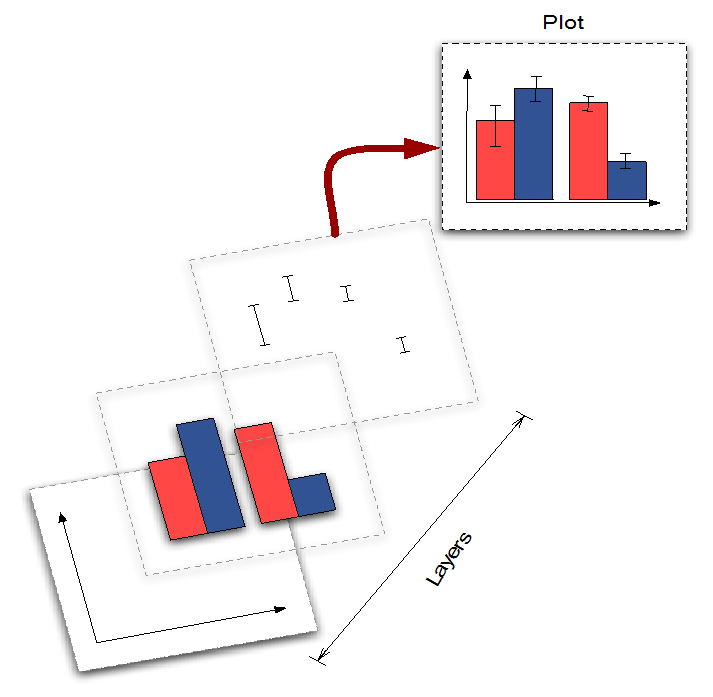
\includegraphics[width=0.30000\textwidth]{Images/08_ggplot_Layers.PNG}
\caption{\textbf{Abbildung 27}: Layers in ggplot}
\end{figure}

Jeder Layer kann für sich gesehen ein bestimmtes Aussehen (aesthetic)
und auch bestimmte geometrische Objekte (Balken, Linien, etc.)
beinhalten.

\begin{figure}
\centering
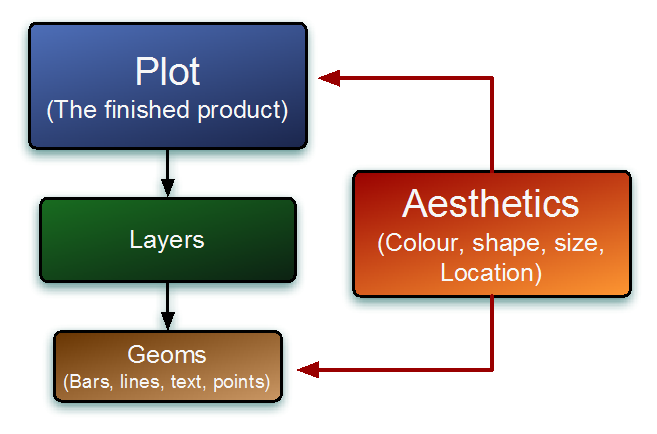
\includegraphics[width=0.30000\textwidth]{Images/08_ggplot_Anatomy.PNG}
\caption{\textbf{Abbildung 28}: Anatomie von ggplot}
\end{figure}

Die Aesthetics (aes()) bestimmen das Aussehen wie z.B. Farbe, Größe,
Positionen, Stile, etc.

\begin{figure}
\centering
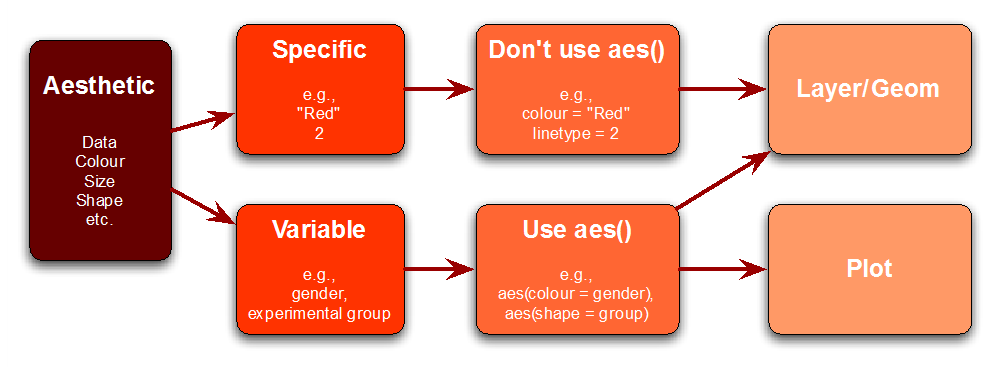
\includegraphics[width=0.30000\textwidth]{Images/08_ggplot_Aesthetics.PNG}
\caption{\textbf{Abbildung 29}: Aesthetics in ggplot}
\end{figure}

Die geometrischen Objekte in einem Plot definieren die Darstellungsform
der Daten. Auszugsweise mögliche geom's von ggplot:

\begin{itemize}
\tightlist
\item
  geom\_bar()
\item
  geom\_point()
\item
  geom\_line()
\item
  geom\_histogram()
\item
  geom\_boxplot()
\end{itemize}

\paragraph{Verwendung von ggplot2}\label{verwendung-von-ggplot2}
\addcontentsline{toc}{paragraph}{Verwendung von ggplot2}

Aufgrund des enormen Leistungsumfangs von ggplot, wollen wir im
folgenden (mit der Topdown-Methode) einen Einblick in die vielseitige
Verwendbarkeit des Pakets durch Beispiele aus
\href{http://www.cookbook-r.com/Graphs/}{Cookbook R} gewinnen. Öffne den
Link und gehe im Kapitel \emph{Graphs with ggplot2} zu den \emph{Bar and
line graphs (ggplot2)}.

Gehen wir einmal davon aus, dass wir für unsere Daten aus
\emph{hyper.sav} ein Balkendiagramm des durchschnittlichen BMI getrennt
nach Altersklasse (x-Achse) und Geschlecht (Balken) erzeugen wollen. Wir
durchsuchen die geöffnete Cookbook-Seite und finden folgende Darstellung
als passend für unsere Daten:

\begin{figure}
\centering
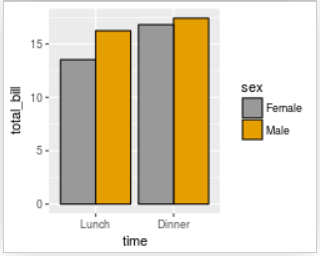
\includegraphics[width=0.30000\textwidth]{Images/08_ggplot_Beispiel1.PNG}
\caption{\textbf{Abbildung 30}: Vorlage für das gewünschte
Balkendiagramm}
\end{figure}

\begin{enumerate}
\def\labelenumi{\arabic{enumi}.}
\tightlist
\item
  Im ersten Schritt kopieren wir den entsprechenden Code in unseren
  Editor und führen diesen aus (\emph{Hinweis}: kopiere auch den Code
  der Website, in dem die Daten definiert werden!).
\item
  Wenn dieser Code auch denselben Output wie auf der Website erzeugt,
  versuchen wir nun durch Änderung der entsprechenden Daten im Code
  diesen Plot an unsere Daten (hyper.sav) anzupassen.
\item
  Nachdem der Graph für unsere Daten adaptiert wurde, speichern wir
  diesen in das Verzeichnis \emph{/images}.
\end{enumerate}

\begin{Shaded}
\begin{Highlighting}[]
\NormalTok{  dat1 <-}\StringTok{ }\KeywordTok{data.frame}\NormalTok{(}
    \DataTypeTok{sex =} \KeywordTok{factor}\NormalTok{(}\KeywordTok{c}\NormalTok{(}\StringTok{"Female"}\NormalTok{,}\StringTok{"Female"}\NormalTok{,}\StringTok{"Male"}\NormalTok{,}\StringTok{"Male"}\NormalTok{)),}
    \DataTypeTok{time =} \KeywordTok{factor}\NormalTok{(}\KeywordTok{c}\NormalTok{(}\StringTok{"Lunch"}\NormalTok{,}\StringTok{"Dinner"}\NormalTok{,}\StringTok{"Lunch"}\NormalTok{,}\StringTok{"Dinner"}\NormalTok{), }\DataTypeTok{levels=}\KeywordTok{c}\NormalTok{(}\StringTok{"Lunch"}\NormalTok{,}\StringTok{"Dinner"}\NormalTok{)),}
    \DataTypeTok{total_bill =} \KeywordTok{c}\NormalTok{(}\FloatTok{13.53}\NormalTok{, }\FloatTok{16.81}\NormalTok{, }\FloatTok{16.24}\NormalTok{, }\FloatTok{17.42}\NormalTok{))}
  
  \KeywordTok{head}\NormalTok{(dat1)}
  
  \KeywordTok{ggplot}\NormalTok{(}\DataTypeTok{data =}\NormalTok{ dat1, }
         \KeywordTok{aes}\NormalTok{(}\DataTypeTok{x =}\NormalTok{ time, }\DataTypeTok{y =}\NormalTok{ total_bill, }\DataTypeTok{fill =}\NormalTok{ sex)) }\OperatorTok{+}
\StringTok{    }\KeywordTok{geom_bar}\NormalTok{(}\DataTypeTok{stat =} \StringTok{"identity"}\NormalTok{, }
             \DataTypeTok{position=}\KeywordTok{position_dodge}\NormalTok{(), }
             \DataTypeTok{colour =} \StringTok{"black"}\NormalTok{) }\OperatorTok{+}
\StringTok{    }\KeywordTok{scale_fill_manual}\NormalTok{(}\DataTypeTok{values=}\KeywordTok{c}\NormalTok{(}\StringTok{"#999999"}\NormalTok{, }\StringTok{"#E69F00"}\NormalTok{))}
\end{Highlighting}
\end{Shaded}

\paragraph{Datenformat in ggplot2}\label{datenformat-in-ggplot2}
\addcontentsline{toc}{paragraph}{Datenformat in ggplot2}

\emph{ggplot2} ist grundsätzlich auf sogenannte ``long format'' Daten
ausgelegt. Um die Repräsentativität von ``wide format'' Datensätzen zu
erhöhen, also Datensätze mit sehr vielen verschiedenen Merkmalen, gibt
es in R die Pakete \emph{reshape2} und \emph{plyr}, die häufig zur
Datenmanipulation\footnote{Datenmanipulation meint hierbei das
  Schichten, Gruppieren und Zusammenfassen verschiedener Daten.}
verwendet werden.

\begin{center}\rule{0.5\linewidth}{\linethickness}\end{center}

\subsection*{Lösungen}\label{losungen-2}
\addcontentsline{toc}{subsection}{Lösungen}

\subsubsection{Lösung Funktion
Standardfehler}\label{losung-funktion-standardfehler}

\begin{Shaded}
\begin{Highlighting}[]
\NormalTok{  SE <-}\StringTok{ }\ControlFlowTok{function}\NormalTok{(x) \{}
\NormalTok{    SE <-}\StringTok{ }\KeywordTok{sd}\NormalTok{(x) }\OperatorTok{/}\StringTok{ }\KeywordTok{length}\NormalTok{(x)}
    \KeywordTok{return}\NormalTok{(SE)}
\NormalTok{  \}}
  \KeywordTok{SE}\NormalTok{(DF}\OperatorTok{$}\NormalTok{alter)}
\end{Highlighting}
\end{Shaded}

\subsubsection{Lösung ggplot Beispiel 1}\label{losung-ggplot-beispiel-1}

\begin{Shaded}
\begin{Highlighting}[]
\NormalTok{  dat1 <-}\StringTok{ }\KeywordTok{summaryBy}\NormalTok{(BMI }\OperatorTok{~}\StringTok{ }\NormalTok{ak }\OperatorTok{+}\StringTok{ }\NormalTok{geschlecht, DF)}
  \KeywordTok{str}\NormalTok{(dat1)}
  \KeywordTok{ggplot}\NormalTok{(}\DataTypeTok{data =}\NormalTok{ dat1, }
         \KeywordTok{aes}\NormalTok{(}\DataTypeTok{x =}\NormalTok{ ak, }\DataTypeTok{y =}\NormalTok{ BMI.mean, }\DataTypeTok{fill =}\NormalTok{ geschlecht)) }\OperatorTok{+}
\StringTok{    }\KeywordTok{geom_bar}\NormalTok{(}\DataTypeTok{stat=}\StringTok{"identity"}\NormalTok{, }
             \DataTypeTok{position=}\KeywordTok{position_dodge}\NormalTok{(), }
             \DataTypeTok{colour=}\StringTok{"black"}\NormalTok{) }\OperatorTok{+}
\StringTok{    }\KeywordTok{scale_fill_manual}\NormalTok{(}\DataTypeTok{values=}\KeywordTok{c}\NormalTok{(}\StringTok{"#999999"}\NormalTok{, }\StringTok{"#E69F00"}\NormalTok{))}
\end{Highlighting}
\end{Shaded}

\section{Datenauswertung Lime Survey}\label{datenauswertung-lime-survey}

Im nachfolgenden Beispiel werden die Daten des World-Knowledge-Test
ausgewertet. Bei diesem Test handelt es sich um eine einfache Umfrage,
welche mit dem Online-Survey-Tool \emph{LimeSurvey} erstellt wurde. Die
Befragung richtete sich an ca. 300 StudentInnen der Universität
Salzburg. Die Daten sollen im Folgenden zur Auswertung einfacher
deskriptiver Statistiken mit R verwendet werden.

\begin{figure}
\centering
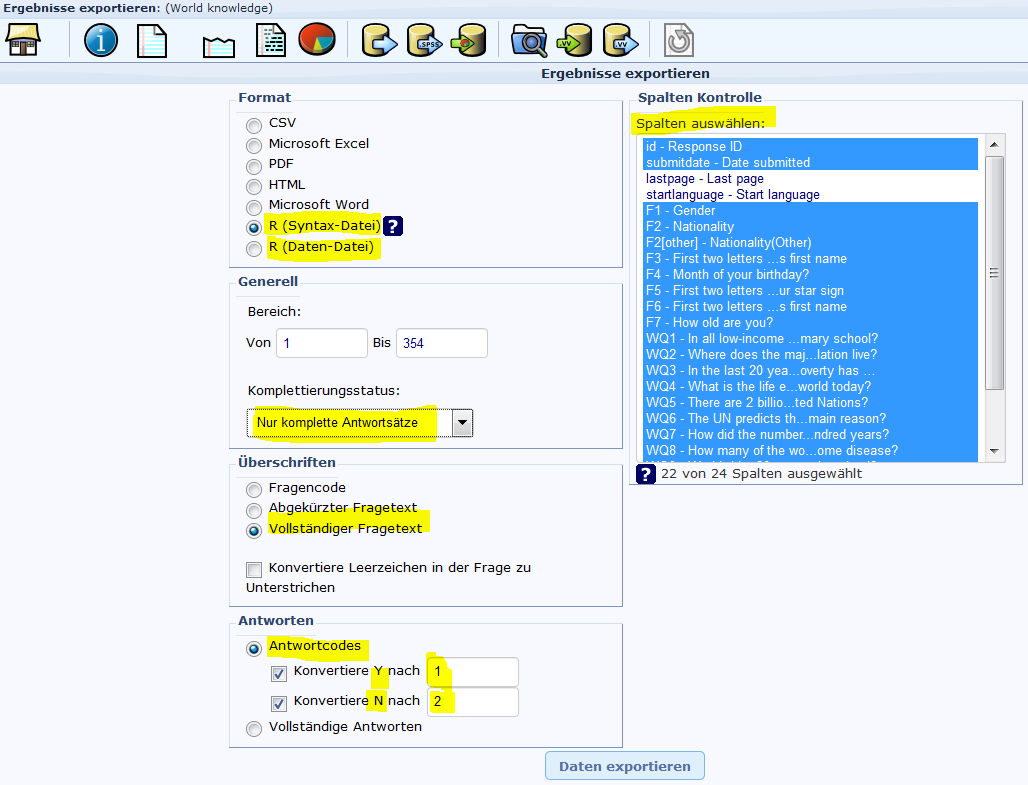
\includegraphics[width=0.70000\textwidth]{Images/09_R_LimeSurveyExport.PNG}
\caption{\textbf{Abbildung 31}: Export der Daten aus Lime Survey}
\end{figure}

LimeSurvey bietet die Möglichkeit, Umfragedaten in verschiedensten
Formaten zu exportieren. Wie in obiger Dartellung ersichtlich, bietet
sich unter anderem der Export einer R-Daten als auch R-Syntax Datei.
Nach Durchführung des Exorts stehen zwei Dateien zur Verfügung:

\begin{figure}
\centering
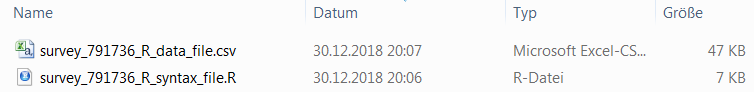
\includegraphics[width=0.70000\textwidth]{Images/09_R_LimeSurveyExportDateien.PNG}
\caption{\textbf{Abbildung 32}: Files die aus Lime Survey exportiert
wurden}
\end{figure}

Nachfolgend ein Auszug aus der R-Syntaxdatei:

\begin{Shaded}
\begin{Highlighting}[]
\NormalTok{data <-}\StringTok{ }\KeywordTok{read.csv}\NormalTok{(}\StringTok{"survey_791736_R_data_file.csv"}\NormalTok{, }
                 \DataTypeTok{quote            =} \StringTok{"'}\CharTok{\textbackslash{}"}\StringTok{"}\NormalTok{, }
                 \DataTypeTok{na.strings       =} \KeywordTok{c}\NormalTok{(}\StringTok{""}\NormalTok{, }\StringTok{"}\CharTok{\textbackslash{}"\textbackslash{}"}\StringTok{"}\NormalTok{), }
                 \DataTypeTok{stringsAsFactors =} \OtherTok{FALSE}\NormalTok{)}

\CommentTok{# LimeSurvey Field type: F}
\NormalTok{  data[, }\DecValTok{1}\NormalTok{] <-}\StringTok{ }\KeywordTok{as.numeric}\NormalTok{(data[, }\DecValTok{1}\NormalTok{])}
  \KeywordTok{attributes}\NormalTok{(data)}\OperatorTok{$}\NormalTok{variable.labels[}\DecValTok{1}\NormalTok{] <-}\StringTok{ "id"}
  \KeywordTok{names}\NormalTok{(data)[}\DecValTok{1}\NormalTok{] <-}\StringTok{ "id"}
\CommentTok{# LimeSurvey Field type: DATETIME23.2}
\NormalTok{  data[, }\DecValTok{2}\NormalTok{] <-}\StringTok{ }\KeywordTok{as.character}\NormalTok{(data[, }\DecValTok{2}\NormalTok{])}
  \KeywordTok{attributes}\NormalTok{(data)}\OperatorTok{$}\NormalTok{variable.labels[}\DecValTok{2}\NormalTok{] <-}\StringTok{ "submitdate"}
  \KeywordTok{names}\NormalTok{(data)[}\DecValTok{2}\NormalTok{] <-}\StringTok{ "submitdate"}
\CommentTok{# LimeSurvey Field type: F}
\NormalTok{  data[, }\DecValTok{3}\NormalTok{] <-}\StringTok{ }\KeywordTok{as.numeric}\NormalTok{(data[, }\DecValTok{3}\NormalTok{])}
  \KeywordTok{attributes}\NormalTok{(data)}\OperatorTok{$}\NormalTok{variable.labels[}\DecValTok{3}\NormalTok{] <-}\StringTok{ "Gender"}
\NormalTok{  data[, }\DecValTok{3}\NormalTok{] <-}\StringTok{ }\KeywordTok{factor}\NormalTok{(data[, }\DecValTok{3}\NormalTok{], }\DataTypeTok{levels=}\KeywordTok{c}\NormalTok{(}\DecValTok{1}\NormalTok{,}\DecValTok{2}\NormalTok{),}\DataTypeTok{labels=}\KeywordTok{c}\NormalTok{(}\StringTok{"weiblich"}\NormalTok{, }\StringTok{"männlich"}\NormalTok{))}
  \KeywordTok{names}\NormalTok{(data)[}\DecValTok{3}\NormalTok{] <-}\StringTok{ "F1"}
\CommentTok{# LimeSurvey Field type: A}
\NormalTok{  ...}
\end{Highlighting}
\end{Shaded}

Nach dem Laden der Datendatei (\emph{survey\_791736\_R\_data\_file.csv})
werden Formatierungen der Datentypen und Vergabe von Variablennamen
durchgeführt. Da Variablennamen von LimeSurvey vergeben werden, ist es
in den meisten Fällen sinnvoll, diese manuell zu ändern. Auch eine
genaue Kontrolle (und gegebenenfalls Korrektur) bei den Datentypen ist
angebracht.

Üblicherweise ändert sich eine Umfrage nach Freischaltung bezüglich
ihrer Datenstruktur nicht mehr, daher ist dieser Aufwand auch nur
einmalig durchzuführen. \emph{WICHTIG}: bei allen folgenden Exports aus
Limesurvey ist dann nur mehr die Datendatei zu exportieren - die
Syntaxdatei braucht dann nicht mehr exportiert werden\footnote{es sei
  denn, die Struktur der Umfrage ändert sich wider erwarten!}!

\subsection*{Datenvorverarbeitung}\label{datenvorverarbeitung}
\addcontentsline{toc}{subsection}{Datenvorverarbeitung}

Lade und überarbeite die Syntaxdatei
(\emph{survey\_791736\_R\_syntax\_file.R}). Beachte dabei folgende
Punkte:

\begin{itemize}
\tightlist
\item
  Sonderzeichen werden oft nicht korrekt übernommen - verwende die
  RStudio-Funktion Search and Replace um alle falsch übertragenen
  Sonderzeichen zu korrigieren.
\item
  Ändere die Variablennamen auf \emph{sinnvolle} Namen (vgl. Attribute)
\item
  Überprüfe die Datentypen sämtlicher Variablen. Ändere den Datentyp der
  Variablen falls notwendig.
\end{itemize}

Nach erfolgter Überarbeitung kann das Skript in eine Funktion
umgewandelt werden. Der Name der Funktion sollte dabei
\emph{LS\_Import.R} lauten und als einziges Argument sollte die Variable
\emph{F2L} (für File t(w)o Load) angegeben werden.

\emph{Hinweis:} die Funktion \emph{read.csv()} muss entsprechend
angepasst werden!

\begin{Shaded}
\begin{Highlighting}[]
\NormalTok{LS_Import <-}\StringTok{ }\ControlFlowTok{function}\NormalTok{(F2L) \{}
\NormalTok{  data <-}\StringTok{ }\KeywordTok{read.csv}\NormalTok{(F2L,}
                   \DataTypeTok{quote            =} \StringTok{"'}\CharTok{\textbackslash{}"}\StringTok{"}\NormalTok{,}
                   \DataTypeTok{na.strings       =} \KeywordTok{c}\NormalTok{(}\StringTok{""}\NormalTok{, }\StringTok{"}\CharTok{\textbackslash{}"\textbackslash{}"}\StringTok{"}\NormalTok{),}
                   \DataTypeTok{stringsAsFactors =} \OtherTok{FALSE}\NormalTok{)}
  
  \CommentTok{# LimeSurvey Field type: F}
\NormalTok{  data[, }\DecValTok{1}\NormalTok{] <-}\StringTok{ }\KeywordTok{as.numeric}\NormalTok{(data[, }\DecValTok{1}\NormalTok{])}
  \KeywordTok{attributes}\NormalTok{(data)}\OperatorTok{$}\NormalTok{variable.labels[}\DecValTok{1}\NormalTok{] <-}\StringTok{ "id"}
  \KeywordTok{names}\NormalTok{(data)[}\DecValTok{1}\NormalTok{] <-}\StringTok{ "id"}
  \CommentTok{# LimeSurvey Field type: DATETIME23.2}
\NormalTok{  ...}
\end{Highlighting}
\end{Shaded}

Des Weiteren sollte am Ende der Funktion als Rückgabewert der Datenframe
(data) angegeben werden (siehe nachfolgenden Codteil am Ende der
\emph{LS\_Import.R} Funktion):

\begin{Shaded}
\begin{Highlighting}[]
\NormalTok{  ...}
  \KeywordTok{names}\NormalTok{(data)[}\DecValTok{22}\NormalTok{] <-}\StringTok{ "WQ12"}
  
  \KeywordTok{return}\NormalTok{(data)}
\ErrorTok{\}}
\end{Highlighting}
\end{Shaded}

\subsubsection*{Aufgabe 1}\label{aufgabe-1-1}
\addcontentsline{toc}{subsubsection}{Aufgabe 1}

Erstelle nun ein neues Skript (Name: \emph{09\_RLimeSurvey.R}), in
welchen du zuerst den Standard-Header kopierst (siehe nachfolgenden
Code) und welches danach die Daten über die soeben erstellte Funktion
lädt! Prüfe mit einer geeigneten Funktion die Struktur des geladenen
Dataframes.

\begin{Shaded}
\begin{Highlighting}[]
\CommentTok{#---- 09_RLS_Init}
  \KeywordTok{rm}\NormalTok{(}\DataTypeTok{list =} \KeywordTok{ls}\NormalTok{())}
  \ControlFlowTok{if}\NormalTok{ (}\OperatorTok{!}\KeywordTok{require}\NormalTok{(}\StringTok{"pacman"}\NormalTok{)) }\KeywordTok{install.packages}\NormalTok{(}\StringTok{"pacman"}\NormalTok{)}
\NormalTok{  pacman}\OperatorTok{::}\KeywordTok{p_load}\NormalTok{(here)}
\end{Highlighting}
\end{Shaded}

Durch diese Funktion können die Daten fortlaufend auf dem aktuellen
Stand gehalten werden. Der einzige Nachteil besteht noch darin, dass man
manuell die Daten aus LimeSurvey exportieren muss. Dass kann allerdings
automatisiert werden. Dazu braucht man nur den Zugang zur SQL-Datenbank
von Limesurvey und die entsprechenden Pakete in R laden. Aus
Datenschutzgründen ist es im Rahmen dieser LV nicht möglich, den Zugang
zur LS-Datenbank freizuschalten, daher werden wir diese Möglichkeit
nicht weiter besprechen. Es sei jedoch an dieser Stelle darauf
hingewiesen, dass man mit einem entsprechenden Zugang zu den Daten auch
die Möglichkeit hat, Skripte und Funktionen in R in die Aufgabenplanung
eines Windows/Linux-Systems einzubauen (sogenannte chron-jobs) und damit
ein vollständig automatisches Auswertesystem zu erstellen.

\subsection*{Deskriptive Statistik}\label{deskriptive-statistik}
\addcontentsline{toc}{subsection}{Deskriptive Statistik}

Bei den nachfolgenden Aufgaben erzeugen wir deskriptive Statistiken in
Form von Tabellen und einer Graphik.

\hypertarget{aufgabe-2}{\subsubsection*{Aufgabe 2}\label{aufgabe-2}}
\addcontentsline{toc}{subsubsection}{Aufgabe 2}

Im Folgendem wollen wir und mit der einfachen Auswertung der
vorliegenden Daten beschäftigen. Die ersten Schritte einer
Datenauswertung beginnen i.A. mit einer deskriptiven Statistik. Aufgrund
der vorwiegend nominalen Daten des Fragebogens eignen sich am besten
Häufigkeitstabellen. Erstelle daher folgende Tabellen (verwende dazu die
Funktion \emph{table()}):

\begin{enumerate}
\def\labelenumi{\arabic{enumi}.}
\tightlist
\item
  Anzahl der Männer und Frauen die an der Umfrage teilgenommen haben.
\item
  Anzahl der Personen je Nation.
\item
  Anzahl der Personen nur jener Nationen, die an der Umfrage
  teilgenommen haben\footnote{\emph{Hinweis:} verwende die Funktion
    \emph{droplevels()}}.
\item
  Anzahl der Personen nur jener Nationen, die an der Umfrage
  teilgenommen haben, getrennt nach Geschlecht.
\item
  Gleich wie Aufgabe 4, nur mit zusätzlicher Angabe der Randsummen!
\item
  Gleich wie Aufgabe 5, nur die auf 2 Stellen gerundeten Angaben in
  Prozent\footnote{\emph{Hinweis:} runden mit der Funktion
    \emph{round()}, Prozente mit der Funktion \emph{prop.table()}}.
\end{enumerate}

\subsubsection*{Aufgabe 3}\label{aufgabe-3}
\addcontentsline{toc}{subsubsection}{Aufgabe 3}

Ein zur deskriptiven Analyse hilfreiches Paket ist \emph{doBy}. Wir
wollen die darin enthaltene Funktion \emph{summaryBy()} verwenden, um
folgende Aufgabenstellungen zu lösen:

\begin{enumerate}
\def\labelenumi{\arabic{enumi}.}
\tightlist
\item
  Berechne das Durchschnittsalter getrennt nach Geschlecht.
\item
  Berechne den Mittelwert, die Standardabweichung, die Varianz, das
  Minimum und das Maximum der Variablen Alter getrennt nach Geschlecht.
\item
  Berechne das Durchschnittsalter getrennt nach Geschlecht und
  Nationalität.
\item
  Berechne den Mittelwert, die Standardabweichung, die Varianz, das
  Minimum und das Maximum der Variablen Alter getrennt nach Geschlecht
  und Nationalität.
\end{enumerate}

Das Paket doBy bietet darüber hinaus eine Vielzahl von Funktionen, die
vor allem für das Arbeiten mit gruppierten Daten sehr hilfreich sein
können. Hingewiesen sei noch auf die Möglichkeit der Berechnung von
Kontrasten im Rahmen einer \emph{least square mean} (ANOVA) Analyse. Es
würde den Rahmen dieser LV sprengen, alle verfügbaren Funktionen zu
besprechen und zu verwenden. Weitere Details zu diesem Paket sind der
\href{https://cran.r-project.org/web/packages/doBy/doBy.pdf}{Dokumentation}
zu entnehmen.

\subsubsection*{Aufgabe 4}\label{aufgabe-4}
\addcontentsline{toc}{subsubsection}{Aufgabe 4}

Neben den Tabellen spielen Graphiken eine wesentliche Rolle in der
deskriptiven Statistik. In dieser Aufgabe wollen wir mit dem Paket
\emph{ggplot2} ein Balkendiagramm erstellen, welche für die erste Frage
des Tests die prozentuellen Anteile pro Antwortkategorie getrennt nach
Geschlecht darstellt. Darüber hinaus sollte in dieser Graphik auch
jeweils ein Balken pro Antwortkategorie für den prozentuellen Anteil
unabhängig vom Geschlecht angezeigt werden. Folgende Graphik stellt das
gewünschte Ergebnis dar:

\begin{figure}
\centering
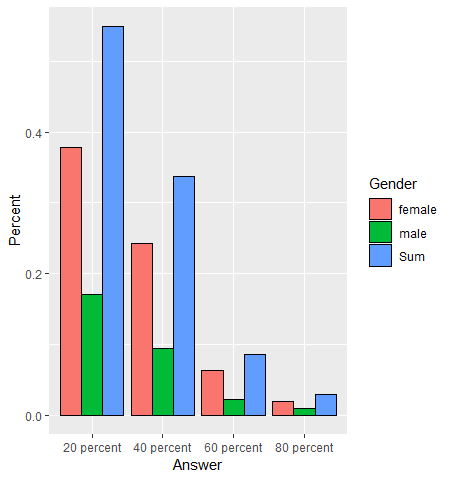
\includegraphics[width=0.40000\textwidth]{Images/09_Aufgabe4_Graphik.PNG}
\caption{\textbf{Abbildung 33}: Vorlage für die Graphik der Aufgabe 4}
\end{figure}

Um die Aufgabe auf das eigentliche Ziel (eine Graphik zu erstellen) zu
beschränken, kannst du den folgenden Code in dein R-Skript kopieren
(diskutiere das Ergebnis dieses Codefragmentes)\footnote{die Definition
  von \emph{LegTit} und \emph{WQ\_Label} wird in einer Folgeaufgabe noch
  zur weiteren Gestaltung der Graphik verwendet.}:

\begin{Shaded}
\begin{Highlighting}[]
  \KeywordTok{library}\NormalTok{(ggplot2)}
  
\NormalTok{  LegTit          <-}\StringTok{ }\KeywordTok{paste0}\NormalTok{(}\StringTok{'Overall (N  =  '}\NormalTok{, }\KeywordTok{dim}\NormalTok{(DF)[}\DecValTok{1}\NormalTok{], }\StringTok{') answers in %'}\NormalTok{)  }
\NormalTok{  ColInd          <-}\StringTok{ }\KeywordTok{which}\NormalTok{(}\KeywordTok{colnames}\NormalTok{(DF) }\OperatorTok\StringTok{ }\KeywordTok{c}\NormalTok{(}\StringTok{"WQ1"}\NormalTok{))}
\NormalTok{  WQ_Label        <-}\StringTok{ }\KeywordTok{attributes}\NormalTok{(DF)}\OperatorTok{$}\NormalTok{variable.labels[ColInd]}

\NormalTok{  CT              <-}\StringTok{ }\KeywordTok{round}\NormalTok{(}\DecValTok{100}\OperatorTok{*}\KeywordTok{addmargins}\NormalTok{(}\KeywordTok{prop.table}\NormalTok{(}\KeywordTok{table}\NormalTok{(DF[,ColInd], DF}\OperatorTok{$}\NormalTok{Gender)), }
                                          \DataTypeTok{margin  =}  \DecValTok{2}\NormalTok{), }\DecValTok{2}\NormalTok{)}
\NormalTok{  DF_CT           <-}\StringTok{ }\KeywordTok{as.data.frame}\NormalTok{(CT)}
  \KeywordTok{colnames}\NormalTok{(DF_CT) <-}\StringTok{ }\KeywordTok{c}\NormalTok{(}\StringTok{"Answer"}\NormalTok{, }\StringTok{"Gender"}\NormalTok{, }\StringTok{"Percent"}\NormalTok{)}
\end{Highlighting}
\end{Shaded}

Ergänze nun den Code mit der entsprechenden Funktion zur Erstellung
dieser Graphik und ergänze/ändere den Graphen nach folgenden Vorgaben:

\begin{enumerate}
\def\labelenumi{\arabic{enumi}.}
\tightlist
\item
  Drehe die Koordinaten 90 Grad (verwende die Funktion
  \emph{coord\_flip()}).
\item
  Die x-Achsenbeschriftung sollte \emph{Answer} sein (verwende die
  Funktion \emph{xlab()}).
\item
  Die Beschriftung der Legende sollte dem bereits definierten Text der
  Variablen \emph{LegTit} entsprechen (verwende die Funktion
  \emph{guides(fill = guide\_legend(title = ???))}).
\item
  Verwende die Funktion \emph{labs()}, um Titel (= \emph{WQ\_Label}),
  Subtitel (= \emph{``World Knowledge Test''}), Caption (=
  \emph{``Source: World Knowledge Query PLUS (2018)''}, tag (=
  \emph{``A''}) anzuzeigen.
\item
  Ändere das Farbschema des Graphen auf Grauschattierungen (verwende die
  Funktion \emph{scale\_fill\_grey()}).
\item
  Zeige über den Balken die jeweilig erreichten Prozentwerte an
  (verwende die Funktion \emph{geom\_text(aes(label = paste0(round(???,
  1), ``\%'')), position = position\_dodge(width=0.9), hjust = -0.25)}).
\item
  Ändere den Hintergrund der Graphik auf Transparent (verwende die
  Funktion \emph{theme\_bw()}).
\end{enumerate}

Der fertige Graph sollte folgendermaßen aussehen:

\begin{figure}
\centering
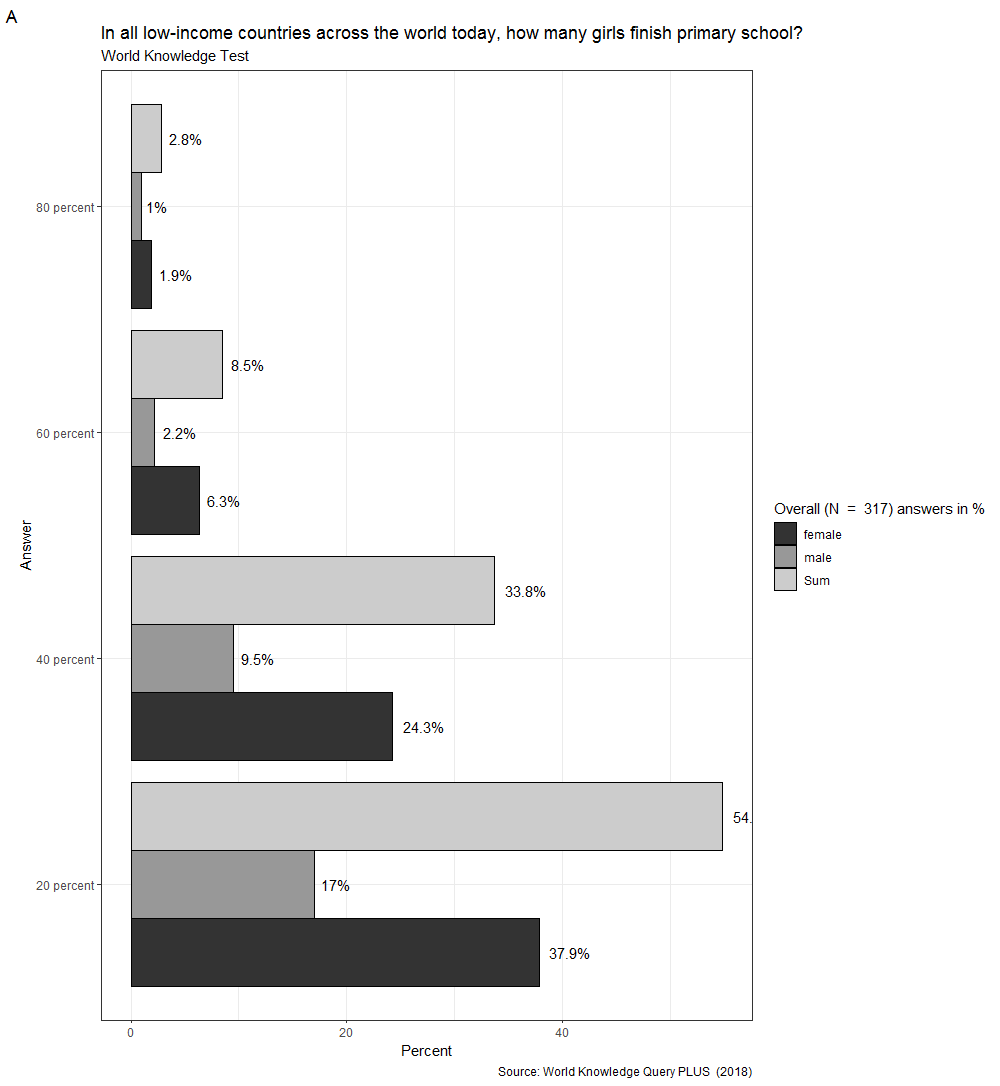
\includegraphics[width=0.60000\textwidth]{Images/09_Aufgabe4_Graphik_Endversion.PNG}
\caption{\textbf{Abbildung 34}: Endversion der Graphik von Aufgabe 4}
\end{figure}

\subsection*{Lösungen}\label{losungen-3}
\addcontentsline{toc}{subsection}{Lösungen}

\subsubsection*{Lösung Aufgabe 1}\label{losung-aufgabe-1}
\addcontentsline{toc}{subsubsection}{Lösung Aufgabe 1}

\begin{Shaded}
\begin{Highlighting}[]
  \KeywordTok{source}\NormalTok{(}\StringTok{"RScripts/LS_Import.R"}\NormalTok{)}
\NormalTok{  F2L <-}\StringTok{ "Data/survey_791736_R_data_file.csv"}
\NormalTok{  DF  <-}\StringTok{ }\KeywordTok{LS_Import}\NormalTok{(}\DataTypeTok{F2L =}\NormalTok{ F2L)}
  \KeywordTok{str}\NormalTok{(DF)}
\end{Highlighting}
\end{Shaded}

\subsubsection*{Lösung Aufgabe 2}\label{losung-aufgabe-2}
\addcontentsline{toc}{subsubsection}{Lösung Aufgabe 2}

\begin{Shaded}
\begin{Highlighting}[]
  \KeywordTok{table}\NormalTok{(DF}\OperatorTok{$}\NormalTok{Gender) }\CommentTok{# A2-1}
  \KeywordTok{table}\NormalTok{(DF}\OperatorTok{$}\NormalTok{Nationality) }\CommentTok{# A2-2}
  \KeywordTok{table}\NormalTok{(}\KeywordTok{droplevels}\NormalTok{(DF}\OperatorTok{$}\NormalTok{Nationality))  }\CommentTok{# A2-3}
  \KeywordTok{table}\NormalTok{(DF}\OperatorTok{$}\NormalTok{Gender, }\KeywordTok{droplevels}\NormalTok{(DF}\OperatorTok{$}\NormalTok{Nationality)) }\CommentTok{# A2-4}
  \KeywordTok{addmargins}\NormalTok{(}\KeywordTok{table}\NormalTok{(DF}\OperatorTok{$}\NormalTok{Gender, }\KeywordTok{droplevels}\NormalTok{(DF}\OperatorTok{$}\NormalTok{Nationality))) }\CommentTok{# A2-5}
  \KeywordTok{addmargins}\NormalTok{(}\KeywordTok{round}\NormalTok{(}\KeywordTok{prop.table}\NormalTok{(}\KeywordTok{table}\NormalTok{(DF}\OperatorTok{$}\NormalTok{Gender, }\KeywordTok{droplevels}\NormalTok{(DF}\OperatorTok{$}\NormalTok{Nationality)))}\OperatorTok{*}\DecValTok{100}\NormalTok{,}\DecValTok{2}\NormalTok{)) }\CommentTok{# A2-6}
\end{Highlighting}
\end{Shaded}

\subsubsection*{Lösung Aufgabe 3}\label{losung-aufgabe-3}
\addcontentsline{toc}{subsubsection}{Lösung Aufgabe 3}

\begin{Shaded}
\begin{Highlighting}[]
  \KeywordTok{library}\NormalTok{(doBy)}
  \KeywordTok{summaryBy}\NormalTok{(}\DataTypeTok{formula =}\NormalTok{ Age }\OperatorTok{~}\StringTok{ }\NormalTok{Gender, }
            \DataTypeTok{data    =}\NormalTok{ DF) }\CommentTok{# A3-1}
  \KeywordTok{summaryBy}\NormalTok{(}\DataTypeTok{formula =}\NormalTok{ Age }\OperatorTok{~}\StringTok{ }\NormalTok{Gender, }
            \DataTypeTok{data    =}\NormalTok{ DF, }
            \DataTypeTok{FUN     =} \KeywordTok{c}\NormalTok{(mean, sd, var, min, max)) }\CommentTok{# A3-2}
  \KeywordTok{summaryBy}\NormalTok{(}\DataTypeTok{formula =}\NormalTok{ Age }\OperatorTok{~}\StringTok{ }\NormalTok{Gender }\OperatorTok{+}\StringTok{ }\NormalTok{Nationality, }
            \DataTypeTok{data    =}\NormalTok{ DF) }\CommentTok{# A3-3}
  \KeywordTok{summaryBy}\NormalTok{(}\DataTypeTok{formula =}\NormalTok{ Age }\OperatorTok{~}\StringTok{ }\NormalTok{Gender }\OperatorTok{+}\StringTok{ }\NormalTok{Nationality, }
            \DataTypeTok{data    =}\NormalTok{ DF, }
            \DataTypeTok{FUN     =} \KeywordTok{c}\NormalTok{(mean, sd, var)) }\CommentTok{# A3-4}
\end{Highlighting}
\end{Shaded}

\subsubsection*{Lösung Aufgabe 4}\label{losung-aufgabe-4}
\addcontentsline{toc}{subsubsection}{Lösung Aufgabe 4}

\begin{Shaded}
\begin{Highlighting}[]
  \KeywordTok{library}\NormalTok{(ggplot2)}
  
\NormalTok{  LegTit          <-}\StringTok{ }\KeywordTok{paste0}\NormalTok{(}\StringTok{'Overall (N  =  '}\NormalTok{, }\KeywordTok{dim}\NormalTok{(DF)[}\DecValTok{1}\NormalTok{], }\StringTok{') answers in %'}\NormalTok{)  }
\NormalTok{  ColInd          <-}\StringTok{ }\KeywordTok{which}\NormalTok{(}\KeywordTok{colnames}\NormalTok{(DF) }\OperatorTok\StringTok{ }\KeywordTok{c}\NormalTok{(}\StringTok{"WQ1"}\NormalTok{))}
\NormalTok{  WQ_Label        <-}\StringTok{ }\KeywordTok{attributes}\NormalTok{(DF)}\OperatorTok{$}\NormalTok{variable.labels[ColInd]}

\NormalTok{  CT              <-}\StringTok{ }\KeywordTok{round}\NormalTok{(}\DecValTok{100}\OperatorTok{*}\KeywordTok{addmargins}\NormalTok{(}\KeywordTok{prop.table}\NormalTok{(}\KeywordTok{table}\NormalTok{(DF[,ColInd], DF}\OperatorTok{$}\NormalTok{Gender)), }\DataTypeTok{margin  =}  \DecValTok{2}\NormalTok{), }\DecValTok{2}\NormalTok{)}
\NormalTok{  DF_CT           <-}\StringTok{ }\KeywordTok{as.data.frame}\NormalTok{(CT)}
  \KeywordTok{colnames}\NormalTok{(DF_CT) <-}\StringTok{ }\KeywordTok{c}\NormalTok{(}\StringTok{"Answer"}\NormalTok{, }\StringTok{"Gender"}\NormalTok{, }\StringTok{"Percent"}\NormalTok{)}
  
  \KeywordTok{ggplot}\NormalTok{(DF_CT, }\KeywordTok{aes}\NormalTok{(}\DataTypeTok{x  =}\NormalTok{  Answer, }\DataTypeTok{y  =}\NormalTok{  Percent, }\DataTypeTok{fill  =}\NormalTok{  Gender)) }\OperatorTok{+}
\StringTok{        }\KeywordTok{geom_bar}\NormalTok{(}\DataTypeTok{position =} \KeywordTok{position_dodge}\NormalTok{(), }\DataTypeTok{stat =} \StringTok{"identity"}\NormalTok{,}
                 \DataTypeTok{colour =} \StringTok{"black"}\NormalTok{, }\CommentTok{# Use black outlines,}
                 \DataTypeTok{size =}\NormalTok{ .}\DecValTok{3}\NormalTok{) }\OperatorTok{+}
\StringTok{    }\KeywordTok{coord_flip}\NormalTok{() }\OperatorTok{+}
\StringTok{    }\KeywordTok{xlab}\NormalTok{(}\StringTok{"Answer"}\NormalTok{) }\OperatorTok{+}
\StringTok{    }\KeywordTok{guides}\NormalTok{(}\DataTypeTok{fill =} \KeywordTok{guide_legend}\NormalTok{(}\DataTypeTok{title =}\NormalTok{ LegTit)) }\OperatorTok{+}
\StringTok{    }\KeywordTok{labs}\NormalTok{(}\DataTypeTok{title    =}\NormalTok{ WQ_Label,}
         \DataTypeTok{subtitle =} \StringTok{"World Knowledge Test"}\NormalTok{,}
         \DataTypeTok{caption  =} \StringTok{"Source: World Knowledge Query PLUS  (2018)"}\NormalTok{,}
         \DataTypeTok{tag      =} \StringTok{"A"}\NormalTok{) }\OperatorTok{+}
\StringTok{    }\KeywordTok{scale_fill_grey}\NormalTok{() }\OperatorTok{+}
\StringTok{    }\KeywordTok{geom_text}\NormalTok{(}\KeywordTok{aes}\NormalTok{(}\DataTypeTok{label =} \KeywordTok{paste0}\NormalTok{(}\KeywordTok{round}\NormalTok{(Percent, }\DecValTok{1}\NormalTok{), }\StringTok{"%"}\NormalTok{)), }
              \DataTypeTok{position  =} \KeywordTok{position_dodge}\NormalTok{(}\DataTypeTok{width=}\FloatTok{0.9}\NormalTok{),}
              \DataTypeTok{hjust     =} \OperatorTok{-}\FloatTok{0.25}\NormalTok{) }\OperatorTok{+}
\StringTok{    }\KeywordTok{theme_bw}\NormalTok{()}
\end{Highlighting}
\end{Shaded}

\section{Bedingungen und Schleifen}\label{bedingungen-und-schleifen}

\subsection*{Bedingte Ausführung}\label{bedingte-ausfuhrung}
\addcontentsline{toc}{subsection}{Bedingte Ausführung}

Normalerweise wird ein R-Code Zeile für Zeile, von oben nach unten,
ausgeführt. Manchmal möchte man aber eine Zeile - oder einen ganzen
Block von Zeilen - nur unter einer bestimmten Bedingung durchführen.
Dazu bietet sich in R die If-Anweisung an.

\subsubsection*{Einfache If-Bedingung}\label{einfache-if-bedingung}
\addcontentsline{toc}{subsubsection}{Einfache If-Bedingung}

Folgende Abbildung zeigt die Programmlogik für eine einfache
If-Bedingung:

\begin{figure}
\centering
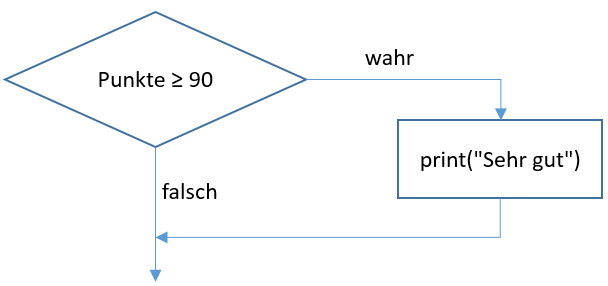
\includegraphics[width=0.50000\textwidth]{Images/10_R_Simple_If.PNG}
\caption{\textbf{Abbildung 35}: Einfaches If}
\end{figure}

Mit folgendem Code kann diese einfache Entscheidung umgesetzt werden:

\begin{Shaded}
\begin{Highlighting}[]
\NormalTok{  punkte <-}\StringTok{ }\DecValTok{90}
  \ControlFlowTok{if}\NormalTok{ (punkte }\OperatorTok{>=}\StringTok{ }\DecValTok{90}\NormalTok{) \{}
    \KeywordTok{print}\NormalTok{(}\StringTok{"Sehr gut"}\NormalTok{)}
\NormalTok{    \}}
\end{Highlighting}
\end{Shaded}

\subsubsection*{Else-If-Bedingung}\label{else-if-bedingung}
\addcontentsline{toc}{subsubsection}{Else-If-Bedingung}

Trifft eine Bedinung nicht zu, kann mit Hilfe der Else-If-Bedingung eine
weitere Bedingung überprüft werden:

\begin{figure}
\centering
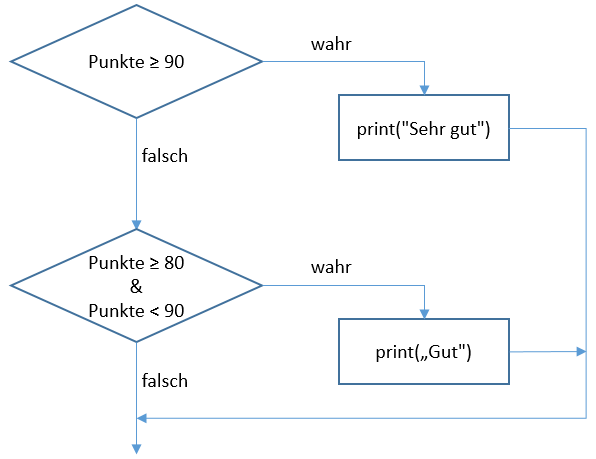
\includegraphics[width=0.50000\textwidth]{Images/10_R_Simple_If_Else.PNG}
\caption{\textbf{Abbildung 36}: Die If-Else Bedingung}
\end{figure}

Folgender Code zeigt die Syntax, mit der eine derartige Überprüfung in R
umgesetzt werden kann:

\begin{Shaded}
\begin{Highlighting}[]
\NormalTok{  punkte <-}\StringTok{ }\DecValTok{85}
  \ControlFlowTok{if}\NormalTok{ (punkte }\OperatorTok{>=}\StringTok{ }\DecValTok{90}\NormalTok{) \{}
    \KeywordTok{print}\NormalTok{(}\StringTok{"Sehr gut"}\NormalTok{)}
\NormalTok{    \} }\ControlFlowTok{else} \ControlFlowTok{if}\NormalTok{ (punkte }\OperatorTok{>=}\StringTok{ }\DecValTok{80} \OperatorTok{&}\StringTok{ }\NormalTok{punkte }\OperatorTok{<}\StringTok{ }\DecValTok{90}\NormalTok{) \{}
    \KeywordTok{print}\NormalTok{(}\StringTok{"Gut"}\NormalTok{);    }
\NormalTok{    \} }\ControlFlowTok{else}\NormalTok{ \{}
      \KeywordTok{print}\NormalTok{(}\StringTok{"Nicht genügend"}\NormalTok{);    }
\NormalTok{  \}}
\end{Highlighting}
\end{Shaded}

\emph{Bemerkung:} bei genauer Betrachtung des Codes kann man
feststellen, dass neben der \emph{if ()} und der \emph{else if ()} auch
eine generelle \emph{else ()} Anweisung am Ende der Entscheidungslogik
verwendet werden kann (aber nicht unbedingt muss). Diese Logik lässt
sich nun für weitere Abfragen erweitern.

\subsubsection*{Aufgabe 1}\label{aufgabe-1-2}
\addcontentsline{toc}{subsubsection}{Aufgabe 1}

Erweitere den Code, sodass für eine beliebige Eingabe von \emph{Punkte}
zwischen 0 und 100 folgende Ausgabe erzeugt wird:

\begin{itemize}
\tightlist
\item
  \(>= 90 \rightarrow\) Sehr gut
\item
  \(>= 80 \& < 90 \rightarrow\) Gut
\item
  \(>= 70 \& < 80 \rightarrow\) Befriedigend
\item
  \(>= 60 \& < 70 \rightarrow\) Genügend
\item
  \(< 60 \rightarrow\) Nicht genügend
\end{itemize}

\protect\hyperlink{aufgabe-1-lsg}{Hier findest du die Lösung zur
Aufgabe}.

\subsubsection*{Die ifelse Bedingung}\label{die-ifelse-bedingung}
\addcontentsline{toc}{subsubsection}{Die ifelse Bedingung}

Eine weitere Möglichkeit bietet noch die folgende
\emph{ifelse(test\_expression, x, y)} Funktion. Betrachte folgendes
Beispiel:

\begin{Shaded}
\begin{Highlighting}[]
\NormalTok{  punkte <-}\StringTok{ }\KeywordTok{sample}\NormalTok{(}\DecValTok{1}\OperatorTok{:}\DecValTok{100}\NormalTok{, }\DecValTok{10}\NormalTok{)}
  \KeywordTok{ifelse}\NormalTok{(punkte }\OperatorTok{<}\StringTok{ }\DecValTok{60}\NormalTok{, }\StringTok{"Nicht genügend"}\NormalTok{, }\StringTok{"Bestanden"}\NormalTok{)}
\end{Highlighting}
\end{Shaded}

\subsection*{Iterationen in R}\label{iterationen-in-r}
\addcontentsline{toc}{subsection}{Iterationen in R}

Sinn und Zweck von Iterationen (\emph{Schleifen}, \emph{Loops}) ist es,
einen Code \(n\)-mal auszuführen. Die Variable \(n\) ist hierbei eine
ganze Zahl (integer) und in der Regel beim Start der Schleife mit einem
festen Wert definiert. In R stehen folgende Loop-Strukturen zur
Verfügung:

\begin{figure}
\centering
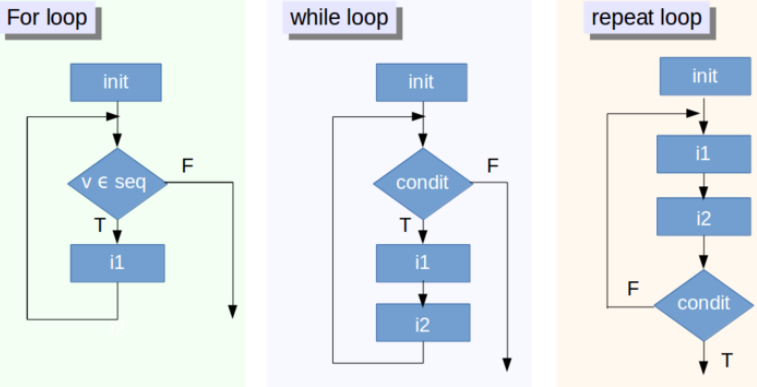
\includegraphics[width=0.70000\textwidth]{Images/10_R_Loops.PNG}
\caption{\textbf{Abbildung 37}: Loop-Strukturen in R}
\end{figure}

Diese Schleifen unterscheiden sich dahingehend:

\begin{itemize}
\tightlist
\item
  \emph{For-Loop}: führt eine Instruktion (\(i1\), \(i2\), etc.) so oft
  durch, bis das Ende einer vordefinierten Sequenz (z.B. 1:100) erreicht
  ist.
\item
  \emph{While-Loop}: so lange eine Bedingung zutrifft (wahr ist), werden
  die Instruktionen \(i1\), \(i2\), etc. ausgeführt. Der while-loop wird
  dann beendet, wenn die Bedingung von \emph{wahr} auf \emph{falsch}
  wechselt.
\item
  \emph{Repeat-Loop}: ähnlich dem while, nur dass die Instruktion \(i1\)
  und \(i2\) zumindest einmal ausgführt werden und zwar unabhängig
  davon, was die Bedingung am Ende der Schleife ergibt.
\end{itemize}

\subsubsection*{Die for-Schleife}\label{die-for-schleife}
\addcontentsline{toc}{subsubsection}{Die for-Schleife}

Die Syntax einer \emph{for}-Schleife ist relativ simple:

\begin{Shaded}
\begin{Highlighting}[]
\NormalTok{  n <-}\StringTok{ }\DecValTok{5}
  \ControlFlowTok{for}\NormalTok{(i }\ControlFlowTok{in} \DecValTok{0}\OperatorTok{:}\NormalTok{n) \{}
    \KeywordTok{print}\NormalTok{(i);}
\NormalTok{  \}}
\end{Highlighting}
\end{Shaded}

Manchmal kann es erforderlich sein, eine bestimmte Iteration zu
unterbrechen und zum nächsten Durchlauf weiterzugehen. Dies kann man mit
dem \emph{next}-Befehl erreichen, wie folgender Code zeigt:

\begin{Shaded}
\begin{Highlighting}[]
\NormalTok{  m <-}\StringTok{ }\DecValTok{20}
  \ControlFlowTok{for}\NormalTok{ (k }\ControlFlowTok{in} \DecValTok{1}\OperatorTok{:}\NormalTok{m)\{}
    \ControlFlowTok{if}\NormalTok{ (}\OperatorTok{!}\NormalTok{k }\OperatorTok\StringTok{ }\DecValTok{2}\NormalTok{)}
      \ControlFlowTok{next}
    \KeywordTok{print}\NormalTok{(k)}
\NormalTok{  \}  }
\end{Highlighting}
\end{Shaded}

Eine einfache Anwendung einer for-Schleife wird im nachfolgenden Code
demonstriert. Um eine For-Schleife vorzeitig zu beenden - wenn z.B. ein
besonderes Ereignis während der Abarbeitung des Codes eintritt - kann
man mit der Funktion \emph{break} den sofortigen Ausstieg aus der
Schleife erzwingen. Ein derartiger frühzeitiger Ausstieg aus einer
Schleife ist im nachfolgenden Code zum Zweck der Veranschaulichung
eingebaut (macht inhaltlich aber bei diesem Beispiel nicht wirklich viel
Sinn). Kopier den Code in dein Skript, führe ihn aus und diskutiere die
Eigenschaften und das Ergebnis.

\begin{Shaded}
\begin{Highlighting}[]
  \CommentTok{# Create a vector filled with random normal values}
\NormalTok{  u1 <-}\StringTok{ }\KeywordTok{rnorm}\NormalTok{(}\DecValTok{30}\NormalTok{)}
  \KeywordTok{print}\NormalTok{(}\StringTok{"This loop calculates the square of the first 10 elements of vector u1"}\NormalTok{)}
  
  \CommentTok{# Initialize `usq`}
\NormalTok{  usq <-}\StringTok{ }\DecValTok{0}
  
  \ControlFlowTok{for}\NormalTok{(i }\ControlFlowTok{in} \DecValTok{1}\OperatorTok{:}\DecValTok{10}\NormalTok{) \{}
    \CommentTok{# i-th element of `u1` squared into `i`-th position of `usq`}
\NormalTok{    usq[i] <-}\StringTok{ }\NormalTok{u1[i]}\OperatorTok{*}\NormalTok{u1[i]}
    \KeywordTok{print}\NormalTok{(usq[i])}
\NormalTok{  \}}
  
  \KeywordTok{print}\NormalTok{(i)  }
\end{Highlighting}
\end{Shaded}

For-Schleifen kommen vor allem bei Berechnungen in Matrizen auch in
verschachtelter Form vor. Betrachte das folgende Beispiel und diskutiere
die Eigenschaften dieser Schleife(n):

\begin{Shaded}
\begin{Highlighting}[]
  \CommentTok{# Insert your own integer here}
\NormalTok{  my_int <-}\StringTok{ }\DecValTok{20}
\NormalTok{  nr     <-}\StringTok{ }\KeywordTok{as.integer}\NormalTok{(my_int)}
  \CommentTok{# Create a n x n matrix with zeroes}
\NormalTok{  mymat <-}\StringTok{ }\KeywordTok{matrix}\NormalTok{(}\DecValTok{0}\NormalTok{, nr, nr)}
  \CommentTok{# For each row and for each column, assign values based on position}
  \CommentTok{# These values are the product of two indexes}
  \ControlFlowTok{for}\NormalTok{(i }\ControlFlowTok{in} \DecValTok{1}\OperatorTok{:}\KeywordTok{dim}\NormalTok{(mymat)[}\DecValTok{1}\NormalTok{]) \{}
    \ControlFlowTok{for}\NormalTok{(j }\ControlFlowTok{in} \DecValTok{1}\OperatorTok{:}\KeywordTok{dim}\NormalTok{(mymat)[}\DecValTok{2}\NormalTok{]) \{}
\NormalTok{      mymat[i,j] =}\StringTok{ }\NormalTok{i}\OperatorTok{*}\NormalTok{j}
\NormalTok{    \}}
    \CommentTok{# Just for the sake of demonstrating the break function:}
    \CommentTok{# Exit the loop when number of rows = 5}
    \ControlFlowTok{if}\NormalTok{ (i }\OperatorTok{==}\StringTok{ }\DecValTok{5}\NormalTok{) }\ControlFlowTok{break}
\NormalTok{  \}}
  \CommentTok{# Show the first 10x10 chunk or the first `nr` x `nr` chunk}
  \ControlFlowTok{if}\NormalTok{ (nr }\OperatorTok{>}\StringTok{ }\DecValTok{10}\NormalTok{) \{}
\NormalTok{    mymat[}\DecValTok{1}\OperatorTok{:}\DecValTok{10}\NormalTok{, }\DecValTok{1}\OperatorTok{:}\DecValTok{10}\NormalTok{]}
\NormalTok{  \} }\ControlFlowTok{else}\NormalTok{ mymat[}\DecValTok{1}\OperatorTok{:}\NormalTok{nr, }\DecValTok{1}\OperatorTok{:}\NormalTok{nr]}
\end{Highlighting}
\end{Shaded}

For-Schleifen sind wahrscheinlich die am häufigst verwendete Form von
Schleifen. Ist jedoch die Anzahl der Durchläufe einer/mehrerer
Codezeilen jedoch nicht vorher bestimmbar, sondern abhängig davon, ob
eine bestimmte Bedingung erfüllt ist, muss man die while (oder repeat)
Schleife verwenden.

\subsubsection*{Bemerkung zu For-Loops}\label{bemerkung-zu-for-loops}
\addcontentsline{toc}{subsubsection}{Bemerkung zu For-Loops}

For-Loops haben bestimmte Nachteile, weswegen sie auch nach Möglichkeit
vermieden werden sollten. Das heißt nicht, dass man for-loops
prinzipiell nicht verwenden sollte, aber man sollte sich überlegen, ob
for-loops nicht anders gelöst werden könnten. Die Nachteile sind:

\begin{enumerate}
\def\labelenumi{\arabic{enumi}.}
\tightlist
\item
  for-loops sind langsam.
\item
  es ist manchmal schwer nachvollziehbar, was genau gemacht wird -
  speziell bei verschachtelten Loops.
\item
  Fehlersuche ist in loops (manchmal) mühsam.
\item
  Kontrolle der Funktionalität liegt beim Entwickler - Alternativen zu
  for-loops sind hingegen gestestet und reduzieren daher die
  Fehlerwahrscheinlichkeit enorm.
\end{enumerate}

For-loops könnten oft durch bestehende Funktionen - die sogenannten
\emph{funtionals} - vermieden werden. Im folgenden wollen wir uns kurz
mit der Familie der apply() Funktionen beschäftigen.

\subsubsection*{\texorpdfstring{\emph{apply()}}{apply()}}\label{apply}
\addcontentsline{toc}{subsubsection}{\emph{apply()}}

Die \emph{apply()}-Funktionen arbeiten im Wesentlichen mit for-loops,
sind jedoch i.A. weit effizienter und vor allem bereits auf ihre
Funktionalität geprüft. In der \emph{apply()}-Familie finden sich
folgende Funktionen:

\begin{itemize}
\tightlist
\item
  \emph{apply()} und \emph{tapply()}: für Matrizen und Arrays, das
  \emph{tapply()} entspricht einer Verallgemeinerung von \emph{apply()}
  und kann auf Arrays ungleicher Größe angewendet werden (also wenn jede
  Zeile eine andere Anzahl Spalten hat).
\item
  \emph{lapply()}: Anwendung auf Listen mit einem Output als Liste.
\item
  \emph{sapply()} und \emph{vapply()}: Anwendung auf Listen mit einem
  Output als einfachen Vektor.
\item
  \emph{mapply()}: für multiple Listen, der Output ist wieder eine
  Liste.
\item
  \emph{tapply()}: für Arrays, deren Elemente unterschiedliche Größe
  aufweisen.
\end{itemize}

Die Wirkungsweise der apply() Funktion kann dem nachfolgenden Code
entnommen werden:

\begin{Shaded}
\begin{Highlighting}[]
  \CommentTok{# apply()}
\NormalTok{  a <-}\StringTok{ }\KeywordTok{matrix}\NormalTok{(}\DecValTok{1}\OperatorTok{:}\DecValTok{20}\NormalTok{, }\DataTypeTok{nrow =} \DecValTok{5}\NormalTok{)}
  \KeywordTok{apply}\NormalTok{(a, }\DecValTok{1}\NormalTok{, mean)}
  \CommentTok{# tapply()}
\NormalTok{  pulse <-}\StringTok{ }\KeywordTok{round}\NormalTok{(}\KeywordTok{rnorm}\NormalTok{(}\DecValTok{22}\NormalTok{, }\DecValTok{70}\NormalTok{, }\DecValTok{10} \OperatorTok{/}\StringTok{ }\DecValTok{3}\NormalTok{)) }\OperatorTok{+}\StringTok{ }\KeywordTok{rep}\NormalTok{(}\KeywordTok{c}\NormalTok{(}\DecValTok{0}\NormalTok{, }\DecValTok{5}\NormalTok{), }\KeywordTok{c}\NormalTok{(}\DecValTok{10}\NormalTok{, }\DecValTok{12}\NormalTok{))}
\NormalTok{  group <-}\StringTok{ }\KeywordTok{rep}\NormalTok{(}\KeywordTok{c}\NormalTok{(}\StringTok{"A"}\NormalTok{, }\StringTok{"B"}\NormalTok{), }\KeywordTok{c}\NormalTok{(}\DecValTok{10}\NormalTok{, }\DecValTok{12}\NormalTok{))}
  \KeywordTok{tapply}\NormalTok{(}\DataTypeTok{X =}\NormalTok{ pulse, }\DataTypeTok{INDEX =}\NormalTok{ group, }\DataTypeTok{FUN =}\NormalTok{ length)  }
\end{Highlighting}
\end{Shaded}

\subsubsection*{\texorpdfstring{\emph{lapply()}}{lapply()}}\label{lapply}
\addcontentsline{toc}{subsubsection}{\emph{lapply()}}

Ein einfaches \emph{functional} der \emph{apply()}-Familie ist die
\emph{lapply()}-Funktion. Mit dieser Funktion wird eine bestimmte
Funktion (z.B. der Mittelwert) auf jedes Element einer Liste angewendet.
Nachfolgende Abbildung zeigt die Wirkungsweise von \emph{lapply()}.

\begin{figure}
\centering
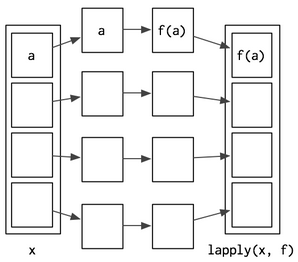
\includegraphics[width=0.30000\textwidth]{Images/10_lapply.PNG}
\caption{\textbf{Abbildung 38}: Wirkungsweise von \emph{lapply()}}
\end{figure}

Aus Gründen der Verarbeitungsgeschwindigkeit ist diese Funktion in C
geschrieben, aber im Wesentlichen entspricht sie folgenden R-Code:

\begin{Shaded}
\begin{Highlighting}[]
\NormalTok{lapply2 <-}\StringTok{ }\ControlFlowTok{function}\NormalTok{(x, f, ...) \{}
\NormalTok{  out <-}\StringTok{ }\KeywordTok{vector}\NormalTok{(}\StringTok{"list"}\NormalTok{, }\KeywordTok{length}\NormalTok{(x))}
  \ControlFlowTok{for}\NormalTok{ (i }\ControlFlowTok{in} \KeywordTok{seq_along}\NormalTok{(x)) \{}
\NormalTok{    out[[i]] <-}\StringTok{ }\KeywordTok{f}\NormalTok{(x[[i]], ...)}
\NormalTok{  \}}
\NormalTok{  out}
\NormalTok{\}}
\end{Highlighting}
\end{Shaded}

Diese Funktion verwendet im Kern einen for-loop. Da innerhalb der
Funktion (\emph{lapply2()}) eine weitere Funktion (\emph{f(x)})
angewendet wird, nennt man das Ganze auch \emph{functional}.

Folgender Code veranschaulicht die Funktionsweise von \emph{lapply}:

\begin{Shaded}
\begin{Highlighting}[]
\CommentTok{# Create some random data}
\NormalTok{  l <-}\StringTok{ }\KeywordTok{replicate}\NormalTok{(}\DecValTok{20}\NormalTok{, }\KeywordTok{runif}\NormalTok{(}\KeywordTok{sample}\NormalTok{(}\DecValTok{1}\OperatorTok{:}\DecValTok{10}\NormalTok{, }\DecValTok{1}\NormalTok{)), }\DataTypeTok{simplify =} \OtherTok{FALSE}\NormalTok{)}
\CommentTok{# With a for loop}
\NormalTok{  out <-}\StringTok{ }\KeywordTok{vector}\NormalTok{(}\StringTok{"list"}\NormalTok{, }\KeywordTok{length}\NormalTok{(l))}
  \ControlFlowTok{for}\NormalTok{ (i }\ControlFlowTok{in} \KeywordTok{seq_along}\NormalTok{(l)) \{}
\NormalTok{    out[[i]] <-}\StringTok{ }\KeywordTok{length}\NormalTok{(l[[i]])}
\NormalTok{  \}}
  \KeywordTok{unlist}\NormalTok{(out)}
\CommentTok{#-------------------------}
\CommentTok{# With lapply}
  \KeywordTok{unlist}\NormalTok{(}\KeywordTok{lapply}\NormalTok{(l, length))}
\CommentTok{#-------------------------  }
\end{Highlighting}
\end{Shaded}

\subsubsection*{\texorpdfstring{\emph{sapply()} und
\emph{vapply()}}{sapply() und vapply()}}\label{sapply-und-vapply}
\addcontentsline{toc}{subsubsection}{\emph{sapply()} und
\emph{vapply()}}

Die beiden funcitonals \emph{sapply()} und \emph{vapply()} funktionieren
im Prinzip gleich wie \emph{lapply()}, mit dem Unterschied, dass der
Output nicht als Liste, sondern als Vektoren zurückgegeben wird.
Betrachte folgenden Anwendung der beiden Funktionen:

\begin{Shaded}
\begin{Highlighting}[]
\KeywordTok{sapply}\NormalTok{(mtcars, is.numeric)}
\KeywordTok{sapply}\NormalTok{(mtcars, mean)}
\KeywordTok{vapply}\NormalTok{(mtcars, is.numeric, }\KeywordTok{logical}\NormalTok{(}\DecValTok{1}\NormalTok{))}
\end{Highlighting}
\end{Shaded}

Beide Funktionen erzielen genau dasselbe Resultat. Die Unterschiede
sind:

\begin{itemize}
\tightlist
\item
  \emph{sapply()} eignet sich besser für interaktives arbeiten, da
  weniger einzugeben ist.
\item
  \emph{vapply()} eignet sich besser bei der Anwendung innerhalb von
  Funktionen, da diese Funktion im Fall von Fehlern während der
  Ausführung weit bessere Rückmeldung an den Programmierer liefert als
  sapply!
\end{itemize}

\subsubsection*{\texorpdfstring{\emph{Map()}}{Map()}}\label{map}
\addcontentsline{toc}{subsubsection}{\emph{Map()}}

Für multiple Inputs eignet sich die \emph{Map()}\footnote{\emph{mapply(\ldots{},
  simpligy = FALSE)} ist die genau dieselbe Funktion wie \emph{Map()}.}
Funkion. Betrachte nachfolgendes Beispiel:

\begin{Shaded}
\begin{Highlighting}[]
  \CommentTok{# Generate some sample data}
\NormalTok{  xs <-}\StringTok{ }\KeywordTok{replicate}\NormalTok{(}\DecValTok{5}\NormalTok{, }\KeywordTok{runif}\NormalTok{(}\DecValTok{10}\NormalTok{), }\DataTypeTok{simplify =} \OtherTok{FALSE}\NormalTok{)}
\NormalTok{  ws <-}\StringTok{ }\KeywordTok{replicate}\NormalTok{(}\DecValTok{5}\NormalTok{, }\KeywordTok{rpois}\NormalTok{(}\DecValTok{10}\NormalTok{, }\DecValTok{5}\NormalTok{) }\OperatorTok{+}\StringTok{ }\DecValTok{1}\NormalTok{, }\DataTypeTok{simplify =} \OtherTok{FALSE}\NormalTok{)}
  \KeywordTok{unlist}\NormalTok{(}\KeywordTok{Map}\NormalTok{(weighted.mean, xs, ws))}
\end{Highlighting}
\end{Shaded}

\subsection*{Die while- und repeat
Schleife}\label{die-while--und-repeat-schleife}
\addcontentsline{toc}{subsection}{Die while- und repeat Schleife}

Ist der Durchlauf von Codezeilen abhängig von einer Bedingung, verwendet
man den while-loop. Betrachte einfach den nachfolgenden Code und
diskutiere die Eigenschaften der Schleife!

\begin{Shaded}
\begin{Highlighting}[]
\NormalTok{  Corr_Resp <-}\StringTok{ }\OtherTok{FALSE}
  \ControlFlowTok{while}\NormalTok{ (Corr_Resp }\OperatorTok{==}\StringTok{ }\OtherTok{FALSE}\NormalTok{) \{}
\NormalTok{    response <-}\StringTok{ }\KeywordTok{readline}\NormalTok{(}\DataTypeTok{prompt =} \StringTok{"What is the correct answer to life, the universe and everything? Please, enter your ANSWER: "}\NormalTok{)}
    \ControlFlowTok{if}\NormalTok{ (response }\OperatorTok{==}\StringTok{ "42"}\NormalTok{) \{}
      \KeywordTok{print}\NormalTok{(}\StringTok{"Cool, you obviously read the right books!"}\NormalTok{)}
\NormalTok{      Corr_Resp <-}\StringTok{ }\OtherTok{TRUE}
\NormalTok{    \} }\ControlFlowTok{else}\NormalTok{ \{}
      \KeywordTok{print}\NormalTok{(}\StringTok{"Sorry, the answer is incorrect, try again!"}\NormalTok{)}
\NormalTok{      \}}
\NormalTok{  \}}
\end{Highlighting}
\end{Shaded}

Wie sofort klar sein sollte, kann es bei while-loops bezüglich der
Abbruchbedingung problematisch werden. Dies gilt auch für den
repeat-loop. Betrachte nachfolgendes Beispiel. Vergleiche dieses mit dem
while-loop und diskutiere den Unterschied!

\begin{Shaded}
\begin{Highlighting}[]
  \ControlFlowTok{repeat}\NormalTok{ \{   }
\NormalTok{    response <-}\StringTok{ }\KeywordTok{readline}\NormalTok{(}\DataTypeTok{prompt =} \StringTok{"What is the correct answer to life, the universe and everything? Please, enter your ANSWER: "}\NormalTok{)}
    \ControlFlowTok{if}\NormalTok{ (response }\OperatorTok{==}\StringTok{ "42"}\NormalTok{) \{}
      \KeywordTok{print}\NormalTok{(}\StringTok{"Cool, you obviously read the right books!"}\NormalTok{);}
      \ControlFlowTok{break}
\NormalTok{    \} }\ControlFlowTok{else} \KeywordTok{print}\NormalTok{(}\StringTok{"Sorry, the answer is incorrect, try again!"}\NormalTok{);}
\NormalTok{  \}}
\end{Highlighting}
\end{Shaded}

\subsubsection*{Aufgabe 2}\label{aufgabe-2-1}
\addcontentsline{toc}{subsubsection}{Aufgabe 2}

Im ersten Schritt soll eine \(m \times n\) Matrix mit lauter Nullen
erstellt werden. Mit einer verschachtelten Schleife soll nun in jede
Zelle die sich unterhalb der Diagonale befindet, das Produkt der
aktuellen Zeile \(\times\) Spalte geschrieben werden. Das Resultat für
eine \(n = 10 \times m = 10\) sollte also folgendermaßen aussehen:

\begin{longtable}[]{@{}cccccccccc@{}}
\toprule
\begin{minipage}[t]{0.05\columnwidth}\centering\strut
0\strut
\end{minipage} & \begin{minipage}[t]{0.05\columnwidth}\centering\strut
0\strut
\end{minipage} & \begin{minipage}[t]{0.05\columnwidth}\centering\strut
0\strut
\end{minipage} & \begin{minipage}[t]{0.05\columnwidth}\centering\strut
0\strut
\end{minipage} & \begin{minipage}[t]{0.05\columnwidth}\centering\strut
0\strut
\end{minipage} & \begin{minipage}[t]{0.05\columnwidth}\centering\strut
0\strut
\end{minipage} & \begin{minipage}[t]{0.05\columnwidth}\centering\strut
0\strut
\end{minipage} & \begin{minipage}[t]{0.05\columnwidth}\centering\strut
0\strut
\end{minipage} & \begin{minipage}[t]{0.05\columnwidth}\centering\strut
0\strut
\end{minipage} & \begin{minipage}[t]{0.05\columnwidth}\centering\strut
0\strut
\end{minipage}\tabularnewline
\begin{minipage}[t]{0.05\columnwidth}\centering\strut
2\strut
\end{minipage} & \begin{minipage}[t]{0.05\columnwidth}\centering\strut
0\strut
\end{minipage} & \begin{minipage}[t]{0.05\columnwidth}\centering\strut
0\strut
\end{minipage} & \begin{minipage}[t]{0.05\columnwidth}\centering\strut
0\strut
\end{minipage} & \begin{minipage}[t]{0.05\columnwidth}\centering\strut
0\strut
\end{minipage} & \begin{minipage}[t]{0.05\columnwidth}\centering\strut
0\strut
\end{minipage} & \begin{minipage}[t]{0.05\columnwidth}\centering\strut
0\strut
\end{minipage} & \begin{minipage}[t]{0.05\columnwidth}\centering\strut
0\strut
\end{minipage} & \begin{minipage}[t]{0.05\columnwidth}\centering\strut
0\strut
\end{minipage} & \begin{minipage}[t]{0.05\columnwidth}\centering\strut
0\strut
\end{minipage}\tabularnewline
\begin{minipage}[t]{0.05\columnwidth}\centering\strut
3\strut
\end{minipage} & \begin{minipage}[t]{0.05\columnwidth}\centering\strut
6\strut
\end{minipage} & \begin{minipage}[t]{0.05\columnwidth}\centering\strut
0\strut
\end{minipage} & \begin{minipage}[t]{0.05\columnwidth}\centering\strut
0\strut
\end{minipage} & \begin{minipage}[t]{0.05\columnwidth}\centering\strut
0\strut
\end{minipage} & \begin{minipage}[t]{0.05\columnwidth}\centering\strut
0\strut
\end{minipage} & \begin{minipage}[t]{0.05\columnwidth}\centering\strut
0\strut
\end{minipage} & \begin{minipage}[t]{0.05\columnwidth}\centering\strut
0\strut
\end{minipage} & \begin{minipage}[t]{0.05\columnwidth}\centering\strut
0\strut
\end{minipage} & \begin{minipage}[t]{0.05\columnwidth}\centering\strut
0\strut
\end{minipage}\tabularnewline
\begin{minipage}[t]{0.05\columnwidth}\centering\strut
4\strut
\end{minipage} & \begin{minipage}[t]{0.05\columnwidth}\centering\strut
8\strut
\end{minipage} & \begin{minipage}[t]{0.05\columnwidth}\centering\strut
12\strut
\end{minipage} & \begin{minipage}[t]{0.05\columnwidth}\centering\strut
0\strut
\end{minipage} & \begin{minipage}[t]{0.05\columnwidth}\centering\strut
0\strut
\end{minipage} & \begin{minipage}[t]{0.05\columnwidth}\centering\strut
0\strut
\end{minipage} & \begin{minipage}[t]{0.05\columnwidth}\centering\strut
0\strut
\end{minipage} & \begin{minipage}[t]{0.05\columnwidth}\centering\strut
0\strut
\end{minipage} & \begin{minipage}[t]{0.05\columnwidth}\centering\strut
0\strut
\end{minipage} & \begin{minipage}[t]{0.05\columnwidth}\centering\strut
0\strut
\end{minipage}\tabularnewline
\begin{minipage}[t]{0.05\columnwidth}\centering\strut
5\strut
\end{minipage} & \begin{minipage}[t]{0.05\columnwidth}\centering\strut
10\strut
\end{minipage} & \begin{minipage}[t]{0.05\columnwidth}\centering\strut
15\strut
\end{minipage} & \begin{minipage}[t]{0.05\columnwidth}\centering\strut
20\strut
\end{minipage} & \begin{minipage}[t]{0.05\columnwidth}\centering\strut
0\strut
\end{minipage} & \begin{minipage}[t]{0.05\columnwidth}\centering\strut
0\strut
\end{minipage} & \begin{minipage}[t]{0.05\columnwidth}\centering\strut
0\strut
\end{minipage} & \begin{minipage}[t]{0.05\columnwidth}\centering\strut
0\strut
\end{minipage} & \begin{minipage}[t]{0.05\columnwidth}\centering\strut
0\strut
\end{minipage} & \begin{minipage}[t]{0.05\columnwidth}\centering\strut
0\strut
\end{minipage}\tabularnewline
\begin{minipage}[t]{0.05\columnwidth}\centering\strut
6\strut
\end{minipage} & \begin{minipage}[t]{0.05\columnwidth}\centering\strut
12\strut
\end{minipage} & \begin{minipage}[t]{0.05\columnwidth}\centering\strut
18\strut
\end{minipage} & \begin{minipage}[t]{0.05\columnwidth}\centering\strut
24\strut
\end{minipage} & \begin{minipage}[t]{0.05\columnwidth}\centering\strut
30\strut
\end{minipage} & \begin{minipage}[t]{0.05\columnwidth}\centering\strut
0\strut
\end{minipage} & \begin{minipage}[t]{0.05\columnwidth}\centering\strut
0\strut
\end{minipage} & \begin{minipage}[t]{0.05\columnwidth}\centering\strut
0\strut
\end{minipage} & \begin{minipage}[t]{0.05\columnwidth}\centering\strut
0\strut
\end{minipage} & \begin{minipage}[t]{0.05\columnwidth}\centering\strut
0\strut
\end{minipage}\tabularnewline
\begin{minipage}[t]{0.05\columnwidth}\centering\strut
7\strut
\end{minipage} & \begin{minipage}[t]{0.05\columnwidth}\centering\strut
14\strut
\end{minipage} & \begin{minipage}[t]{0.05\columnwidth}\centering\strut
21\strut
\end{minipage} & \begin{minipage}[t]{0.05\columnwidth}\centering\strut
28\strut
\end{minipage} & \begin{minipage}[t]{0.05\columnwidth}\centering\strut
35\strut
\end{minipage} & \begin{minipage}[t]{0.05\columnwidth}\centering\strut
42\strut
\end{minipage} & \begin{minipage}[t]{0.05\columnwidth}\centering\strut
0\strut
\end{minipage} & \begin{minipage}[t]{0.05\columnwidth}\centering\strut
0\strut
\end{minipage} & \begin{minipage}[t]{0.05\columnwidth}\centering\strut
0\strut
\end{minipage} & \begin{minipage}[t]{0.05\columnwidth}\centering\strut
0\strut
\end{minipage}\tabularnewline
\begin{minipage}[t]{0.05\columnwidth}\centering\strut
8\strut
\end{minipage} & \begin{minipage}[t]{0.05\columnwidth}\centering\strut
16\strut
\end{minipage} & \begin{minipage}[t]{0.05\columnwidth}\centering\strut
24\strut
\end{minipage} & \begin{minipage}[t]{0.05\columnwidth}\centering\strut
32\strut
\end{minipage} & \begin{minipage}[t]{0.05\columnwidth}\centering\strut
40\strut
\end{minipage} & \begin{minipage}[t]{0.05\columnwidth}\centering\strut
48\strut
\end{minipage} & \begin{minipage}[t]{0.05\columnwidth}\centering\strut
56\strut
\end{minipage} & \begin{minipage}[t]{0.05\columnwidth}\centering\strut
0\strut
\end{minipage} & \begin{minipage}[t]{0.05\columnwidth}\centering\strut
0\strut
\end{minipage} & \begin{minipage}[t]{0.05\columnwidth}\centering\strut
0\strut
\end{minipage}\tabularnewline
\begin{minipage}[t]{0.05\columnwidth}\centering\strut
9\strut
\end{minipage} & \begin{minipage}[t]{0.05\columnwidth}\centering\strut
18\strut
\end{minipage} & \begin{minipage}[t]{0.05\columnwidth}\centering\strut
27\strut
\end{minipage} & \begin{minipage}[t]{0.05\columnwidth}\centering\strut
36\strut
\end{minipage} & \begin{minipage}[t]{0.05\columnwidth}\centering\strut
45\strut
\end{minipage} & \begin{minipage}[t]{0.05\columnwidth}\centering\strut
54\strut
\end{minipage} & \begin{minipage}[t]{0.05\columnwidth}\centering\strut
63\strut
\end{minipage} & \begin{minipage}[t]{0.05\columnwidth}\centering\strut
72\strut
\end{minipage} & \begin{minipage}[t]{0.05\columnwidth}\centering\strut
0\strut
\end{minipage} & \begin{minipage}[t]{0.05\columnwidth}\centering\strut
0\strut
\end{minipage}\tabularnewline
\begin{minipage}[t]{0.05\columnwidth}\centering\strut
10\strut
\end{minipage} & \begin{minipage}[t]{0.05\columnwidth}\centering\strut
20\strut
\end{minipage} & \begin{minipage}[t]{0.05\columnwidth}\centering\strut
30\strut
\end{minipage} & \begin{minipage}[t]{0.05\columnwidth}\centering\strut
40\strut
\end{minipage} & \begin{minipage}[t]{0.05\columnwidth}\centering\strut
50\strut
\end{minipage} & \begin{minipage}[t]{0.05\columnwidth}\centering\strut
60\strut
\end{minipage} & \begin{minipage}[t]{0.05\columnwidth}\centering\strut
70\strut
\end{minipage} & \begin{minipage}[t]{0.05\columnwidth}\centering\strut
80\strut
\end{minipage} & \begin{minipage}[t]{0.05\columnwidth}\centering\strut
90\strut
\end{minipage} & \begin{minipage}[t]{0.05\columnwidth}\centering\strut
0\strut
\end{minipage}\tabularnewline
\bottomrule
\end{longtable}

Verwende den nachstehenden Code um die Aufgabe zu lösen. Ersetze dabei
die Platzhalter (\emph{XXX}) durch die entsprechenden Indices,
Variablen, etc.

\begin{Shaded}
\begin{Highlighting}[]
  \CommentTok{# Make a lower triangular matrix (zeroes in upper right corner)}
\NormalTok{  m     <-}\StringTok{ }\DecValTok{10} \CommentTok{# number of rows in matrix}
\NormalTok{  n     <-}\StringTok{ }\DecValTok{10} \CommentTok{# number of columnes in matrix}
\NormalTok{  ctr   <-}\StringTok{ }\DecValTok{0}  \CommentTok{# a counter to count the assignment}
\NormalTok{  mymat <-}\StringTok{ }\KeywordTok{matrix}\NormalTok{(}\DataTypeTok{data =} \DecValTok{0}\NormalTok{, }\DataTypeTok{nrow =}\NormalTok{ m, }\DataTypeTok{ncol =}\NormalTok{ n) }\CommentTok{# Create a 10 x 10 matrix with zeroes }
  \ControlFlowTok{for}\NormalTok{(i }\ControlFlowTok{in} \DecValTok{1} \OperatorTok{:}\StringTok{ }\NormalTok{XXX) \{}
    \ControlFlowTok{for}\NormalTok{(j }\ControlFlowTok{in} \DecValTok{1} \OperatorTok{:}\StringTok{ }\NormalTok{XXX) \{   }
      \ControlFlowTok{if}\NormalTok{(XXX }\OperatorTok{==}\StringTok{ }\NormalTok{XXX) \{ }
        \ControlFlowTok{break}\NormalTok{;}
\NormalTok{      \} }\ControlFlowTok{else}\NormalTok{ \{}
        \CommentTok{# you assign the values only when i<>j}
\NormalTok{        mymat[XXX,XXX] <-}\StringTok{ }\NormalTok{XXX }\OperatorTok{*}\StringTok{ }\NormalTok{XXX}
\NormalTok{        ctr        <-}\StringTok{ }\NormalTok{ctr }\OperatorTok{+}\StringTok{ }\DecValTok{1}
\NormalTok{      \}}
\NormalTok{    \}}
    \KeywordTok{print}\NormalTok{(XXX }\OperatorTok{*}\StringTok{ }\NormalTok{XXX) }
\NormalTok{  \}}
  \KeywordTok{print}\NormalTok{(}\KeywordTok{paste}\NormalTok{(}\StringTok{'There are'}\NormalTok{, XXX, }\StringTok{"cells in the matrix"}\NormalTok{))  }\CommentTok{# Print how many matrix cells were assigned}
  \KeywordTok{print}\NormalTok{(}\KeywordTok{paste}\NormalTok{(}\StringTok{'There are'}\NormalTok{, XXX, }\StringTok{"cells assigned with values in the matrix"}\NormalTok{))  }\CommentTok{# Print how many matrix cells were assigned  }
\end{Highlighting}
\end{Shaded}

\protect\hyperlink{aufgabe-2-lsg}{Hier findest du die Lösung zur
Aufgabe}.

\subsection*{Lösungen}\label{losungen-4}
\addcontentsline{toc}{subsection}{Lösungen}

\hypertarget{aufgabe-1-lsg}{\subsubsection*{Aufgabe 1
Lsg}\label{aufgabe-1-lsg}}
\addcontentsline{toc}{subsubsection}{Aufgabe 1 Lsg}

\begin{Shaded}
\begin{Highlighting}[]
\NormalTok{  punkte <-}\StringTok{ }\DecValTok{85}
  \ControlFlowTok{if}\NormalTok{ (punkte }\OperatorTok{>=}\StringTok{ }\DecValTok{90}\NormalTok{) \{}
    \KeywordTok{print}\NormalTok{(}\StringTok{"Sehr gut"}\NormalTok{)}
\NormalTok{  \} }\ControlFlowTok{else} \ControlFlowTok{if}\NormalTok{ (punkte }\OperatorTok{>=}\StringTok{ }\DecValTok{80} \OperatorTok{&}\StringTok{ }\NormalTok{punkte }\OperatorTok{<}\StringTok{ }\DecValTok{90}\NormalTok{) \{}
    \KeywordTok{print}\NormalTok{(}\StringTok{"Gut"}\NormalTok{);    }
\NormalTok{  \} }\ControlFlowTok{else} \ControlFlowTok{if}\NormalTok{ (punkte }\OperatorTok{>=}\StringTok{ }\DecValTok{70} \OperatorTok{&}\StringTok{ }\NormalTok{punkte }\OperatorTok{<}\StringTok{ }\DecValTok{90}\NormalTok{) \{}
    \KeywordTok{print}\NormalTok{(}\StringTok{"Befriedigend"}\NormalTok{);    }
\NormalTok{  \} }\ControlFlowTok{else} \ControlFlowTok{if}\NormalTok{ (punkte }\OperatorTok{>=}\StringTok{ }\DecValTok{60} \OperatorTok{&}\StringTok{ }\NormalTok{punkte }\OperatorTok{<}\StringTok{ }\DecValTok{70}\NormalTok{) \{}
    \KeywordTok{print}\NormalTok{(}\StringTok{"genügend"}\NormalTok{);    }
\NormalTok{  \} }\ControlFlowTok{else}\NormalTok{ \{}
    \KeywordTok{print}\NormalTok{(}\StringTok{"Nicht genügend"}\NormalTok{);    }
\NormalTok{  \}}
\end{Highlighting}
\end{Shaded}

\protect\hyperlink{aufgabe-1}{zurück zur Aufgabe}

\hypertarget{aufgabe-2-lsg}{\subsubsection*{Aufgabe 2
Lsg}\label{aufgabe-2-lsg}}
\addcontentsline{toc}{subsubsection}{Aufgabe 2 Lsg}

\begin{Shaded}
\begin{Highlighting}[]
  \CommentTok{# Make a lower triangular matrix (zeroes in upper right corner)}
\NormalTok{  m     <-}\StringTok{ }\DecValTok{10} \CommentTok{# number of rows in matrix}
\NormalTok{  n     <-}\StringTok{ }\DecValTok{10} \CommentTok{# number of columnes in matrix}
\NormalTok{  ctr   <-}\StringTok{ }\DecValTok{0}  \CommentTok{# a counter to count the assignment}
\NormalTok{  mymat <-}\StringTok{ }\KeywordTok{matrix}\NormalTok{(}\DataTypeTok{data =} \DecValTok{0}\NormalTok{, }\DataTypeTok{nrow =}\NormalTok{ m, }\DataTypeTok{ncol =}\NormalTok{ n) }\CommentTok{# Create a 10 x 10 matrix with zeroes }
  \ControlFlowTok{for}\NormalTok{(i }\ControlFlowTok{in} \DecValTok{1} \OperatorTok{:}\StringTok{ }\NormalTok{m) \{}
    \ControlFlowTok{for}\NormalTok{(j }\ControlFlowTok{in} \DecValTok{1} \OperatorTok{:}\StringTok{ }\NormalTok{n) \{   }
      \ControlFlowTok{if}\NormalTok{(i }\OperatorTok{==}\StringTok{ }\NormalTok{j) \{ }
        \ControlFlowTok{break}\NormalTok{;}
\NormalTok{      \} }\ControlFlowTok{else}\NormalTok{ \{}
        \CommentTok{# you assign the values only when i<>j}
\NormalTok{        mymat[i,j] <-}\StringTok{ }\NormalTok{i }\OperatorTok{*}\StringTok{ }\NormalTok{j}
\NormalTok{        ctr        <-}\StringTok{ }\NormalTok{ctr }\OperatorTok{+}\StringTok{ }\DecValTok{1}
\NormalTok{      \}}
\NormalTok{    \}}
    \KeywordTok{print}\NormalTok{(i }\OperatorTok{*}\StringTok{ }\NormalTok{j) }
\NormalTok{  \}}
  \KeywordTok{print}\NormalTok{(}\KeywordTok{paste}\NormalTok{(}\StringTok{'There are'}\NormalTok{, }\KeywordTok{length}\NormalTok{(mymat), }\StringTok{"cells in the matrix"}\NormalTok{))  }\CommentTok{# Print how many matrix cells were assigned}
  \KeywordTok{print}\NormalTok{(}\KeywordTok{paste}\NormalTok{(}\StringTok{'There are'}\NormalTok{, ctr, }\StringTok{"cells assigned with values in the matrix"}\NormalTok{))  }\CommentTok{# Print how many matrix cells were assigned}
\end{Highlighting}
\end{Shaded}

\protect\hyperlink{aufgabe-2}{zurück zur Aufgabe}


\end{document}
